\chapter{Semi-classical Wavepackets}
\label{ch:wavepackets}


\section{The basis functions}


We first show once more the one-dimensional semi-classical wavepackets.
This short section will constitute a reference to compare with when
we will head for the $D$-dimensional case. The full mathematical details
can be found in \cite{H_ladder_operators}.


\subsection{The one-dimensional case}


In the 1-dimensional case the semi-classical Hagedorn wavepacket is defined as:

\begin{align} \label{eq:phi0_1d}
  \phi_0[\Pi](x) & = \pi^{-\frac{1}{4}} (\varepsilon^2)^{-\frac{1}{4}} Q^{-\frac{1}{2}}
                     \exp \left( i PQ\inv (x-q)^2 / (2\varepsilon^2) + i p (x-q) / \varepsilon^2 \right) \\
                 & \assign (\pi\varepsilon^2)^{-\frac{1}{4}} Q^{-\frac{1}{2}}
                           \exp \left( \frac{i}{2\varepsilon^2} PQ\inv (x-q)^2 + \frac{i}{\varepsilon^2} p (x-q) \right)
\end{align}

where $x, q, p \in \mathbb{R}$ and $Q, P \in \mathbb{C}$ some parameters. We gather
them into the set $\Pi \assign {q,p,Q,P}$ which we often call the \emph{Hagedorn parameter}.
For these parameters, there is a condition that must hold:

\begin{align} \label{eq:PQcond_1d}
  \conj{Q} P - \conj{P} Q & = 2i \\
  P Q - Q P & = 0 \,.
\end{align}

The second equation is trivial in the one-dimensional case because complex numbers
commute.

The equation \eqref{eq:phi0_1d} represents some kind of ground state $\phi_0$. We
can construct higher order states $\phi_k$ by the help of raising operators. The
raising operator $\mathcal{R}$ and lowering operator $\mathcal{L}$ are defined
as:

\begin{align} \label{eq:raising_ops_1d}
  \mathcal{R} & =  \frac{i}{\sqrt{2\varepsilon^2}} \left( \conj{P} (x-q) - \conj{Q} (y-p) \right) \\
  \mathcal{L} & = -\frac{i}{\sqrt{2\varepsilon^2}} \left( P (x-q) - Q (y-p) \right)
\end{align}

where $y$ denotes the momentum operator $y \assign -i\varepsilon^2 \pdiff{}{x}$.
See \cite{B_bachelor_thesis} for the details of the one-dimensional case.
Applied to the function $\phi_0$ we get:

\begin{equation}
  \phi_k = \frac{1}{\sqrt{k}} \mathcal{R}^k \phi_0
\end{equation}

by repeated application of $\mathcal{R}$. For a single application to the function
$\phi_k$ we know that:

\begin{align}
  \phi_{k-1} = \frac{1}{\sqrt{k}} \mathcal{L} \phi_k \\
  \phi_{k+1} = \frac{1}{\sqrt{k+1}} \mathcal{R} \phi_k \,.
\end{align}

In principle we can now write the expression for $\phi_k$ in closed-form:

\begin{align*}
  \phi_k[\Pi](x) = \, & 2^{-\frac{k}{2}} (k!)^{-\frac{1}{2}} (\pi\varepsilon^2)^{-\frac{1}{4}}
                     Q^{-\frac{k+1}{2}} \conj{Q}^{\frac{k}{2}}
                     H_k \left(\varepsilon^{-1} |Q|^{-1} (x-q) \right) \cdot \\
                   & \exp \left( \frac{i}{2\varepsilon^2} PQ\inv (x-q)^2 + \frac{i}{\varepsilon^2} p (x-q) \right)
\end{align*}

where the Hermite polynomials $H_k$ are defined as $H_k(z) \assign e^{z^2} \left(-\pdiff{}{z} \right)^k e^{-z^2}$.
Although we have this closed-form expression for $\phi_k$ we will never use it
due to numerical issues for example with the factorial there.

With the use of the ladder operators we can find a three-term recursion formula
involving $\phi_{k+1}$ , $\phi_k$ and $\phi_{k-1}$ only:

\begin{equation}
  \phi_{k+1}(x) = \sqrt{\frac{2}{\varepsilon^2}} \frac{1}{\sqrt{k+1}} Q^{-1} (x-q) \phi_k(x)
                  -\sqrt{\frac{k}{k+1}} Q^{-1} \conj{Q} \phi_{k-1}(x) \,.
\end{equation}

For this recursive computation we need two starting points. Obviously we use
$\phi_0$ which we can compute easily. For the second point we could use
$\phi_1 = \mathcal{R} \phi_0 = \sqrt{\frac{2}{\varepsilon^2}} Q^{-1} (x-q) \phi_0(x)$
which we can find by hand. Alternatively we can use the fundamental property of
the lowering operator $\mathcal{L} \phi_0 \equiv 0$ and find that $\phi_{-1} \equiv 0$.
Although this appears to be a very technical argument it works fine.


\subsection{The multi-dimensional case}


In the $D$-dimensional case everything works analogously but also becomes more
complicated. However we can check correctness of the results by taking $D=1$.
All formulae from the last section have to be contained as special cases.

First we note that $\vec{x} \in \mathbb{R}^D$ is a vector with $D$ components
denoted by $\vec{x} = (x_0, \ldots, x_{D-1})$. It follows that the position and momentum
means are also vectors, in short $\vec{q}, \vec{p} \in \mathbb{R}^D$. The parameters
$\mat{Q}, \mat{P} \in \mathbb{C}^{D \times D}$ are hence complex matrices of shape
$D \times D$. For these matrices two relations analogue to \eqref{eq:PQcond_1d}
hold:

\begin{align} \label{eq:PQcond_Dd}
  \mat{Q}\H \mat{P} - \mat{P}\H \mat{Q} & = 2i \id \\
  \mat{P}\T \mat{Q} - \mat{Q}\T \mat{P} & = \mat{0} \,.
\end{align}

The ground state $\phi_{\vec{0}}$ can now be defined as:

\begin{align}  \label{eq:phi0_Dd}
  \phi_{\vec{0}}[\Pi]\left(\vec{x}\right)
  \assign
  (\pi\varepsilon^2)^{-\frac{D}{4}} (\det\mat{Q})^{-\frac{1}{2}}
  \exp \left( \frac{i}{2\varepsilon^2}
  \dotp{(\vec{x}-\vec{q})}{\mat{P}\mat{Q}\inv(\vec{x}-\vec{q})}
  + \frac{i}{\varepsilon^2} \dotp{\vec{p}}{(\vec{x}-\vec{q})}
 \right) \,.
\end{align}

We will see soon that we have to index it by a multi-index $\vec{0} \assign (0, \ldots, 0)$
instead of a simple $0$.


\section{Raising and lowering operators}


Defining the raising and lowering operators is not as trivial as in the
one-dimensional case. We have no linear arrangement of all functions $\phi_{\vec{k}}$.
In fact the index $\vec{k}$ is a vector- or multi-index:

\begin{equation}
  \vec{k} \assign ( k_0, \ldots, k_{D-1} ) \in \mathbb{N}_0^D \,.
\end{equation}

Its \emph{length} is defined as:

\begin{equation}
  |\vec{k}| \assign \sum_{i=0}^{D-1} k_i
\end{equation}

and its \emph{factorial} as:

\begin{equation}
  \vec{k}! \assign (k_0!)(k_1!)\cdots(k_{D-1}!) = \prod_{i=0}^{D-1} k_i! \,.
\end{equation}

In the following we will set $D=2$ for most examples. In the two-dimensional case
we take $\vec{k} = (k,l)$ and get the grid of functions $\phi_{k,l}$ indexed by
two non-negative integers $k$ and $l$ as shown in figure \ref{fig:phi_kl_grid}.

\begin{figure}
  \centering
  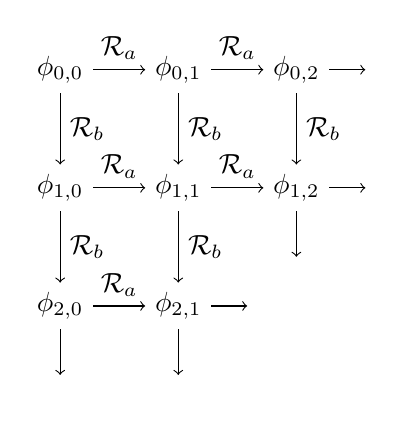
\begin{tikzpicture}[node distance=1.5cm, auto]
  \node (phi00) {$\phi_{0,0}$};
  \node (phi01) [right of=phi00] {$\phi_{0,1}$};
  \node (phi02) [right of=phi01] {$\phi_{0,2}$};
  \node (phi03) [right of=phi02, node distance=1cm] {$ $};

  \node (phi10) [below of=phi00] {$\phi_{1,0}$};
  \node (phi11) [right of=phi10] {$\phi_{1,1}$};
  \node (phi12) [right of=phi11] {$\phi_{1,2}$};
  \node (phi13) [right of=phi12, node distance=1cm] {$ $};

  \node (phi20) [below of=phi10] {$\phi_{2,0}$};
  \node (phi21) [right of=phi20] {$\phi_{2,1}$};
  \node (phi22a) [right of=phi21, node distance=1cm] {$ $};
  \node (phi22b) [below of=phi12, node distance=1cm] {$ $};

  \node (phi30) [below of=phi20, node distance=1cm] {$ $};
  \node (phi31) [below of=phi21, node distance=1cm] {$ $};

  \draw[->] (phi00) to node {$\mathcal{R}_a$} (phi01);
  \draw[->] (phi01) to node {$\mathcal{R}_a$} (phi02);
  \draw[->] (phi02) to node {$ $} (phi03);

  \draw[->] (phi10) to node {$\mathcal{R}_a$} (phi11);
  \draw[->] (phi11) to node {$\mathcal{R}_a$} (phi12);
  \draw[->] (phi12) to node {$ $} (phi13);

  \draw[->] (phi20) to node {$\mathcal{R}_a$} (phi21);
  \draw[->] (phi21) to node {$ $} (phi22a);

  \draw[->] (phi00) to node {$\mathcal{R}_b$} (phi10);
  \draw[->] (phi10) to node {$\mathcal{R}_b$} (phi20);
  \draw[->] (phi20) to node {$ $} (phi30);

  \draw[->] (phi01) to node {$\mathcal{R}_b$} (phi11);
  \draw[->] (phi11) to node {$\mathcal{R}_b$} (phi21);
  \draw[->] (phi21) to node {$ $} (phi31);

  \draw[->] (phi02) to node {$\mathcal{R}_b$} (phi12);
  \draw[->] (phi12) to node {$ $} (phi22b);
\end{tikzpicture}

  \caption{The grid of basis functions $\phi_{k,l}$ for the case $D=2$.}
  \label{fig:phi_kl_grid}
\end{figure}

Every arrow stands for a raising operator $\mathcal{R}$ and we see that there are
two kinds of arrows, vertical and horizontal ones. Following an arrow only one
of the two indices $(k,l)$ changes. This is shown in more details in figure
\ref{fig:phi_kl_operators}.

\begin{figure}[h!]
  \centering
  \subfloat[][]{
    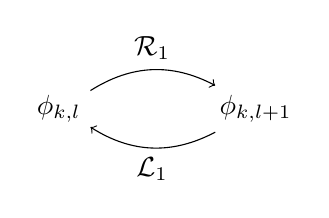
\begin{tikzpicture}[node distance=2.5cm, auto]
  \node (phikl) {$\phi_{k,l}$};
  \node (phikll) [right of=phikl] {$\phi_{k,l+1}$};
  \draw[->] (phikl) to [bend left] node {$\mathcal{R}_1$} (phikll);
  \draw[->] (phikll) to [bend left] node {$\mathcal{L}_1$} (phikl);
\end{tikzpicture}

  }
  \subfloat[][]{
    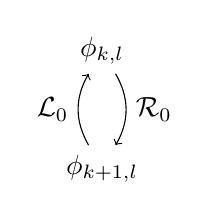
\begin{tikzpicture}[node distance=1.5cm, auto]
  \node (phikl) {$\phi_{k,l}$};
  \node (phikkl) [below of=phikl] {$\phi_{k+1,l}$};
  \draw[->] (phikl) to [bend left] node {$\mathcal{R}_0$} (phikkl);
  \draw[->] (phikkl) to [bend left] node {$\mathcal{L}_0$} (phikl);
\end{tikzpicture}

  } \\
    \caption[]{The two raising and lowering operator pairs in action.}
    \label{fig:phi_kl_operators}
\end{figure}

This fact suggests that we assign a raising operator to each arrow type hence we
get two operators $\mathcal{R}_0$ and $\mathcal{R}_1$ which are of different
nature. We can assign a distinct set $\{\mathcal{R}_i, \mathcal{L}_i\}$ to each
axis $i \in [0, \ldots, D-1]$ of the lattice.

Leaving this introductionary example and following the formal derivation from
\cite{H_ladder_operators} now, we take $\vec{v} \in \mathbb{C}^D$, define
$\vec{y} \assign -i \varepsilon^2 \nabla_x$ and begin with:

\begin{align}
  \mathcal{R}_v & \assign \frac{1}{\sqrt{2\varepsilon^2}}
                  \left(
                    \dotp{-i\mat{P}\vec{\conj{v}}}{(\vec{x}-\vec{q})}
                    -i \dotp{\mat{Q}\vec{\conj{v}}}{(\vec{y}-\vec{p})}
                  \right) \\
                & = \frac{1}{\sqrt{2\varepsilon^2}}
                  \left(
                    i \dotp{\mat{P}\vec{\conj{v}}}{(\vec{x}-\vec{q})}
                    -i \dotp{\mat{Q}\vec{\conj{v}}}{(\vec{y}-\vec{p})}
                  \right) \\
                & = \frac{i}{\sqrt{2\varepsilon^2}}
                  \left(
                    \dotp{\mat{P}\vec{\conj{v}}}{(\vec{x}-\vec{q})}
                    - \dotp{\mat{Q}\vec{\conj{v}}}{(\vec{y}-\vec{p})}
                  \right)
\end{align}

and similarly we get:

\begin{align}
  \mathcal{L}_v & \assign \frac{1}{\sqrt{2\varepsilon^2}}
                  \left(
                    \dotp{\conj{-i \mat{P}}\vec{v}}{(\vec{x}-\vec{q})}
                    +i \dotp{\mat{\conj{Q}}\vec{v}}{(\vec{y}-\vec{p})}
                  \right) \\
                & = \frac{1}{\sqrt{2\varepsilon^2}}
                  \left(
                    -i \dotp{\mat{\conj{P}}\vec{v}}{(\vec{x}-\vec{q})}
                    +i \dotp{\mat{\conj{Q}}\vec{v}}{(\vec{y}-\vec{p})}
                  \right) \\
                & = -\frac{i}{\sqrt{2\varepsilon^2}}
                  \left(
                    \dotp{\mat{\conj{P}}\vec{v}}{(\vec{x}-\vec{q})}
                    - \dotp{\mat{\conj{Q}}\vec{v}}{(\vec{y}-\vec{p})}
                  \right) \,.
\end{align}

For the one-dimensional case we can get back at the definitions from \eqref{eq:raising_ops_1d}.
Following along the lines of \cite{H_ladder_operators} we can compute several commutators:

\begin{align}
  [\mathcal{L}_v, \mathcal{L}_w] & = \mathcal{L}_v\mathcal{L}_w - \mathcal{L}_w\mathcal{L}_v = 0 \\
  [\mathcal{R}_v, \mathcal{R}_w] & = \mathcal{R}_v\mathcal{R}_w - \mathcal{R}_w\mathcal{R}_v = 0 \\
  [\mathcal{L}_v, \mathcal{R}_w] & = \mathcal{L}_v\mathcal{R}_w - \mathcal{R}_w\mathcal{L}_v = \dotp{\vec{v}}{\vec{w}}
\end{align}

for general $\vec{v}, \vec{w} \in \mathbb{C}^D$. The fact that we are allowed to
interchange two raising operators is important and could have been guessed from
figure \ref{fig:phi_kl_grid}. There we have:

\begin{align*}
  \phi_{1,1} & = \mathcal{R}_0 \phi_{0,1} = \mathcal{R}_0 \mathcal{R}_1 \phi_{0,0} \\
  \phi_{1,1} & = \mathcal{R}_1 \phi_{1,0} = \mathcal{R}_1 \mathcal{R}_0 \phi_{0,0}
\end{align*}

thus the order in which we compute $\phi_{k,l}$ from $\phi_{0,0}$ does not matter.
If we flip all arrows we get to the same conclusion but this time for lowering
operators.

From the scalar case we know that we can not simply exchange two different
operators, remember for example the definition of the number operator $\mathcal{N}$.
However, we can go from $\phi_{1,0}$ to $\phi_{0,1}$ by either way:

\begin{align*}
  \phi_{0,1} & = \mathcal{L}_0 \phi_{1,1} = \mathcal{L}_0 \mathcal{R}_1 \phi_{1,0} \\
  \phi_{0,1} & = \mathcal{R}_1 \phi_{0,0} = \mathcal{R}_1 \mathcal{L}_0 \phi_{1,0} \,.
\end{align*}

This is the consequence of the third commutation relation above which tells us
that the two operators commute iff $\vec{v}$ and $\vec{w}$ are orthogonal.

Continuing with the formal derivation we choose a basis of $\mathbb{R}^D$. For
simplicity we take the canonical basis $\{\vec{e}^j\}_{j=0}^{D-1}$. In this basis
we can more precisely say what $\mathcal{R}_v$ is. We define the following two
sets of ladder operators:

\begin{align}
  \mathcal{R}_j & \assign \mathcal{R}_{e^j} \\
  \mathcal{L}_j & \assign \mathcal{L}_{e^j}
\end{align}

each containing exactly $D$ operators. Finally we can build the vector-valued
operators:

\begin{equation} \label{eq:raising_ops_Dd_vectorial}
  \mathcal{R} \assign
  \begin{pmatrix}
    \mathcal{R}_0 \\
    \vdots \\
    \mathcal{R}_{D-1}
  \end{pmatrix}
  \qquad \text{and} \qquad
  \mathcal{L} \assign
  \begin{pmatrix}
    \mathcal{L}_0 \\
    \vdots \\
    \mathcal{L}_{D-1}
  \end{pmatrix} \,.
\end{equation}

Recalling the defining equations for $\mathcal{R}_v$ and $\mathcal{L}_v$ we can
then find explicit expressions for $\mathcal{R}$ and $\mathcal{L}$:

\begin{align} \label{eq:raising_ops_Dd_explicit}
  \mathcal{R} & =  \frac{i}{\sqrt{2\varepsilon^2}} \left( \mat{P}\H (\vec{x}-\vec{q}) - \mat{Q}\H (\vec{y}-\vec{p}) \right) \\
  \mathcal{L} & = -\frac{i}{\sqrt{2\varepsilon^2}} \left( \mat{P}\T (\vec{x}-\vec{q}) - \mat{Q}\T (\vec{y}-\vec{p}) \right) \,.
\end{align}

At this point we should stop for a moment and see what happens if we set $D=1$ now.
If we carried out all calculations we would return step by step to the expressions
given in \eqref{eq:raising_ops_1d}.

With the help of $\mathcal{R}$ we can now go on and define all higher states
$\phi_{\vec{k}}$ properly:

\begin{align} \label{eq:construct_phi_k}
  \phi_{\vec{k}} & \assign \mathcal{R}^{\vec{k}} \phi_{\vec{0}} \\
                 & = \frac{1}{\sqrt{\vec{k}!}} \mathcal{R}_0^{k_0} \mathcal{R}_1^{k_1} \cdots \mathcal{R}_{D-1}^{k_{D-1}} \phi_{\vec{0}} \\
                 & = \frac{1}{\sqrt{\prod_{i=0}^{D-1}k_i!}} \prod_{i=0}^{D-1} \mathcal{R}_i^{k_i} \phi_{\vec{0}} \,.
\end{align}

We can show theorem 3.3 of \cite{H_ladder_operators}:

\begin{theorem}
  The functions $\phi_{\vec{k}}\left[\Pi\right](\vec{x})$ form an orthonormal
  basis of $L^2 \left(\mathbb{R}^D \right)$.
\end{theorem}

For a proof see again this reference.

To close this section we take a closer look at the application of $\mathcal{R}_j$
on $\phi_{\vec{k}}$:

\begin{equation} \label{eq:r_op_applied_1}
  \mathcal{R}_j \phi_{\vec{k}} = \sqrt{k_j + 1} \phi_{\vec{k}^\prime}
\end{equation}

where:

\begin{equation}
  \vec{k}^\prime \assign \vec{k} + \vec{e}^j = (k_0, \ldots, k_{j-1}, k_j+1, k_{j+1}, \ldots, k_{D-1})
\end{equation}

and similarly:

\begin{equation}
  \mathcal{L}_j \phi_{\vec{k}} = \sqrt{k_j} \phi_{\vec{k}^\prime}
\end{equation}

with:

\begin{equation}
  \vec{k}^\prime \assign \vec{k} - \vec{e}^j = (k_0, \ldots, k_{j-1}, k_j-1, k_{j+1}, \ldots, k_{D-1}) \,.
\end{equation}

This justifies the formula \eqref{eq:construct_phi_k} allowing us to construct
$\phi_{\vec{k}}$ out of $\phi_{\vec{0}}$ by raising each index multiple times as
necessary. We build a path through the lattice starting at the origin and ending
at the point $\vec{k}$.

From these formula we see that computing $\mathcal{R} \phi_{\vec{0}}$ is sufficient
to access all higher order functions. The remaining question is how to do this
efficiently. Computing the action of $\mathcal{R}$ is not straight forward because
it contains the differential operator $y \assign -i \varepsilon^2 \nabla_x$. For
this reason we seek a way to compute $\mathcal{R} \phi_{\vec{0}}$ without
ever applying $y$ explicitly. The solution to this task is given by the adjoint
pair $\mathcal{R}, \mathcal{L}$ of operators. We can set up a system of two
operator equations. First we solve the equation defining $\mathcal{L}$ for $y$.
For simplicity of notation we define $\theta \assign \frac{i}{\sqrt{2\varepsilon^2}}$
and transform as follows:

\begin{align} \label{eq:y_op}
  \mathcal{L} & = -\theta \left( \mat{P}\T (\vec{x}-\vec{q}) - \mat{Q}\T (\vec{y}-\vec{p}) \right) \nonumber\\
  \mathcal{L} & = -\theta \mat{P}\T (\vec{x}-\vec{q}) + \theta \mat{Q}\T (\vec{y}-\vec{p}) \nonumber\\
  \mathcal{L} + \theta \mat{P}\T (\vec{x}-\vec{q}) & = \theta \mat{Q}\T (\vec{y}-\vec{p}) \nonumber\\
  \mat{Q}\T (\vec{y}-\vec{p}) & = \frac{1}{\theta} \mathcal{L} + \mat{P}\T (\vec{x}-\vec{q}) \nonumber\\
  \vec{y}-\vec{p} & = \frac{1}{\theta} \mat{Q}\Tinv \mathcal{L} + \mat{Q}\Tinv \mat{P}\T (\vec{x}-\vec{q}) \nonumber\\
  \vec{y} & = \frac{1}{\theta} \mat{Q}\Tinv \mathcal{L} + \mat{Q}\Tinv \mat{P}\T (\vec{x}-\vec{q}) + \vec{p} \,.
\end{align}

Note that solving $\mathcal{R}$ for $y$ gives us the complex conjugate of this
last line:

\begin{equation}  \label{eq:y_op_cc}
  \vec{y} = -\frac{1}{\theta} \mat{Q}\Hinv \mathcal{R} + \mat{Q}\Hinv \mat{P}\H (\vec{x}-\vec{q}) + \vec{p} \,.
\end{equation}

In the next step we plug the result \eqref{eq:y_op} into the definition of
$\mathcal{R}$:

\begin{align} \label{eq:loc_op_r}
  \mathcal{R} & = \theta \left( \mat{P}\H (\vec{x}-\vec{q}) - \mat{Q}\H (\vec{y}-\vec{p}) \right) \nonumber\\
  \mathcal{R} & = \theta \left( \mat{P}\H (\vec{x}-\vec{q}) - \mat{Q}\H \left(\left(
                  \frac{1}{\theta} \mat{Q}\Tinv \mathcal{L} + \mat{Q}\Tinv \mat{P}\T (\vec{x}-\vec{q}) + \vec{p}
                  \right)-\vec{p}\right) \right) \nonumber\\
  \mathcal{R} & = \theta \left( \mat{P}\H (\vec{x}-\vec{q}) - \mat{Q}\H \left(
                  \frac{1}{\theta} \mat{Q}\Tinv \mathcal{L} + \mat{Q}\Tinv \mat{P}\T (\vec{x}-\vec{q})
                  \right) \right) \nonumber\\
  \mathcal{R} & = \theta \left( \mat{P}\H (\vec{x}-\vec{q})
                    - \frac{1}{\theta} \mat{Q}\H\mat{Q}\Tinv \mathcal{L}
                    - \mat{Q}\H\mat{Q}\Tinv\mat{P}\T (\vec{x}-\vec{q})
                  \right) \nonumber\\
  \mathcal{R} & = \theta \left(
                    - \frac{1}{\theta} \mat{Q}\H\mat{Q}\Tinv \mathcal{L}
                    + \underbrace{(\mat{P}\H - \mat{Q}\H\mat{Q}\Tinv\mat{P}\T)}_{*} (\vec{x}-\vec{q})
                  \right) \,.
\end{align}

This is already quite useful a result. But let's see if we can simplify the
underbraced part further. Simplifying the $*$ part needs a bit of algebra. We
start with the basic relations in \eqref{eq:PQcond_Dd} and multiply the first
one by $\mat{Q}\inv$ from the right:

\begin{align*}
  \mat{Q}\H \mat{P} - \mat{P}\H \mat{Q} & = 2i \id \\
  \mat{Q}\H \mat{P} \mat{Q}\inv - \mat{P}\H \mat{Q} \mat{Q}\inv & = 2i \mat{Q}\inv \\
  \mat{Q}\H \mat{P} \mat{Q}\inv - \mat{P}\H & = 2i \mat{Q}\inv \\
  \mat{P}\H - \mat{Q}\H \underbrace{\mat{P} \mat{Q}\inv}_{**} & = -2i \mat{Q}\inv \,.
\end{align*}

Now we are left with $**$ where we can apply the other fundamental relation which
we have to transform a little bit first:

\begin{align*}
  \mat{P}\T \mat{Q} - \mat{Q}\T \mat{P} & = \mat{0} \\
  \mat{Q}\Tinv \mat{P}\T \mat{Q} - \mat{Q}\Tinv \mat{Q}\T \mat{P} & = \mat{0} \\
  \mat{Q}\Tinv \mat{P}\T \mat{Q} & = \mat{P} \,.
\end{align*}

The last line can now be used to replace the $\mat{P}$ in $**$ which yields:

\begin{align*}
  \mat{P}\H - \mat{Q}\H \mat{Q}\Tinv \mat{P}\T \mat{Q} \mat{Q}\inv & = -2i \mat{Q}\inv \\
  \mat{P}\H - \mat{Q}\H \mat{Q}\Tinv \mat{P}\T & = -2i \mat{Q}\inv \,.
\end{align*}

This is the part $*$ we wanted to simplify. Going back to \eqref{eq:loc_op_r}
we can write:

\begin{align*}
  \mathcal{R} & = \theta \left(
                    - \frac{1}{\theta} \mat{Q}\H\mat{Q}\Tinv \mathcal{L}
                    -2i \mat{Q}\inv (\vec{x}-\vec{q})
                  \right) \\
  \mathcal{R} & = - \mat{Q}\H\mat{Q}\Tinv \mathcal{L}
                    -2i \theta \mat{Q}\inv (\vec{x}-\vec{q}) \,.
\end{align*}

At the end of the day we get:

\begin{equation} \label{eq:r_op_wo_deriv}
  \boxed{
    \mathcal{R} = \sqrt{\frac{2}{\varepsilon^2}} \mat{Q}\inv (\vec{x}-\vec{q}) - \mat{Q}\H\mat{Q}\Tinv \mathcal{L}
  }
\end{equation}

where we reinserted the term for $\theta$ and took into account the $i$ therein.
Of course we would get the very same result if we used \eqref{eq:y_op_cc} and
plugged it into the definition of $\mathcal{L}$. Just for the sake of completeness
we state the complex conjugate result for the $\mathcal{L}$ operator too:

\begin{equation}
  \boxed{
    \mathcal{L} = \sqrt{\frac{2}{\varepsilon^2}} \mat{\conj{Q}}\inv (\vec{x}-\vec{q}) - \mat{Q}\T\mat{Q}\Hinv \mathcal{R}
  }
\end{equation}

with a similar derivation as the one above.


\section{Higher order basis functions}


With this equation at hand we can continue in \eqref{eq:r_op_applied_1} where we
left off computing $\mathcal{R}_d \phi_{\vec{k}}$. We start applying the operator
for the $d$-th direction. But we do not have an explicit expression for
$\mathcal{R}_d$ and on the other hand we need the result for all $d \in [0, \ldots, D-1]$.
Therefore is seems wise to do these computations simultaneously for all $D$ components:

\begin{align}
  \begin{pmatrix}
    \sqrt{k_0 + 1} \phi_{\vec{k}+\vec{e}^0} \\
    \vdots \\
    \sqrt{k_{D-1} + 1} \phi_{\vec{k}+\vec{e}^{D-1}}
  \end{pmatrix}
  =
  \begin{pmatrix}
    \mathcal{R}_0 \phi_{\vec{k}} \\
    \vdots \\
    \mathcal{R}_{D-1} \phi_{\vec{k}}
  \end{pmatrix}
  =
  \mathcal{R} \phi_{\vec{k}}
\end{align}

Using the formula \eqref{eq:r_op_wo_deriv} for $\mathcal{R}$ gives us:

\begin{equation} \label{eq:basis_recursion_DD}
  \begin{pmatrix}
    \sqrt{k_0+1} \, \phi_{\vec{k}+\vec{e}^0} \\
    \vdots \\
    \sqrt{k_{D-1}+1} \, \phi_{\vec{k}+\vec{e}^{D-1}}
  \end{pmatrix}
  =
  \sqrt{\frac{2}{\varepsilon^2}} \mat{Q}\inv (\vec{x}-\vec{q}) \phi_{\vec{k}}
  - \mat{Q}\H\mat{Q}\Tinv
  \begin{pmatrix}
    \sqrt{k_0} \phi_{\vec{k}-\vec{e}^0} \\
    \vdots \\
    \sqrt{k_{D-1}} \phi_{\vec{k}-\vec{e}^{D-1}}
  \end{pmatrix} \,.
\end{equation}

From this we get the new functions $\phi_{\vec{k}+\vec{e}^d}$ as:

\begin{equation*}
  \begin{pmatrix}
    \phi_{\vec{k}+\vec{e}^0} \\
    \vdots \\
    \phi_{\vec{k}+\vec{e}^{D-1}}
  \end{pmatrix}
  = \left(
  \sqrt{\frac{2}{\varepsilon^2}} \mat{Q}\inv (\vec{x}-\vec{q}) \phi_{\vec{k}}
  - \mat{Q}\H\mat{Q}\Tinv
  \begin{pmatrix}
    \sqrt{k_0} \phi_{\vec{k}-\vec{e}^0} \\
    \vdots \\
    \sqrt{k_{D-1}} \phi_{\vec{k}-\vec{e}^{D-1}}
  \end{pmatrix}
  \right)
  \oslash
  \begin{pmatrix}
    \sqrt{k_0+1}\\
    \vdots \\
    \sqrt{k_{D-1}+1}
  \end{pmatrix}
\end{equation*}

where the operator $\oslash$ denotes component-wise division. In a next step
we use this formula for evaluation of all $\phi_{\vec{k}}$ basis functions
of $D$ dimensional semi-classical wavepackets. This last formula is so important
that it should carry a box too but it seems there is no space left.


\begin{figure}
  \centering
  \subfloat[][]{
    \label{fig:phi_00}
    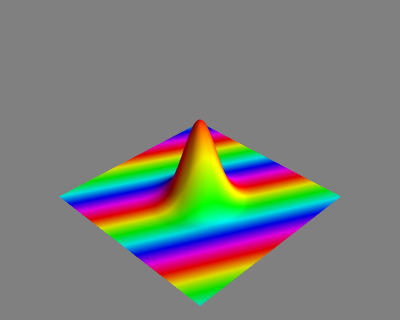
\includegraphics[width=0.5\linewidth]{./fig/phi/phi_0-0.png}
  }
  \subfloat[][]{
    \label{fig:phi_10}
    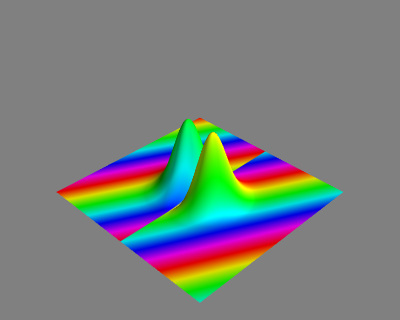
\includegraphics[width=0.5\linewidth]{./fig/phi/phi_1-0.png}
  } \\
  \subfloat[][]{
    \label{fig:phi_01}
    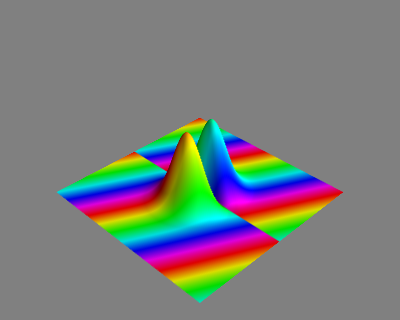
\includegraphics[width=0.5\linewidth]{./fig/phi/phi_0-1.png}
  }
  \subfloat[][]{
    \label{fig:phi_11}
    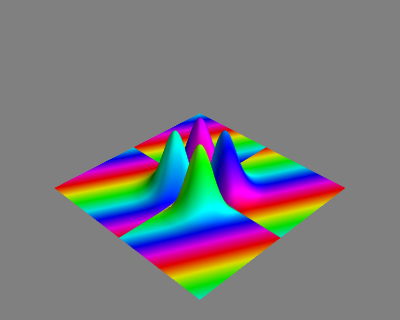
\includegraphics[width=0.5\linewidth]{./fig/phi/phi_1-1.png}
  } \\
  \subfloat[][]{
    \label{fig:phi_02}
    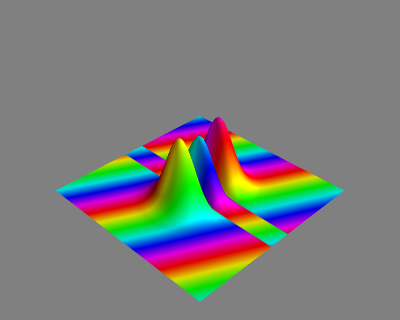
\includegraphics[width=0.5\linewidth]{./fig/phi/phi_0-2.png}
  }
  \subfloat[][]{
    \label{fig:phi_12}
    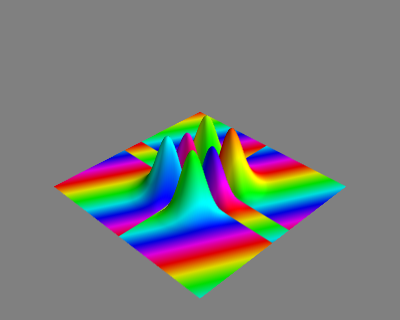
\includegraphics[width=0.5\linewidth]{./fig/phi/phi_1-2.png}
  } \\
  \caption[Plots of some basis functions $\phi$]{
    Plots of the first few functions $\phi_{k,l}$ with parameters set
    to $\vec{q} = \vec{0}$, $\vec{p} = (1, \frac{1}{2})$, $\mat{Q} = \id$, $\mat{P} = i \id$
    and $\varepsilon = 1$. The surface represents ten times the value
    $\sqrt{\Braket{\phi_{k,l}|\phi_{k,l}}}$ where the factor of $10$
    is just for visual purpose. For an explanation of the colours, see appendix \ref{ch:color_code}.
    \subref{fig:phi_00} $\phi_{0,0}$
    \subref{fig:phi_10} $\phi_{1,0}$
    \subref{fig:phi_01} $\phi_{0,1}$
    \subref{fig:phi_11} $\phi_{1,1}$
    \subref{fig:phi_02} $\phi_{0,2}$
    \subref{fig:phi_12} $\phi_{1,2}$
    \label{fig:phi_table_1}
  }
\end{figure}


\begin{figure}
  \centering
  \subfloat[][]{
    \label{fig:phi_20}
    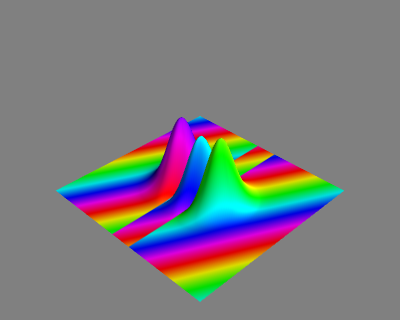
\includegraphics[width=0.5\linewidth]{./fig/phi/phi_2-0.png}
  }
  \subfloat[][]{
    \label{fig:phi_30}
    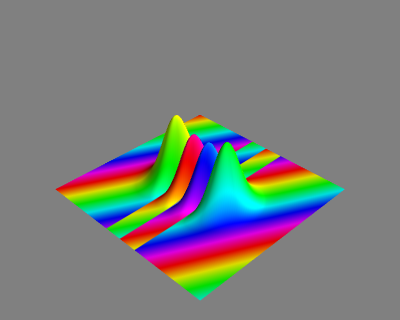
\includegraphics[width=0.5\linewidth]{./fig/phi/phi_3-0.png}
  } \\
  \subfloat[][]{
    \label{fig:phi_21}
    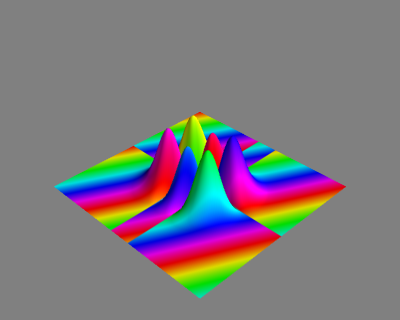
\includegraphics[width=0.5\linewidth]{./fig/phi/phi_2-1.png}
  }
  \subfloat[][]{
    \label{fig:phi_31}
    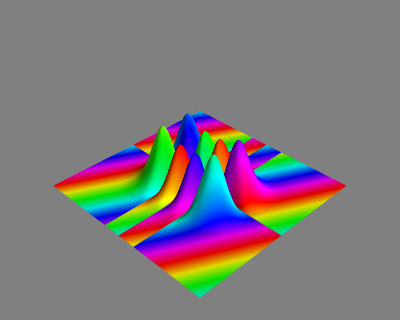
\includegraphics[width=0.5\linewidth]{./fig/phi/phi_3-1.png}
  } \\
  \subfloat[][]{
    \label{fig:phi_22}
    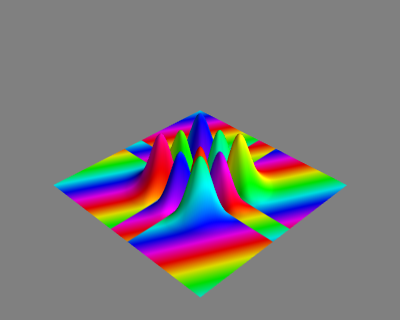
\includegraphics[width=0.5\linewidth]{./fig/phi/phi_2-2.png}
  }
  \subfloat[][]{
    \label{fig:phi_32}
    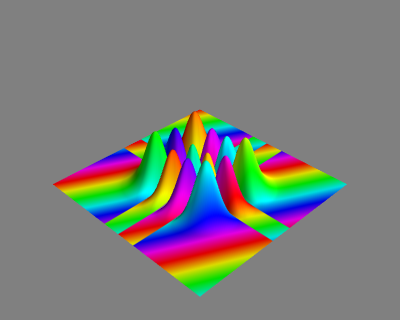
\includegraphics[width=0.5\linewidth]{./fig/phi/phi_3-2.png}
  } \\
  \caption[Plots of some basis functions $\phi$]{
    Plots of the first few functions $\phi_{k,l}$ with parameters set
    to $\vec{q} = \vec{0}$, $\vec{p} = (1, \frac{1}{2})$, $\mat{Q} = \id$, $\mat{P} = i \id$
    and $\varepsilon = 1$. The surface represents ten times the value
    $\sqrt{\Braket{\phi_{k,l}|\phi_{k,l}}}$ where the factor of $10$
    is just for visual purpose. For an explanation of the colours, see appendix \ref{ch:color_code}.
    \subref{fig:phi_20} $\phi_{2,0}$
    \subref{fig:phi_30} $\phi_{3,0}$
    \subref{fig:phi_21} $\phi_{2,1}$
    \subref{fig:phi_31} $\phi_{3,1}$
    \subref{fig:phi_22} $\phi_{2,2}$
    \subref{fig:phi_32} $\phi_{3,2}$
    \label{fig:phi_table_2}
  }
\end{figure}


\section{Construction of wavepackets}


In the previous section we saw how to compute the functions $\phi_{\vec{k}}[\Pi](\vec{x})$.
Now we can take a very general set $\mathfrak{K}$ of indices $\vec{k}$ and use
the corresponding functions $\phi_{\vec{k}}$ to build a (more or less truncated)
basis for $L^2(\mathbb{R}^D)$. In a first step we can construct so called
\emph{scalar wavepackets} $\Phi$ by linear combinations:

\begin{equation}
  \Phi(\vec{x}) \assign \exp\left(\frac{i S}{\varepsilon^2}\right) \sum_{\vec{k}\in\mathfrak{K}} c_{\vec{k}} \phi_{\vec{k}}
\end{equation}

where the coefficients $c_{\vec{k}} \in \mathbb{C}$ depend on time only and the basis functions
$\phi_{\vec{k}}$ depend on space but also on time through the parameter set
$\Pi(t)$ which is time-dependent\footnote{In general we neglect explicit
time-dependence of the parameter set $\Pi$ in our notation.}. We added a global
phase $S$ which is also time-dependent. An overly precise notation reads:

\begin{definition}[Scalar semi-classical wavepacket]
  \begin{equation} \label{eq:scalar_wavepacket}
    \Ket{\Phi} \assign
    \Phi\left[\Pi(t)\right](\vec{x}, t)
    =
    \exp\left(\frac{i S(t)}{\varepsilon^2}\right) \sum_{\vec{k}\in\mathfrak{K}} c_{\vec{k}}(t) \phi_{\vec{k}}\left[\Pi(t)\right](\vec{x}) \,.
  \end{equation}
\end{definition}

Every single basis function $\phi_{\vec{k}}$ is a perfectly valid wavepacket too.
Sometimes we will append the parameter $S$ to the set $\Pi$ and use the notation
$\Pi = \{q,p,Q,P,S\}$. This should be clear from the context. Also we will drop
the time variable since we look at wavepackets at fixed times.


\section{Basis set expansion and basis shapes}


The above formulation is a basis expansion for the true wavefunction $\varphi(\vec{x}, t)$.
Remember that the set $\{\phi_{\vec{k}}\}_{\vec{k}\in\mathfrak{K}}$ is a (complete)
basis of the function space $L^2(\mathbb{R}^D)$. Hence the basis expansion is
exact if we take the full lattice $\mathfrak{K} = \mathbb{N}_0^D$ of indices. In
theoretical considerations we can use the full lattice but for all practical
purposes we need to truncate the basis and make the set $\mathfrak{K}$ finite.
This can be done in various ways and we refer to the \emph{shape} of a basis set
if we speak about these details of $\mathfrak{K}$. Basis shapes usually depend
on some parameters $\theta$, we occasionally write $\mathfrak{K}(\theta)$ for this.

For a first ansatz we can use a hypercubic basis set $\mathfrak{K}$ which means
that we take the subset of all lattice points for which $\vec{k} < \vec{K}$ holds.
The components of $\vec{K}$ specify the number of points along each of the $D$
directions. A more formal definition is:

\begin{definition}[Hypercubic basis shape]
  \begin{equation}
    \mathfrak{K}(\vec{K}) \assign \left\{ \vec{k} \in \mathbb{N}_0^D :
                                          \, k_d < K_d \,\forall\, d \in [0, \ldots, D-1] \right\} \,.
  \end{equation}
\end{definition}

If we use this basis shape we call the resulting wavepacket \emph{dense}. By
$|\mathfrak{K}|$ we denote the \emph{basis size}, the overall number of basis
functions $\phi_{\vec{k}}$ we use. In the hypercubic case this is obviously:

\begin{equation}
  |\mathfrak{K}| = \prod_{d=0}^{D-1} K_d \,.
\end{equation}

As a shorthand notation to specify the hypercubic shape we simply write
$\mathfrak{K} = \vec{K} = [K_0, \ldots, K_{D-1}]$. We should think of $\vec{K}$ as
being both the vector in the lattice $\mathbb{N}_0^D$ and the set of all index
points in the hypercube spanned by the origin $\vec{0} = (0, \ldots, 0)$ and
$\vec{K} - \vec{1} = (K_0-1, \ldots, K_{D-1}-1)$, depending on the context.

The size of this basis shape grows exponentially with the number $D$ of dimensions.
Therefore we introduce more sparse basis sets which grow slower as the number
of dimensions increases. The first example is the \emph{hyperbolic cut} basis shape
defined as follows:

\begin{definition}[Hyperbolic cut basis shape] \label{def:hyperbolic_cut_shape}
  \begin{equation}
    \mathfrak{K}(K) \assign \left\{ \vec{k} \in \mathbb{N}_0^D :
                                    \, \prod_{d=0}^{D-1}(1+k_d) \leq K \right\}
  \end{equation}
\end{definition}

where we limit the number of basis functions by hyperbolic cuts. For this we
introduce a scalar parameter $K \in \mathbb{N}$ which we call \emph{sparsity}
in this context. The number of basis functions is then bounded by:

\begin{equation}
  |\mathfrak{K}| \leq \mathcal{C} K \left(\log K\right)^{D-1} \,.
\end{equation}

where $\mathcal{C}$ is some constant.

Figure \ref{fig:hyperbolic_cut_basis_size} shows the application of this bound
to the two-dimensional case.

\begin{figure}
  \centering
  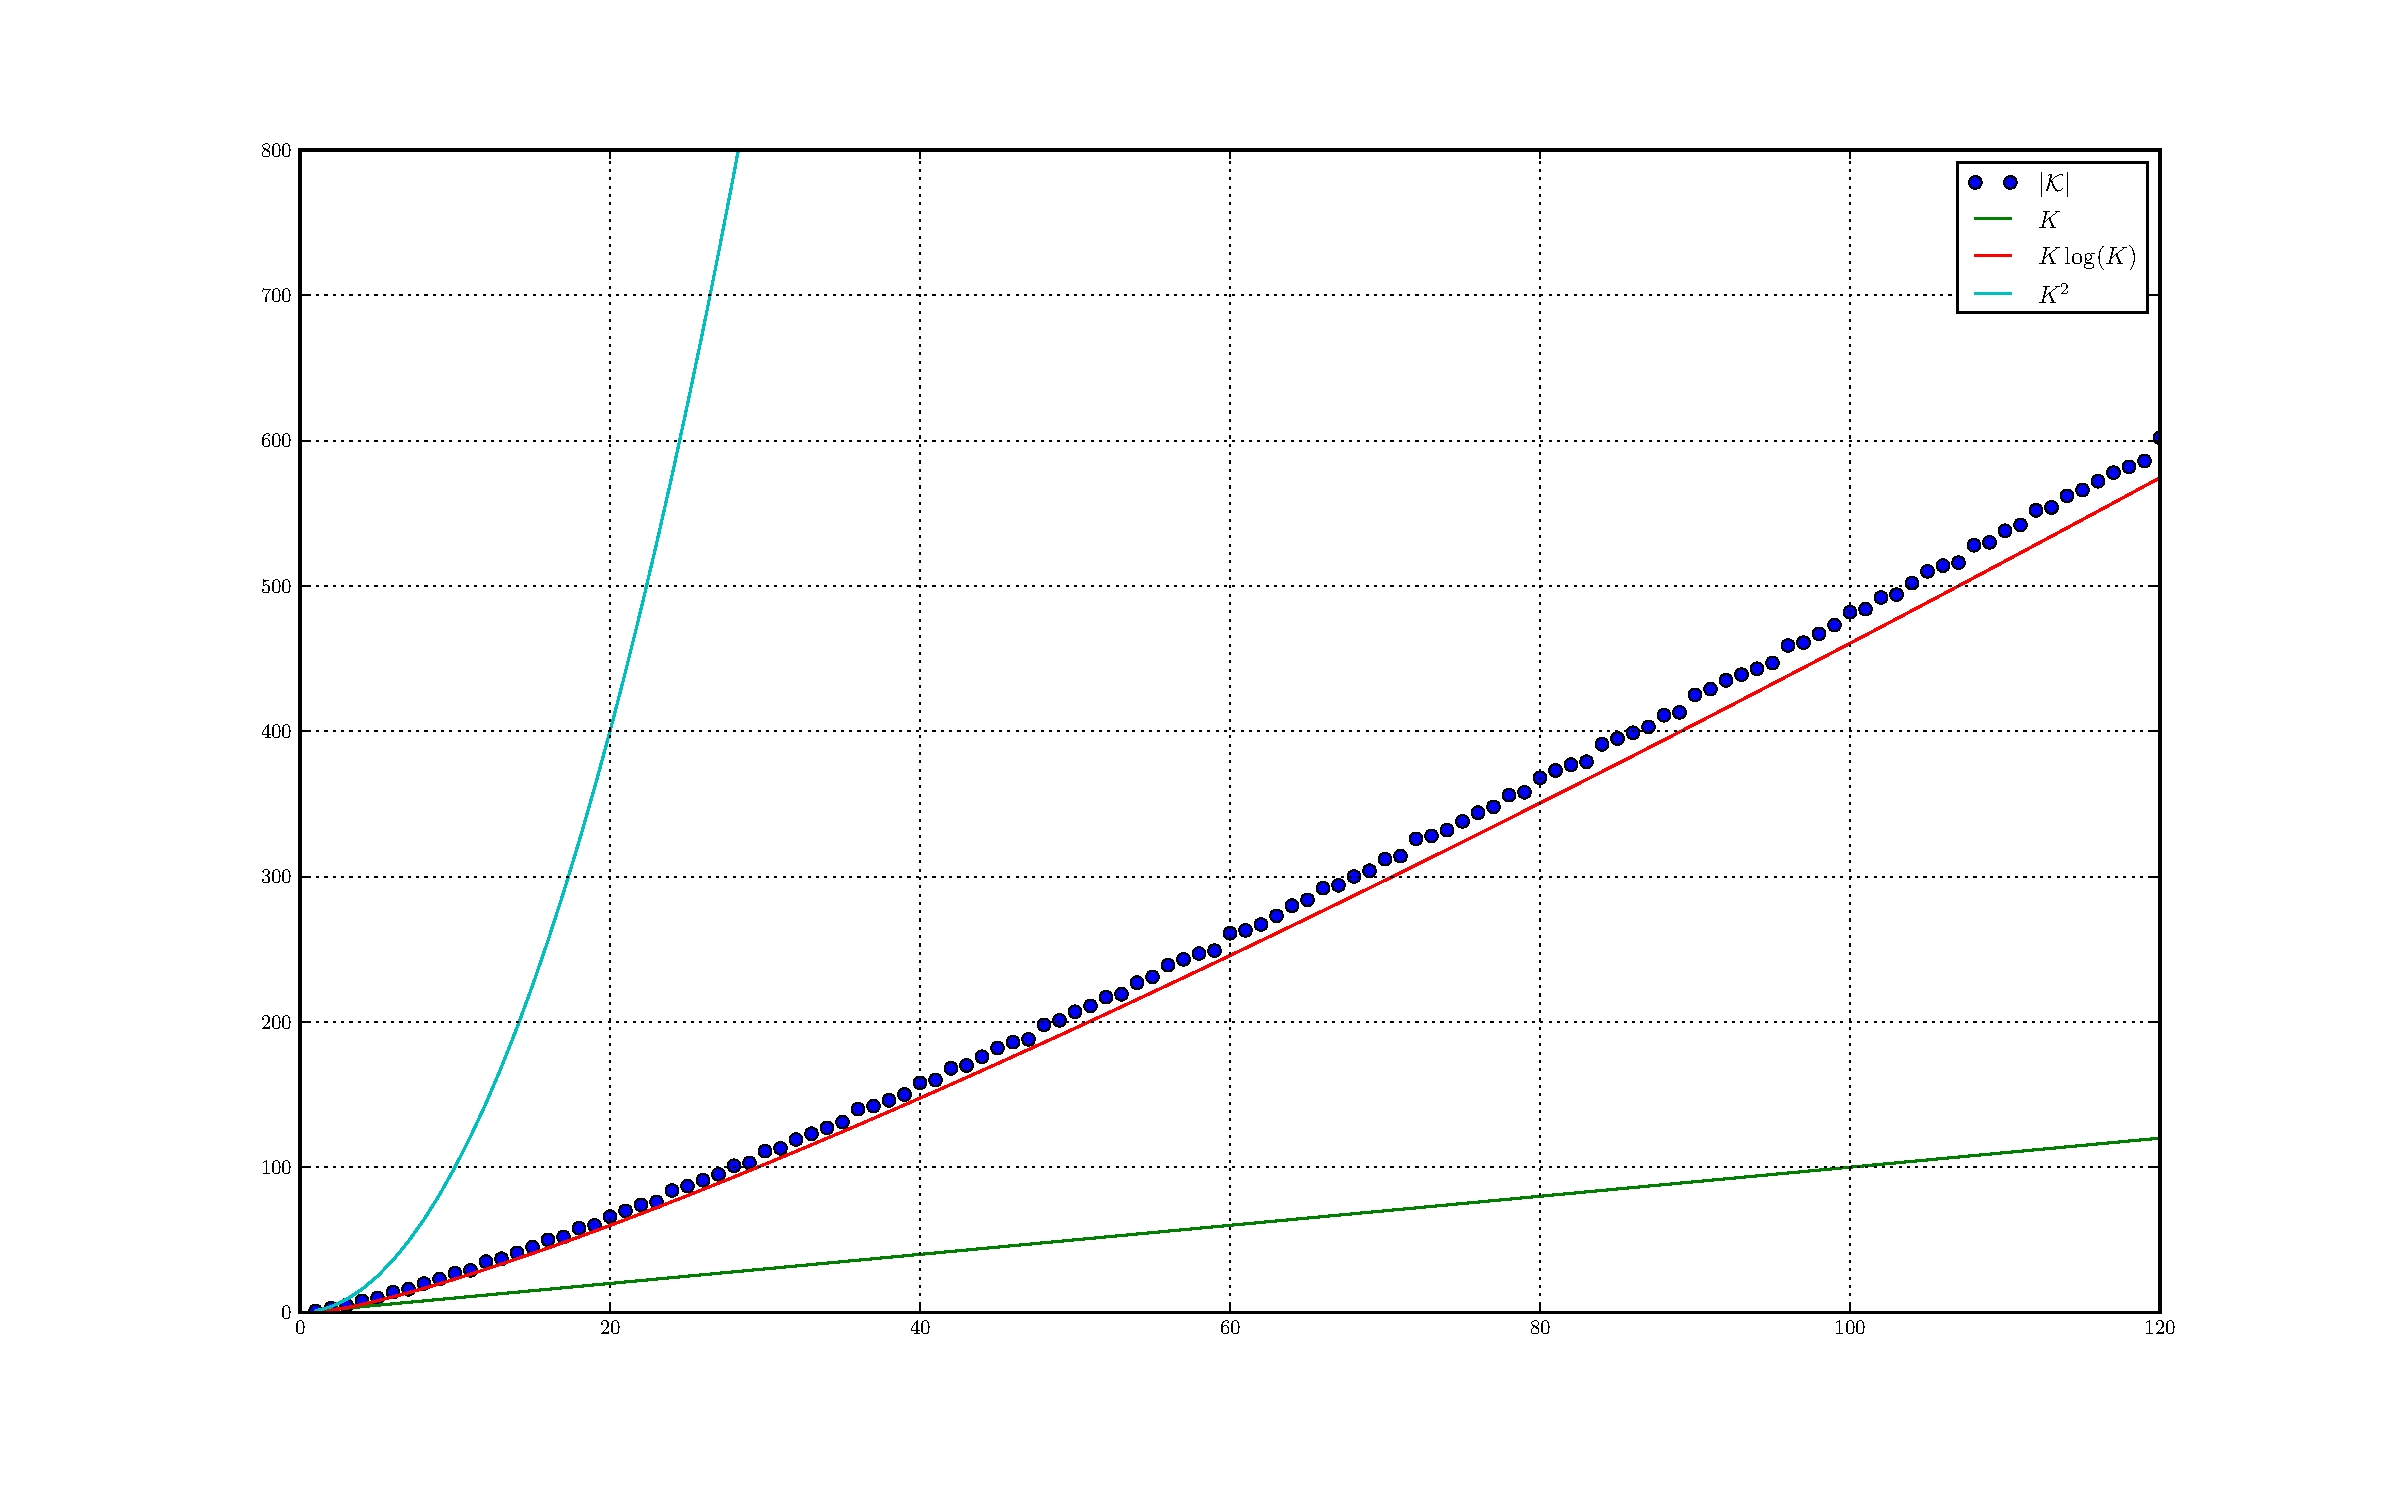
\includegraphics[width=0.8\linewidth]{./fig/basis_size.pdf}
  \caption{The size $|\mathfrak{K}|$ of two-dimensional hyperbolic basis shapes
           with various cut-off values $K$.}
  \label{fig:hyperbolic_cut_basis_size}
\end{figure}

\begin{figure}
  \centering
  \subfloat[][]{
    \label{fig:hyperbolic_cut_2_8}
    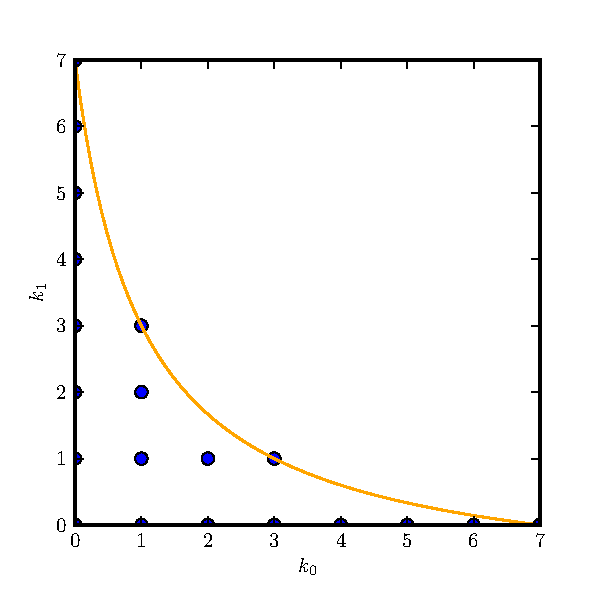
\includegraphics[width=0.5\linewidth]{./fig/hyperbolic_shape_2_8.pdf}
  }
  \subfloat[][]{
    \label{fig:hyperbolic_cut_2_32}
    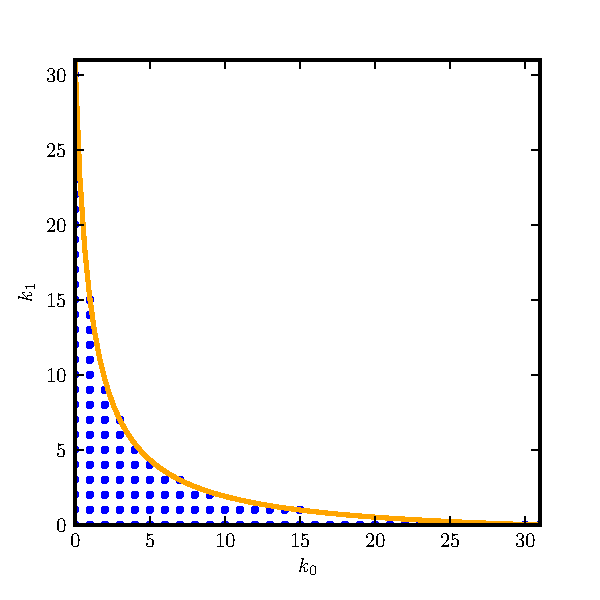
\includegraphics[width=0.5\linewidth]{./fig/hyperbolic_shape_2_32.pdf}
  } \\
  \caption[Hyperbolic cut basis shape in two dimensions]{
    The lattice nodes that are part of a two-dimensional hyperbolic cut basis
    shape. Additionally the cut-off function is shown. Compared to the full
    hypercubic basis shape the sparsity of this type of basis shape becomes
    clearly visible.
    \subref{fig:hyperbolic_cut_2_8} $K = 8$
    \subref{fig:hyperbolic_cut_2_32} $K = 32$
    \label{fig:hyperbolic_cut_2D}
  }
\end{figure}

\begin{figure}
  \centering
  \subfloat[][]{
    \label{fig:hyperbolic_cut_3_8}
    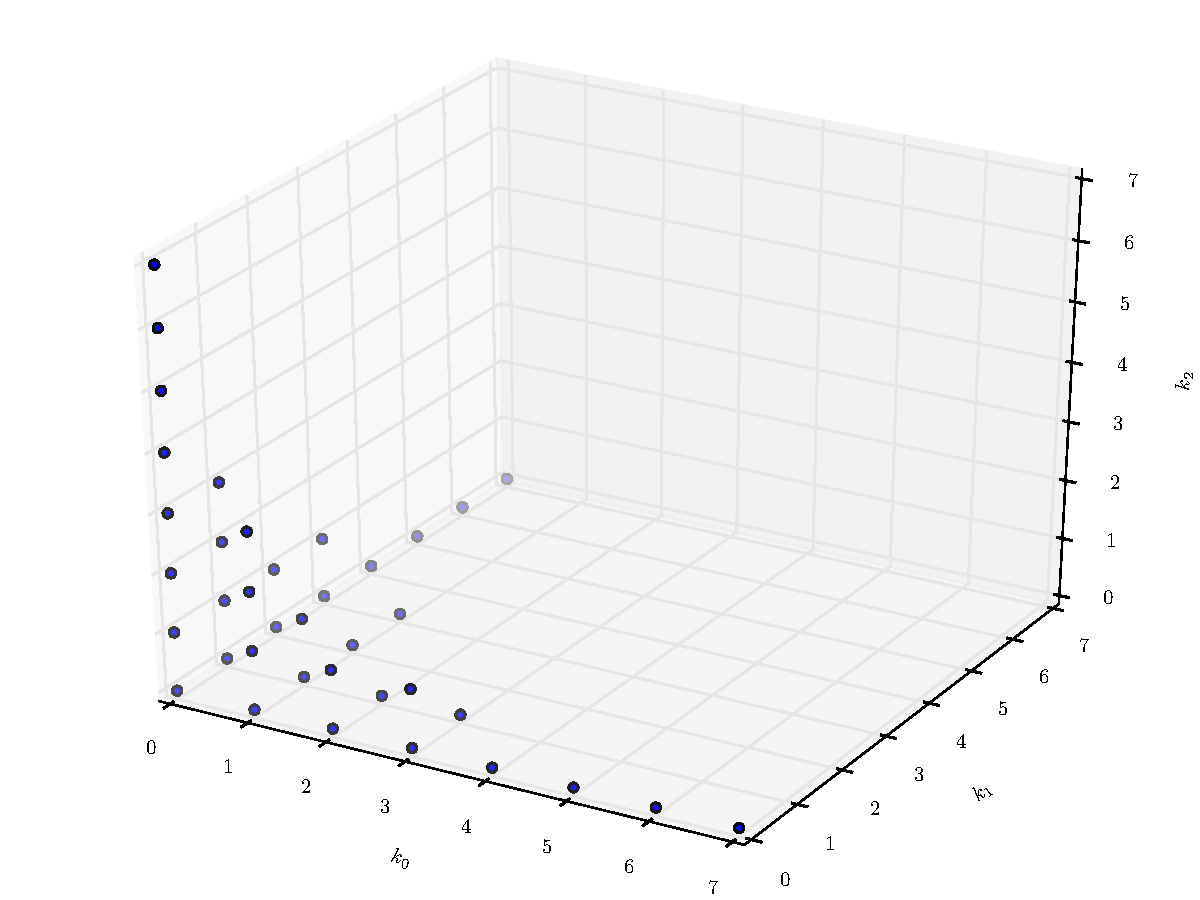
\includegraphics[width=0.5\linewidth]{./fig/hyperbolic_shape_3_8.pdf}
  }
  \subfloat[][]{
    \label{fig:hyperbolic_cut_3_32}
    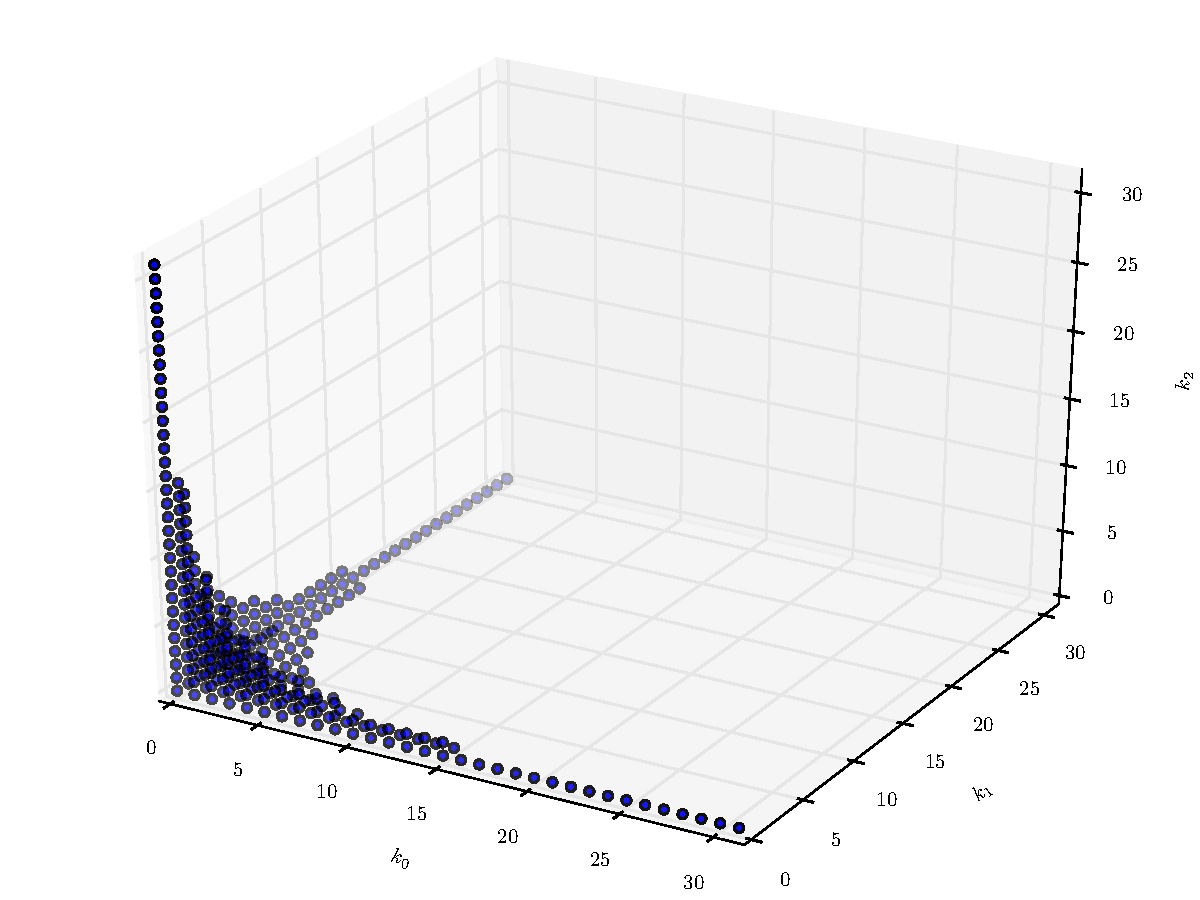
\includegraphics[width=0.5\linewidth]{./fig/hyperbolic_shape_3_32.pdf}
  } \\
  \caption[Hyperbolic cut basis shape in three dimensions]{
    The lattice nodes that are part of a three-dimensional hyperbolic cut basis
    shape. Compared to the full hypercubic basis shape the sparsity of this
    type of basis shape becomes clearly visible.
    \subref{fig:hyperbolic_cut_3_8} $K = 8$
    \subref{fig:hyperbolic_cut_3_32} $K = 32$
    \label{fig:hyperbolic_cut_3D}
  }
\end{figure}

As we see in figures \ref{fig:hyperbolic_cut_2D} and \ref{fig:hyperbolic_cut_3D}
this basis shape has long tails consisting of functions with high frequencies
in one direction. Sometimes we do not need these tails. We can combine the two
basis shapes introduced and define a new shape:

\begin{definition}[Hyperbolic cut basis shape with limits]
  \begin{equation}
    \mathfrak{K}(K, \vec{L}) \assign \left\{ \vec{k} \in \mathbb{N}_0^D :
                             \prod_{d=0}^{D-1}(1+k_d) \leq K
                             \land k_d < L_d \,\forall\, d \in [0,\ldots,D-1] \right\} \,.
  \end{equation}
\end{definition}

The parameter $K \in \mathbb{N}$ is again the sparsity defining the hyperbolic
cuts. The parameter $\vec{L}$ is a list of $D$ elements with each $L_d \in \mathbb{N}$.
These limits act as sharp upper bounds on the entries of $\vec{k}$. In that way
we can combine the two previous basis shapes. If we choose $L_d \geq K \,\forall\,
d \in [0,\ldots, D-1]$ then we obtain a simple hyperbolic cut basis shape. On the
other hand, if we set $K \geq \prod_{d=0}^{D-1} L_d$ we are back in the full
hypercubic case.

\begin{figure}
  \centering
  \subfloat[][]{
    \label{fig:hyperbolic_limited_2_8}
    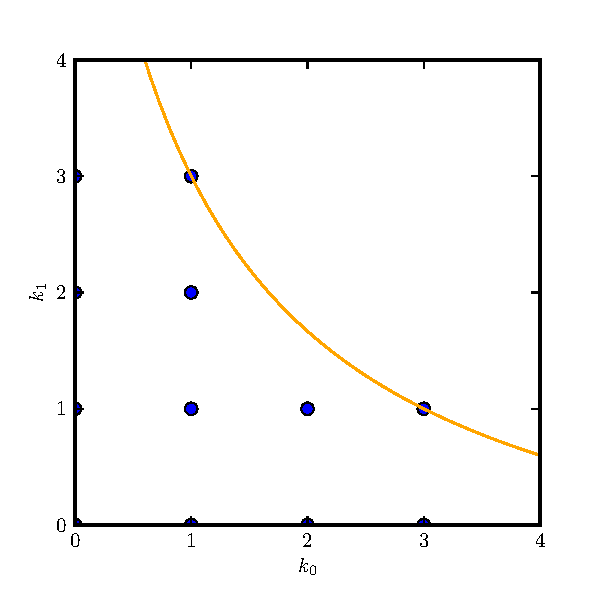
\includegraphics[width=0.5\linewidth]{./fig/hyperbolic_limited_2_8.pdf}
  }
  \subfloat[][]{
    \label{fig:hyperbolic_limited_2_32}
    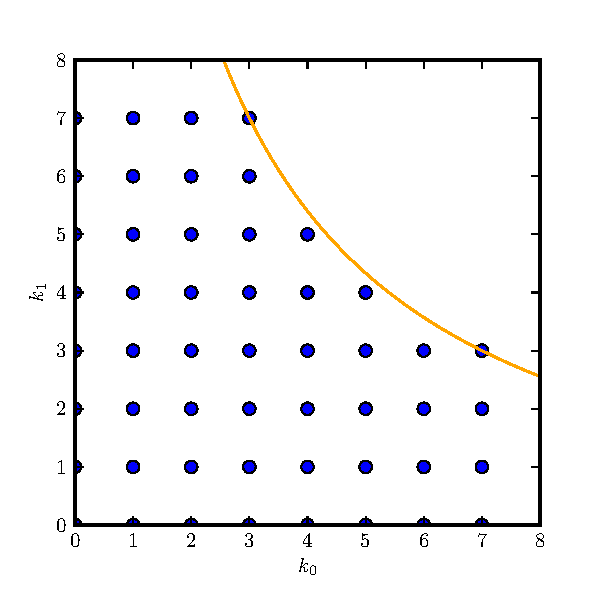
\includegraphics[width=0.5\linewidth]{./fig/hyperbolic_limited_2_32.pdf}
  } \\
  \caption[Hyperbolic cut basis shape with limits in two dimensions]{
    The lattice nodes that are part of a two-dimensional limited hyperbolic cut
    basis shape. Compared to the unlimited hyperbolic cut basis shape
    the long tails are missing here.
    \subref{fig:hyperbolic_limited_2_8} $K = 8$ and $\vec{L} = (4,4)$
    \subref{fig:hyperbolic_limited_2_32} $K = 32$ and $\vec{L} = (8,8)$
    \label{fig:hyperbolic_limited_2D}
  }
\end{figure}

There exist many more possibilities for specific basis shapes. For a generic
basis shape $\mathfrak{K}$ a fundamental property has to hold. We can state
it by the following implication:

\begin{equation}
  \forall\, \vec{k} \in \mathbb{N}_0^D:
  \vec{k} \in \mathfrak{K} \Rightarrow \vec{k} - \vec{e}^d \in \mathfrak{K} \,\forall\, d \in [0, \ldots, D-1] \,.
\end{equation}

% \begin{equation}
%   \mathfrak{K} := \left\{ \vec{k} \in \mathbb{N}_0^D :
%                           \vec{k} - \vec{e}^d \in \mathfrak{K} \,\forall\, d \in [0, \ldots, D-1] \right\} \,.
% \end{equation}

In other words, for each $\vec{k} \in \mathfrak{K}$ it must hold that for all
$d = 0, \ldots, D-1$ the multi-index defined by $k^\prime \assign \vec{k} - \vec{e}^d$
has no negative components and $\vec{k}^\prime \in \mathfrak{K}$. In less formal
terms this means that an index $\vec{k}$ is part of $\mathfrak{K}$ iff all its
backward neighbours are also part of $\mathfrak{K}$. This condition is necessary
for the recursive evaluation of wavepackets which we will show later.

Probably the most general way to write a scalar wavepacket \eqref{eq:scalar_wavepacket}
now is:

\begin{equation}
  \Ket{\Phi} \assign
  \Phi\left[\Pi(t), \mathfrak{K}(t)\right](\vec{x}, t)
  =
  \exp\left(\frac{i S(t)}{\varepsilon^2}\right) \sum_{\vec{k}\in\mathfrak{K}(t)} c_{\vec{k}}(t) \phi_{\vec{k}}\left[\Pi(t)\right](\vec{x})
\end{equation}

which uses an arbitrary, possibly time-adaptive basis shape $\mathfrak{K}(t)$. In
principle we can exchange the basis shapes at each timestep during the simulation.
This provides us with adaptivity for all parameters $\theta$ a basis shape depends on.

Sometimes we will need to bring the elements $\vec{k}$ of a basis shape $\mathfrak{K}$
into a fixed total order. This is done by the \emph{linearisation mapping}.

\begin{definition}[Linearisation mapping]
  A mapping:
  \begin{align*}
    \mu : \mathfrak{K} & \rightarrow \mathbb{N}_0 \\
          \vec{k}      & \mapsto     n
  \end{align*}
  that fixes a total order of the set $\mathfrak{K}$.
\end{definition}

If it is not clear from the context we denote this mapping by $\mu_{\mathfrak{K}}$
to mark explicitly which basis shape it belongs to. In practical cases we usually
have $\mu(\vec{0}) = 0$ but this is not a requirement.

Finally the following two algorithms \ref{al:forward_neighbours} and
\ref{al:backward_neighbours} can be used to find the neighbourhood
of a given multi-index $\vec{k}$ in a general basis shape $\mathfrak{K}$.

\begin{algorithm}
  \caption{Find forward neighbours}
  \label{al:forward_neighbours}
  \begin{algorithmic}
    \REQUIRE The number $D$ of space dimensions
    \REQUIRE The basis shape $\mathfrak{K}$
    \REQUIRE The multi-index $\vec{k}$ whose neighbours we search

    \STATE // List for the result
    \STATE $N \assign \{\}$
    \STATE // Find neighbourhood
    \FOR{$d = 0$ \TO $d = D-1$}
      \STATE $\vec{k}^\prime \assign \vec{k} + \vec{e}^d$
      \IF{$\vec{k}^\prime \in \mathfrak{K}$}
        \STATE $N = N \cup \{(\vec{k}^\prime, d)\}$
      \ENDIF
    \ENDFOR

    \RETURN $N$
  \end{algorithmic}
\end{algorithm}

\begin{algorithm}
  \caption{Find backward neighbours}
  \label{al:backward_neighbours}
  \begin{algorithmic}
    \REQUIRE The number $D$ of space dimensions
    \REQUIRE The basis shape $\mathfrak{K}$
    \REQUIRE The multi-index $\vec{k}$ whose neighbours we search

    \STATE // List for the result
    \STATE $N \assign \{\}$
    \STATE // Find neighbourhood
    \FOR{$d = 0$ \TO $d = D-1$}
      \STATE $\vec{k}^\prime \assign \vec{k} - \vec{e}^d$
      \IF{$\vec{k}^\prime \in \mathfrak{K}$}
        \STATE $N = N \cup \{(\vec{k}^\prime, d)\}$
      \ENDIF
    \ENDFOR

    \RETURN $N$
  \end{algorithmic}
\end{algorithm}


\subsection{Basis shape transformation mappings}


Given two basis shapes $\mathfrak{K}$ and $\mathfrak{K}^\prime$ and their
linearisation mappings:

\begin{align*}
  \mu: \mathfrak{K} & \rightarrow \mathbb{N}_0 \\
  \mu^\prime: \mathfrak{K}^\prime & \rightarrow \mathbb{N}_0 \,.
\end{align*}

We look for a way how to change a data array $\vec{c} \in \mathbb{C}^{|\mathfrak{K}|}$
(storing complex scalar data for each multi-index $\vec{k} \in \mathfrak{K}$
at the position $\vec{c}_{\mu(\vec{k})}$) if we replace the basis shape $\mathfrak{K}$
by $\mathfrak{K}^\prime$. The problem is that the two mappings are in general
incompatible with each other. Hence we have to permute the elements of the array $\vec{c}$.
Referring to figure \ref{fig:map}, the task is now to connect the keys $i$ and
$i^\prime$ such that for all multi-indices $\vec{k} \in \mathfrak{K} \cap \mathfrak{K}^\prime$
it holds that:

\begin{equation*}
  \left(\mu^\prime\right)^{-1} \left( T\left( \mu\left(\vec{k}\right) \right) \right) = \vec{k} \,.
\end{equation*}

The transformation $T$ is bijective if and only if
$\mathfrak{K} \equiv \mathfrak{K} \cap \mathfrak{K}^\prime \equiv \mathfrak{K}^\prime$.

\begin{figure}
  \centering
  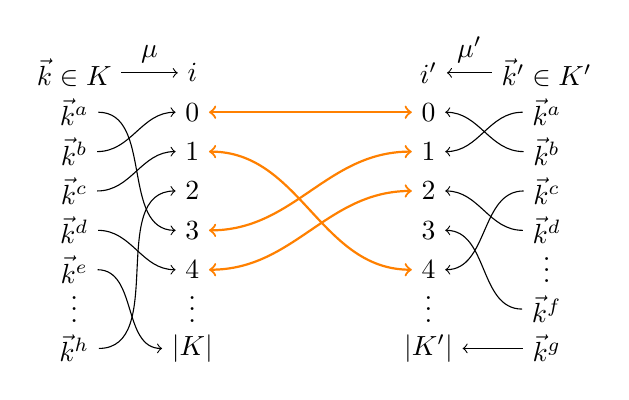
\begin{tikzpicture}[%
    node distance=0.5cm, auto,
    func/.style={scale=0.8,color=gray},
    zero/.style={scale=0.8,color=gray}]

    \node (ko) {$\vec{k} \in \mathfrak{K}$};
    \node (io) [right of=ko, node distance=1.5cm] {$i$};
    \draw[->] (ko) to node {$\mu$} (io);

    \node (ko0) [below of=ko] {$\vec{k}^a$};
    \node (ko1) [below of=ko0] {$\vec{k}^b$};
    \node (ko2) [below of=ko1] {$\vec{k}^c$};
    \node (ko3) [below of=ko2] {$\vec{k}^d$};
    \node (ko4) [below of=ko3] {$\vec{k}^e$};
    \node (ko5) [below of=ko4, node distance=4mm] {$\vdots$};
    \node (ko6) [below of=ko5, node distance=6mm] {$\vec{k}^h$};

    \node (io0) [below of=io] {$0$};
    \node (io1) [below of=io0] {$1$};
    \node (io2) [below of=io1] {$2$};
    \node (io3) [below of=io2] {$3$};
    \node (io4) [below of=io3] {$4$};
    \node (io5) [below of=io4, node distance=4mm] {$\vdots$};
    \node (io6) [below of=io5, node distance=6mm] {$|\mathfrak{K}|$};

    \draw[->] (ko0) to[out=0,in=180] node {} (io3);
    \draw[->] (ko1) to[out=0,in=180] node {} (io0);
    \draw[->] (ko2) to[out=0,in=180] node {} (io1);
    \draw[->] (ko3) to[out=0,in=180] node {} (io4);
    \draw[->] (ko4) to[out=0,in=180] node {} (io6);
    \draw[->] (ko6) to[out=0,in=180] node {} (io2);

    \node (ip) [right of=io, node distance=3cm] {$i^\prime$};
    \node (kp) [right of=ip, node distance=1.5cm] {$\vec{k}^\prime \in \mathfrak{K}^\prime$};
    \draw[<-] (ip) to node {$\mu^\prime$} (kp);

    \node (kp0) [below of=kp] {$\vec{k}^a$};
    \node (kp1) [below of=kp0] {$\vec{k}^b$};
    \node (kp2) [below of=kp1] {$\vec{k}^c$};
    \node (kp3) [below of=kp2] {$\vec{k}^d$};
    \node (kp4) [below of=kp3, node distance=4mm] {$\vdots$};
    \node (kp5) [below of=kp4, node distance=6mm] {$\vec{k}^f$};
    \node (kp6) [below of=kp5] {$\vec{k}^g$};

    \node (ip0) [below of=ip] {$0$};
    \node (ip1) [below of=ip0] {$1$};
    \node (ip2) [below of=ip1] {$2$};
    \node (ip3) [below of=ip2] {$3$};
    \node (ip4) [below of=ip3] {$4$};
    \node (ip5) [below of=ip4, node distance=4mm] {$\vdots$};
    \node (ip6) [below of=ip5, node distance=6mm] {$|\mathfrak{K}^\prime|$};

    \draw[->] (kp0) to[out=180,in=0] node {} (ip1);
    \draw[->] (kp1) to[out=180,in=0] node {} (ip0);
    \draw[->] (kp2) to[out=180,in=0] node {} (ip4);
    \draw[->] (kp3) to[out=180,in=0] node {} (ip2);
    \draw[->] (kp5) to[out=180,in=0] node {} (ip3);
    \draw[->] (kp6) to[out=180,in=0] node {} (ip6);

    \draw[thick, <->, color=orange] (io0) to[out=0,in=180] node {} (ip0);
    \draw[thick, <->, color=orange] (io1) to[out=0,in=180] node {} (ip4);
    \draw[thick, <->, color=orange] (io3) to[out=0,in=180] node {} (ip1);
    \draw[thick, <->, color=orange] (io4) to[out=0,in=180] node {} (ip2);
\end{tikzpicture}

  \caption[Basis shape transformation mapping]
  {The two mappings $\mu$ and $\mu^\prime$ together with the transformation rule $T$ (orange arrows).}
  \label{fig:map}
\end{figure}

When remapping linearly indexed data vectors $\vec{c}_{\mu\left(\vec{k}\right)}$,
we drop the entries for all $\vec{k} \in \mathfrak{K} \setminus \mathfrak{K}^\prime$
and we fill in zero values for all $\vec{k} \in \mathfrak{K}^\prime \setminus \mathfrak{K}$.
The procedure is shown in algorithm \ref{al:basis_shape_remapping} below.

\begin{algorithm}
  \caption{Transformation of basis shapes and data remapping}
  \label{al:basis_shape_remapping}
  \begin{algorithmic}
    \REQUIRE The old basis shape $\mathfrak{K}$
    \REQUIRE The new basis shape $\mathfrak{K}^\prime$
    \REQUIRE An array $\vec{c}$ of length $|\mathfrak{K}|$ containing arbitrary data
    \STATE // Set up the new array of length $|\mathfrak{K}^\prime|$
    \STATE $\vec{c}^\prime \assign \vec{0} \in \mathbb{C}^{|\mathfrak{K}^\prime|}$
    \STATE // Copy over the data we can keep
    \FOR{$\vec{k} \in \mathfrak{K} \cap \mathfrak{K}^\prime$}
      \STATE // Compute linear mapping of $\vec{k}$ in both basis shapes
      \STATE $i \assign \mu\left(\vec{k}\right)$
      \STATE $j \assign \mu^\prime\left(\vec{k}\right)$
      \STATE // Update the array
      \STATE $\vec{c}^\prime\left[j\right] = \vec{c}\left[i\right]$
    \ENDFOR
  \end{algorithmic}
\end{algorithm}

An example of such a mapping is given in figure \ref{fig:trafo_map}.

\begin{figure}
  \centering
  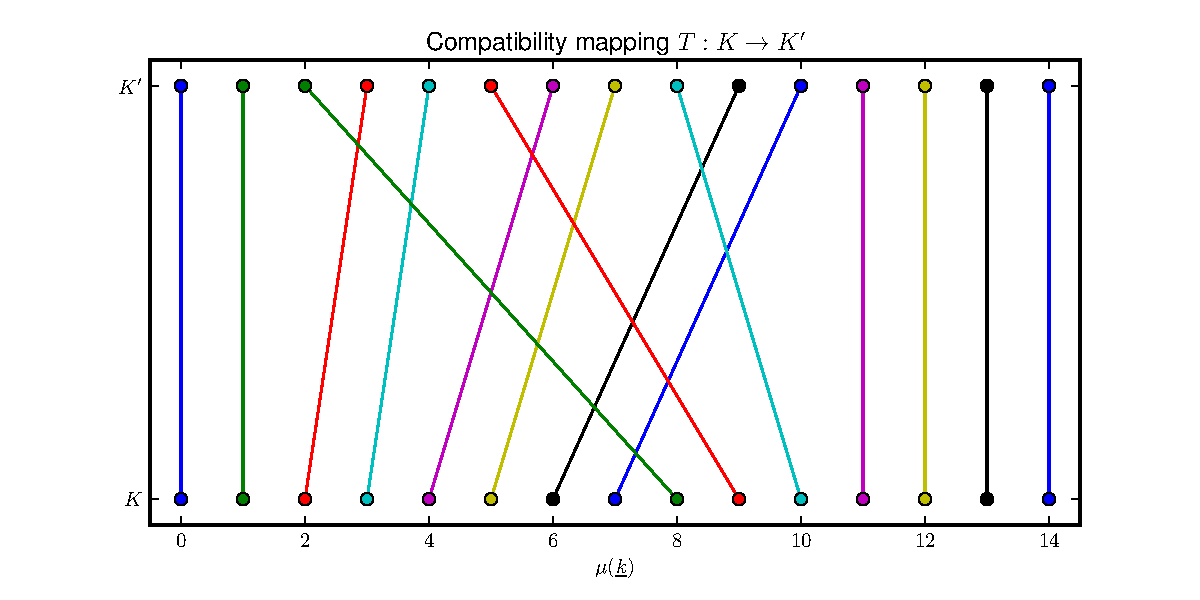
\includegraphics[scale=0.5]{./fig/trafo_map.pdf}
  \caption[Transformation mapping example]
          {An example of a basis shape transformation mapping $T$. The original
          shape was $\mathfrak{K} = \vec{K} = (4,2)$ and $|\mathfrak{K}| = 8$ while
          the new shape is $\mathfrak{K}^{\prime} = \vec{K}^{\prime} = (5,3)$ and
          $|\mathfrak{K}^{\prime}| = 15$.}
  \label{fig:trafo_map}
\end{figure}


\subsection{Basis shape extensions}


For computing the gradients of wavepackets (see section \ref{sec:gradient_computation})
we need to extend the basis shape. Informally spoken, extending a basis shape
means that we add a node in each direction. For each lattice point of a shape
we add all its neighbours. A formal definition is:

\begin{definition}[Basis shape extension]
  Given a basis shape $\mathfrak{K}$ we define its extension $\overline{\mathfrak{K}}$ by:
  \begin{equation*}
    \overline{\mathfrak{K}} \assign \mathfrak{K}
                            \cup \left\{ \vec{k}^\prime : \vec{k}^\prime = \vec{k} + \vec{e}^d \,\forall\, d \in [0,\ldots,D-1]
                                                          \,\forall\, \vec{k} \in \mathfrak{K} \right\} \,.
  \end{equation*}
  This defines the most tight extension. But any even larger basis shape is a
  valid extension too. In any case it holds that $\mathfrak{K} \subset \overline{\mathfrak{K}}$.
\end{definition}

This definition is not handy enough to work with. For some of the less complex basis
shapes $\mathfrak{K}(\theta)$ it is often possible to express the extended shape
$\overline{\mathfrak{K}(\theta^\prime)}$ simply by modifying the parameters
$\theta$ the shape depends on.

If we look at a hypercubic basis shape $\mathfrak{K}(\vec{K})$ then we can express
its extension $\overline{\mathfrak{K}(\vec{K}^\prime)}$ by the new parameters
$\vec{K}^\prime$ which obviously are:

\begin{equation} \label{eq:extend_hypercubic}
  \vec{K}^\prime = [ K_0 + 1, \ldots, K_{D-1} +1 ] \,.
\end{equation}

The attentive reader may notice that in case $D > 1$ this new basis
includes one node too much, namely the lattice point $(K_0, \ldots, K_{D-1})$.
This however poses no problems beside wasting a very small amount of memory.
A basis shape extension has not to be tight with respect to the above definition.

For the hyperbolic cut shape, extension is less trivial. Assume that the sparsity is $K$.
We first look at the extension of a two-dimensional shape. Here the two nodes
$(K-1, 0)$ and $(0, K-1)$ are the outermost ones. Since the whole basis shape is
symmetric under permutation of the axes, we focus only on $(K-1, 0)$ lying on the first
axis. We have to make sure that its neighbours are part of $\overline{\mathfrak{K}}$.
This is guaranteed (by definition \ref{def:hyperbolic_cut_shape}) if we can
construct a new hyperbolic cut shape $\mathfrak{K}^\prime(K^\prime)$ that
contains the node $(K-1,1)$. By using the equation of the above definition we get:

\begin{equation*}
  (1+K-1)(1+1) \leq K^\prime
\end{equation*}

which we can solve for the minimal $K^\prime$ and find that:

\begin{equation} \label{eq:extend_hyperbolic_cut_1D}
  K^\prime = 2 K \,.
\end{equation}

In the general case of $D>1$ dimensions we have a similar equation:

\begin{align*}
  (1+K-1)(1+1)\cdots(1+1) & = (1+K-1)\left(\prod_{d=1}^{D-1}(1+1)\right) \leq K^\prime
\end{align*}

from which we obtain:

\begin{equation} \label{eq:extend_hyperbolic_cut_DD}
  K^\prime = 2^{D-1} K \,.
\end{equation}

This is only valid for $D>1$ and gives for $D=1$ the wrong result $K^\prime = K$.
If we want a single formula valid for all dimensions then we have to start from
the point $\vec{k} = (K, 0, \ldots, 0)$. For this point we get:

\begin{align*}
  (1+K)\left(\prod_{d=1}^{D-1}(1+1)\right) \leq K^\prime
\end{align*}

giving:

\begin{equation} \label{eq:extend_hyperbolic_cut_general}
  K^\prime = 2^{D-1} (K+1) \,.
\end{equation}

However we should note that this leads to overly big extensions for $D>1$
compared to the other formula. For example if we start with a two-dimensional
basis shape with $K=4$ then we get $K^\prime = 8$ and $K^\prime = 10$ respectively.
The basis sizes of the extended shapes are then $20$ and $27$ and the tight extension
given by the direct definition would have size $14$ but is not of hyperbolic
cut type.

Extending a hyperbolic cut basis shape with limits is easy again. First we change
the limits $\vec{L}$ according to \eqref{eq:extend_hypercubic}. Then we increase $K$
by using one of the formulae \eqref{eq:extend_hyperbolic_cut_1D} or
\eqref{eq:extend_hyperbolic_cut_DD} depending on the dimensionality.
That is all we need to do for this type of basis shape.

We can use the limited hyperbolic cut basis shape to produce more tight extensions
of the standard hyperbolic cut basis shapes. For an example, refer to figure
\ref{fig:hyperbolic_extensions_compared}.

\begin{figure}
  \centering
  \subfloat[][]{
    \label{fig:hyperbolic_extension}
    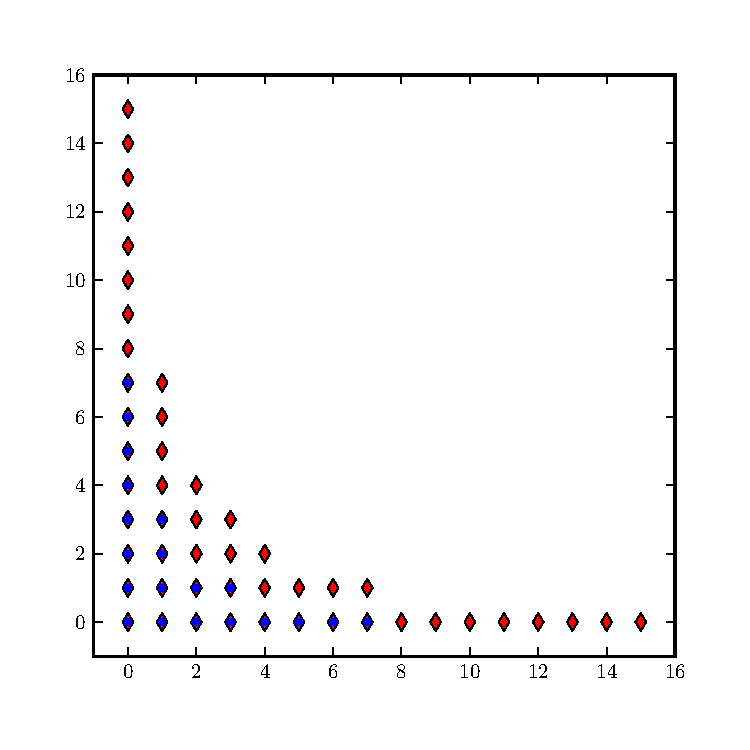
\includegraphics[width=0.5\linewidth]{./fig/hyperbolic_extension.pdf}
  }
  \subfloat[][]{
    \label{fig:hyperbolic_limited}
    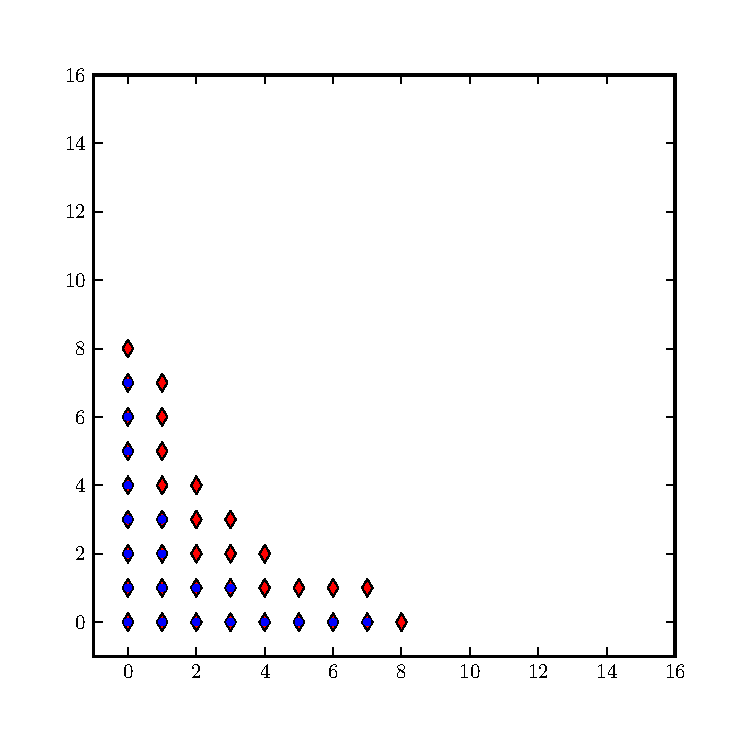
\includegraphics[width=0.5\linewidth]{./fig/hyperbolic_extension_limited.pdf}
  } \\
  \caption[Extensions of a hyperbolic cut basis shape]{
    Comparison of two methods to extend a hyperbolic cut basis shape with $K=8$.
    The original nodes (blue circles) and the nodes of the extension (red diamonds)
    are shown for both methods. The difference in basis size is $14$ nodes.
    \subref{fig:hyperbolic_extension} Extension is again an unlimited hyperbolic
                                      cut shape with $K = 16$.
    \subref{fig:hyperbolic_limited} Extension is a limited hyperbolic cut shape
                                    with $K = 16$ and $\vec{L} = (9,9)$. This extension
                                    introduces only $3$ nodes more than required.
    \label{fig:hyperbolic_extensions_compared}
  }
\end{figure}


\section{Evaluation of wavepackets}


For the numerical simulation we will need to evaluate a wavepacket at sets of
grid nodes $\vec{\gamma} \in \mathbb{R}^D$. The formula for the ground state
\eqref{eq:phi0_Dd} and the recursion \eqref{eq:basis_recursion_DD} for higher
order basis functions is in principle all we need to do this. Even if this
seems to be very simple at first glance there are a few tricky details involved.
In this section we start from the mathematical formulae and work towards an
algorithmic description for computing $\Phi(\vec{\gamma})$.

First we can evaluate the ground state $\phi_{\vec{0}}$ directly by algorithm \ref{al:eval_phi0_DD}.
If this is programmed by using vectorisation for the linear algebra functions we
can even perform the evaluation on a set $\Gamma = \{\gamma_i\}_i$ of nodes simultaneously.
The return value is then not a single scalar value but an array of scalars.
Usually we imagine this to be a row vector of $|\Gamma|$ elements.

\begin{algorithm}
\caption{Evaluate the ground state $\phi_0$ directly}
\label{al:eval_phi0_DD}
\begin{algorithmic}
  \REQUIRE The number $D$ of space dimensions
  \REQUIRE The Hagedorn parameter set $\Pi = \{q,p,Q,P\}$
  \REQUIRE The semi-classical scaling parameter $\varepsilon$
  \REQUIRE The grid node $\vec{\gamma} \in \mathbb{R}^D$

  \STATE // Whether to include the problematic prefactor or not
  \IF{prefactor is True}
    \STATE $\alpha \assign (\pi\varepsilon^2)^{-\frac{D}{4}} (\det\mat{Q})^{-\frac{1}{2}}$
  \ELSE
    \STATE $\alpha \assign (\pi\varepsilon^2)^{-\frac{D}{4}}$
  \ENDIF

  \STATE // The exponent
  \STATE $\vec{u} \assign \vec{\gamma}-\vec{q}$
  \STATE $\beta_1 \assign \dotp{\vec{u}}{\mat{P}\mat{Q}\inv\vec{u}}$
  \STATE $\beta_2 \assign \dotp{\vec{p}}{\vec{u}}$

  \STATE // The full ground state
  \STATE $\phi_{\vec{0}} \assign \alpha \exp\left(\frac{i}{\varepsilon^2}\left(\frac{1}{2}\beta_1 + \beta_2\right)\right)$

  \RETURN $\phi_{\vec{0}}$
\end{algorithmic}
\end{algorithm}

For the higher order basis functions $\phi_{\vec{k}}$ we employ the recursion
formula. With the help of this relation we can compute any $\phi_{\vec{k}}$
given some of the predecessors. For $D=1$ this is easy since we just compute
$\phi_{k+1}$ from $\phi_k$ and $\phi_{k-1}$. In the multi-dimensional case
it is less obvious what happens. To compute the set of all successors $\{\phi_{\vec{k}+\vec{e}^d}\}_{d=0}^{D-1}$
we need the function $\phi_{\vec{k}}$ as well as all antecessors $\{\phi_{\vec{k}-\vec{e}^d}\}_{d=0}^{D-1}$.
We call this rule that specifies how we get new functions from old ones a \emph{stencil}
and denote it by $\mathcal{S}^D$. The figure \ref{fig:recursion_stencils_full}
shows the stencils we get in one, two and three dimensions.

\begin{figure}[h!]
  \centering
  \subfloat[][$\mathcal{S}^1$]{
    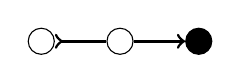
\begin{tikzpicture}[%
  wnode/.style={circle,fill=white,draw},
  bnode/.style={circle,fill=black,draw},
  thickline/.style={line width=1pt}]
  \node[wnode] (O) {};
  \node[wnode] (O1) [left of=O]  {};
  \node[bnode] (N1) [right of=O] {};
  \path[thickline, >-] (O1) edge (O);
  \draw[thickline,->] (O) to node {} (N1);
\end{tikzpicture}

  }
  \subfloat[][$\mathcal{S}^2$]{
    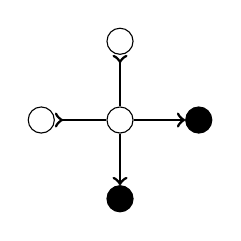
\begin{tikzpicture}[%
  wnode/.style={circle,fill=white,draw},
  bnode/.style={circle,fill=black,draw},
  thickline/.style={line width=1pt}]
  \node[wnode] (O) {};
  \node[wnode] (O1) [left of=O]  {};
  \node[wnode] (O2) [above of=O]  {};
  \node[bnode] (N1) [right of=O] {};
  \node[bnode] (N2) [below of=O] {};
  \path[thickline, >-] (O1) edge (O);
  \path[thickline, >-] (O2) edge (O);
  \draw[thickline,->] (O) to node {} (N1);
  \draw[thickline,->] (O) to node {} (N2);
\end{tikzpicture}

  }
  \subfloat[][$\mathcal{S}^3$]{
    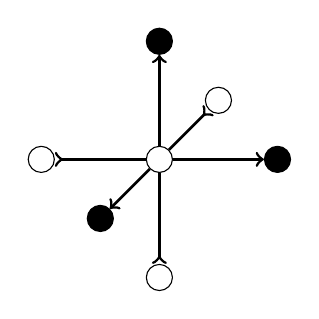
\begin{tikzpicture}[%
  node distance=1.5cm, auto,
  wnode/.style={circle,fill=white,draw},
  bnode/.style={circle,fill=black,draw},
  thickline/.style={line width=1pt}]
  \node[wnode] (O) {};
  \node[wnode] [left of=O] (O1) {};
  \node[wnode] [right of=O, above of=O, node distance=0.75cm] (O2) {};
  \node[wnode] [below of=O] (O3) {};
  \node[bnode] (N1) [right of=O] {};
  \node[bnode] (N2) [left of=O, below of=O, node distance=0.75cm] {};
  \node[bnode] (N3) [above of=O] {};
  \path[thickline, >-] (O1) edge (O);
  \path[thickline, >-] (O2) edge (O);
  \path[thickline, >-] (O3) edge (O);
  \draw[thickline,->] (O) to node {} (N1);
  \draw[thickline,->] (O) to node {} (N2);
  \draw[thickline,->] (O) to node {} (N3);
\end{tikzpicture}

  } \\
    \caption[Full recursion stencils in one, two and three dimensions]{The basis
    function recursion stencils in one, two and three dimensions. The black nodes
    can be computed given the white ones. This works in one single step, i.e.
    we need all white ones and get all black ones.}
    \label{fig:recursion_stencils_full}
\end{figure}

For all these recurrences we need starting points. The only point we know is $\phi_{\vec{0}}$.
But as we found earlier we can insert a $0$ for all $\vec{k}$ where $\exists k_d$ with $k_d < 0$.
Hence we have indeed enough known values to get the process started. An example
of how this works in two dimensions is shown in figure \ref{fig:naive_stencil_application}
and algorithm \ref{al:eval_phik_DD_naive}.

\begin{figure}
  \centering
  \begin{tikzpicture}[%
    func/.style={scale=0.8,color=gray},
    zero/.style={scale=0.8,color=black}]

    \node[zero] (v0m1) at (1,0) {$0$};
    \node[zero] (v1m1) at (2,0) {$0$};
    \node[zero] (v2m1) at (3,0) {$0$};
    \node[zero] (v3m1) at (4,0) {$0$};

    \node[zero] (vm10) at (0,1) {$0$};
    \node[zero] (vm11) at (0,2) {$0$};
    \node[zero] (vm12) at (0,3) {$0$};
    \node[zero] (vm13) at (0,4) {$0$};

    \node[func,color=black] (v00) at (1,1) {$\phi_{0,0}$};

    \node[func,color=blue] (v01) at (1,2) {$\phi_{0,1}$};
    \node[func,color=green] (v02) at (1,3) {$\phi_{0,2}$};
    \node[func] (v03) at (1,4) {$\phi_{0,3}$};

    \node[func,color=blue] (v10) at (2,1) {$\phi_{1,0}$};
    \node[func,color=green] (v11) at (2,2) {$\phi_{1,1}$};
    \node[func] (v12) at (2,3) {$\phi_{1,2}$};
    \node[func] (v13) at (2,4) {$\phi_{1,3}$};

    \node[func,color=green] (v20) at (3,1) {$\phi_{2,0}$};
    \node[func] (v21) at (3,2) {$\phi_{2,1}$};
    \node[func] (v22) at (3,3) {$\phi_{2,2}$};
    \node[func] (v23) at (3,4) {$\phi_{2,3}$};

    \node[func] (v30) at (4,1) {$\phi_{3,0}$};
    \node[func] (v31) at (4,2) {$\phi_{3,1}$};
    \node[func] (v32) at (4,3) {$\phi_{3,2}$};
    \node[func] (v33) at (4,4) {$\phi_{3,3}$};

    \begin{scope}
    \draw[draw=green!80,line width=0.8pt] ($(v10)+(0.0,0.3)$)
        to[out=190,in=350] ($(v00)+(0.0,0.3)$)
        to[out=170,in=90] ($(v00)+(-0.3,0.0)$)
        to[out=270,in=190] ($(v00)+(0.0,-0.3)$)
        to[out=10,in=80] ($(v1m1)+(-0.2,0.0)$)
        to[out=260,in=180] ($(v1m1)+(0.0,-0.2)$)
        to[out=0,in=280] ($(v1m1)+(0.2,0.0)$)
        to[out=100,in=260] ($(v10)+(0.3,0.0)$)
        to[out=80,in=10] ($(v10)+(0.0,0.3)$);
    \draw[draw=green!80,->,line width=0.8pt] ($(v10)+(0.0,0.3)$) -- (v11);
    \draw[draw=green!80,->,line width=0.8pt] ($(v10)+(0.3,0.0)$) -- (v20);
    \end{scope}

    \begin{scope}
    \draw[draw=green!80,line width=0.8pt] ($(v01)+(0.0,0.3)$)
        to[out=190,in=350] ($(vm11)+(0.0,0.2)$)
        to[out=170,in=90] ($(vm11)+(-0.2,0.0)$)
        to[out=270,in=190] ($(vm11)+(0.0,-0.2)$)
        to[out=10,in=80] ($(v00)+(-0.3,0.0)$)
        to[out=260,in=180] ($(v00)+(0.0,-0.3)$)
        to[out=0,in=280] ($(v00)+(0.3,0.0)$)
        to[out=100,in=260] ($(v01)+(0.3,0.0)$)
        to[out=80,in=10] ($(v01)+(0.0,0.3)$);
    \draw[draw=green!80,->,line width=0.8pt] ($(v01)+(0.0,0.3)$) -- (v02);
    \draw[draw=green!80,->,line width=0.8pt] ($(v01)+(0.3,0.0)$) -- (v11);
    \end{scope}

    \begin{scope}
    \draw[draw=blue!100,line width=0.8pt] ($(v00)+(0.0,0.3)$)
        to[out=190,in=350] ($(vm10)+(0.0,0.2)$)
        to[out=170,in=90] ($(vm10)+(-0.2,0.0)$)
        to[out=270,in=190] ($(vm10)+(0.0,-0.2)$)
        to[out=10,in=80] ($(v0m1)+(-0.2,0.0)$)
        to[out=260,in=180] ($(v0m1)+(0.0,-0.2)$)
        to[out=0,in=280] ($(v0m1)+(0.2,0.0)$)
        to[out=100,in=260] ($(v00)+(0.3,0.0)$)
        to[out=80,in=10] ($(v00)+(0.0,0.3)$);
    \draw[draw=blue,->,line width=0.8pt] ($(v00)+(0.0,0.3)$) -- (v01);
    \draw[draw=blue,->,line width=0.8pt] ($(v00)+(0.3,0.0)$) -- (v10);
    \end{scope}
\end{tikzpicture}

  \caption[Naive stencil application in two dimensions]{Naive stencil application
           in two dimensions. All values we initially know are printed in black.
           In a first step we centre the stencil $\mathcal{S}^2$ at the node
           $\vec{k} = (0,0)$ (blue) and compute $\phi_{0,1}$ and $\phi_{1,0}$.
           Next we can apply the stencil there (green) and find $\phi_{0,2}$,
           $\phi_{1,1}$ and $\phi_{2,0}$.}
  \label{fig:naive_stencil_application}
\end{figure}

\begin{algorithm}
  \caption{Evaluate higher order states $\phi_k$ recursively (naive version)}
  \label{al:eval_phik_DD_naive}
  \begin{algorithmic}
    \REQUIRE The number $D$ of space dimensions
    \REQUIRE The Hagedorn parameter set $\Pi = \{q,p,Q,P\}$
    \REQUIRE The semi-classical scaling parameter $\varepsilon$
    \REQUIRE The basis shape $\mathfrak{K}$ and its linearisation mapping $\mu$
    \REQUIRE The grid node $\vec{\gamma} \in \mathbb{R}^D$

    \STATE // Storage space for the result
    \STATE $\vec{\psi} \assign \vec{0} \in \mathbb{C}^{|\mathfrak{K}|}$

    \STATE // Evaluate the ground state by algorithm \ref{al:eval_phi0_DD}
    \STATE $\vec{\psi}[\mu(\vec{0})] = \text{\bf{evaluate\_ground\_state}}(D, \Pi, \varepsilon, \vec{\gamma})$

    \STATE // Loop over the multi-indices
    \FOR{$\vec{k} \in \mathfrak{K}$}
      \STATE // Backward neighbours
      \STATE $\vec{\xi} \assign \vec{0} \in \mathbb{C}^{D}$
      \FOR{$d = 0$ \TO $d = D-1$}
        \STATE $\vec{k}^\prime \assign \vec{k} - \vec{e}^{d}$
        \IF{$\vec{k}^\prime \in \mathfrak{K}$}
          \STATE $\vec{\xi}[d] = \sqrt{\vec{k}[d]} \, \vec{\psi}[\mu(\vec{k}^\prime)]$
        \ENDIF
      \ENDFOR

      \STATE // Compute 3-term recursion
      \STATE $\vec{\alpha} \assign (\vec{\gamma} - \vec{q}) \, \vec{\psi}[\mu(\vec{k})]$
      \STATE $\vec{\beta_1} \assign \sqrt{\frac{2}{\varepsilon^2}} \, \mat{Q}\inv \cdot \vec{\alpha}$
      \STATE $\vec{\beta_2} \assign \mat{Q}\inv \conj{\mat{Q}} \cdot \vec{\xi}$
      \STATE $\vec{\beta} \assign \vec{\beta_1} - \vec{\beta_2}$

      \STATE // Store the results at the correct positions (forward neighbours)
      \FOR{$d = 0$ \TO $d = D-1$}
        \STATE $\vec{k}^\prime \assign \vec{k} + \vec{e}^d$
        \IF{$\vec{k}^\prime \in \mathfrak{K}$}
          \STATE $\vec{\psi}[\mu(\vec{k}^\prime)] = \frac{\vec{\beta}[d]}{\sqrt{\vec{k}[d] + 1}}$
        \ENDIF
      \ENDFOR
  \ENDFOR

  \STATE // Whether to include the problematic prefactor or not
  \STATE // Make sure not to divide twice for $\phi_{\vec{0}}$!
  \IF{prefactor is True}
    \STATE $\vec{\psi} = \frac{1}{\sqrt{\det\mat{Q}}} \, \vec{\psi}$
  \ENDIF

  \RETURN $\vec{\psi}$
\end{algorithmic}
\end{algorithm}

The most severe issue with this naive stencil application is that we compute almost
all functions twice, here this becomes obvious the first time for $\phi_{1,1}$.
Even worse, in $D$ dimensions we would compute almost all functions $D$ times!

Therefore we seek a better way to organise the computations. To achieve this goal we
modify the stencil in a way that seems to be counter intuitive at first. Define the
modified \emph{cheap stencil} as follows.

\begin{definition}[Cheap recursion stencil]
  The cheap recursion stencil does not compute all $D$ outputs $\phi_{\vec{k}+\vec{e}^d}$
  for all $d \in [0, \ldots, D-1]$ but only one output for a single and fixed direction $d$.
  We denote the cheap stencil for direction $d$ and in $D$ dimensions by $\mathcal{S}_d^D$.
  In $D$ dimensions we have $D$ different stencils:
  \begin{equation*}
    \mathcal{S}^D_d \quad d \in [0, \ldots, D-1] \, .
  \end{equation*}
\end{definition}

Figures \ref{fig:recursion_stencils_cheap_2D} and \ref{fig:recursion_stencils_cheap_3D}
give an impression how the stencils look like and how they work in two and three
dimensions. In one dimension we obviously find $\mathcal{S}^1_0 \equiv \mathcal{S}^1$.
In all dimensions it holds that we recover the full stencil $\mathcal{S}^D$ as the sum:

\begin{equation*}
  \mathcal{S}^D = \bigoplus_{d=0}^{D-1} \mathcal{S}^D_d
\end{equation*}

where all stencils are applied centred at the very same node $\phi_{\vec{k}}$.

\begin{figure}[h!]
  \centering
  \subfloat[][$\mathcal{S}^2_0$]{
    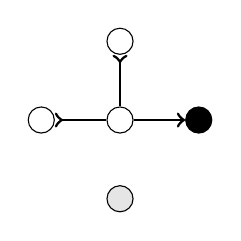
\begin{tikzpicture}[%
  wnode/.style={circle,fill=white,draw},
  bnode/.style={circle,fill=black,draw},
  gnode/.style={circle,fill=black!10,draw},
  thickline/.style={line width=1pt}]
  \node[wnode] (O) {};
  \node[wnode] (O1) [left of=O]  {};
  \node[wnode] (O2) [above of=O]  {};
  \node[bnode] (N1) [right of=O] {};
  \node[gnode] (N2) [below of=O] {};
  \path[thickline, >-] (O1) edge (O);
  \path[thickline, >-] (O2) edge (O);
  \draw[thickline,->] (O) to node {} (N1);
\end{tikzpicture}

  }
  \subfloat[][$\mathcal{S}^2_1$]{
    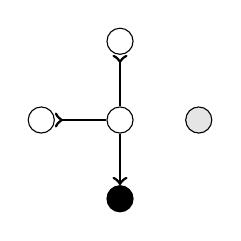
\begin{tikzpicture}[%
  wnode/.style={circle,fill=white,draw},
  bnode/.style={circle,fill=black,draw},
  gnode/.style={circle,fill=black!10,draw},
  thickline/.style={line width=1pt}]
  \node[wnode] (O) {};
  \node[wnode] (O1) [left of=O]  {};
  \node[wnode] (O2) [above of=O]  {};
  \node[gnode] (N1) [right of=O] {};
  \node[bnode] (N2) [below of=O] {};
  \path[thickline, >-] (O1) edge (O);
  \path[thickline, >-] (O2) edge (O);
  \draw[thickline,->] (O) to node {} (N2);
\end{tikzpicture}

  } \\
    \caption[Cheap recursion stencils in two dimensions]{The modified basis
    function recursion stencils $\mathcal{S}^2_d$ in two dimensions.
    The black node can be computed given the white nodes. The grey node would be
    computed by the full stencil $\mathcal{S}^2$ but is intentionally left out by
    the modified ones.}
    \label{fig:recursion_stencils_cheap_2D}
\end{figure}

\begin{figure}[h!]
  \centering
  \subfloat[][$\mathcal{S}^3_0$]{
    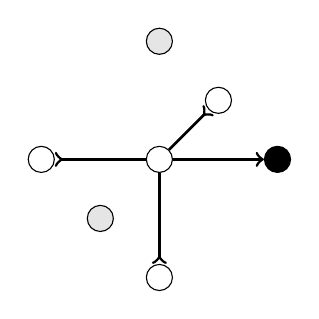
\begin{tikzpicture}[%
  node distance=1.5cm, auto,
  wnode/.style={circle,fill=white,draw},
  bnode/.style={circle,fill=black,draw},
  gnode/.style={circle,fill=black!10,draw},
  thickline/.style={line width=1pt}]
  \node[wnode] (O) {};
  \node[wnode] [left of=O] (O1) {};
  \node[wnode] [right of=O, above of=O, node distance=0.75cm] (O2) {};
  \node[wnode] [below of=O] (O3) {};
  \node[bnode] (N1) [right of=O] {};
  \node[gnode] (N2) [left of=O, below of=O, node distance=0.75cm] {};
  \node[gnode] (N3) [above of=O] {};
  \path[thickline, >-] (O1) edge (O);
  \path[thickline, >-] (O2) edge (O);
  \path[thickline, >-] (O3) edge (O);
  \draw[thickline,->] (O) to node {} (N1);
\end{tikzpicture}

  }
  \subfloat[][$\mathcal{S}^3_1$]{
    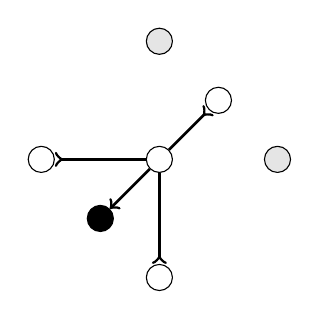
\begin{tikzpicture}[%
  node distance=1.5cm, auto,
  wnode/.style={circle,fill=white,draw},
  bnode/.style={circle,fill=black,draw},
  gnode/.style={circle,fill=black!10,draw},
  thickline/.style={line width=1pt}]
  \node[wnode] (O) {};
  \node[wnode] [left of=O] (O1) {};
  \node[wnode] [right of=O, above of=O, node distance=0.75cm] (O2) {};
  \node[wnode] [below of=O] (O3) {};
  \node[gnode] (N1) [right of=O] {};
  \node[bnode] (N2) [left of=O, below of=O, node distance=0.75cm] {};
  \node[gnode] (N3) [above of=O] {};
  \path[thickline, >-] (O1) edge (O);
  \path[thickline, >-] (O2) edge (O);
  \path[thickline, >-] (O3) edge (O);
  \draw[thickline,->] (O) to node {} (N2);
\end{tikzpicture}

  }
  \subfloat[][$\mathcal{S}^3_2$]{
    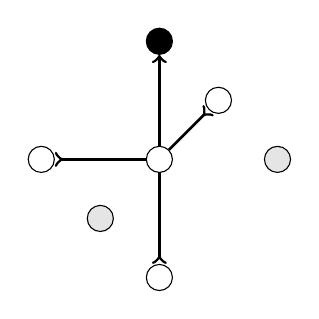
\begin{tikzpicture}[%
  node distance=1.5cm, auto,
  wnode/.style={circle,fill=white,draw},
  bnode/.style={circle,fill=black,draw},
  gnode/.style={circle,fill=black!10,draw},
  thickline/.style={line width=1pt}]
  \node[wnode] (O) {};
  \node[wnode] [left of=O] (O1) {};
  \node[wnode] [right of=O, above of=O, node distance=0.75cm] (O2) {};
  \node[wnode] [below of=O] (O3) {};
  \node[gnode] (N1) [right of=O] {};
  \node[gnode] (N2) [left of=O, below of=O, node distance=0.75cm] {};
  \node[bnode] (N3) [above of=O] {};
  \path[thickline, >-] (O1) edge (O);
  \path[thickline, >-] (O2) edge (O);
  \path[thickline, >-] (O3) edge (O);
  \draw[thickline,->] (O) to node {} (N3);
\end{tikzpicture}

  } \\
    \caption[Cheap recursion stencils in three dimensions]{The modified basis
    function recursion stencils $\mathcal{S}^3_d$ in three dimensions.
    The black node can be computed given the white nodes. The grey nodes would be
    computed by the full stencil $\mathcal{S}^3$ but is intentionally left out by
    the modified ones.}
    \label{fig:recursion_stencils_cheap_3D}
\end{figure}

Formally we have just used the $d$-th row of equation \eqref{eq:basis_recursion_DD} only
to compute the application of $\mathcal{S}^D_d$ to $\phi_{\vec{k}}$. By using colon or
slicing notation we can write the formula for the modified stencils $\mathcal{S}^D_d$
as follows:

\begin{equation}
  \sqrt{k_d +1} \phi_{k + e_d}
  = \sqrt{\frac{2}{\varepsilon^2}}
  \left(Q^{-1}\right)_{d,:}
  \left( x-q \right)
  \phi_{k}
  -
  \left(Q^{-1} \overline{Q} \right)_{d,:}
  \begin{pmatrix}
    \sqrt{k_0} \phi_{k - e_0} \\
    \vdots \\
    \sqrt{k_{D-1}} \phi_{k - e_{D-1}}
  \end{pmatrix} \,.
\end{equation}

What can we do with these modified stencils? And why should they be more efficient?
The most important gain is that we do never compute any function twice. But for this
we have to use the new stencils in a clever way. We start with an empty grid like the
one in figure \ref{fig:naive_stencil_application}. It contains only the ground state
evaluated $\phi_{\vec{0}}$. Now we apply the stencil $\mathcal{S}^D_0$ along the first
direction $d=0$ until we overflow. This works fine as we use the ground state as
anchor point for this \emph{recursion chain} and produce new anchor points successively.
This process is shown in figure \ref{fig:efficient_stencil_application_d0}.

\begin{figure}
  \centering
  \begin{tikzpicture}[%
    func/.style={scale=0.8,color=gray},
    zero/.style={scale=0.8,color=black}]

    \node[zero] (v0m1) at (1,0) {$0$};
    \node[zero] (v1m1) at (2,0) {$0$};
    \node[zero] (v2m1) at (3,0) {$0$};
    \node[zero] (v3m1) at (4,0) {$0$};

    \node[zero] (vm10) at (0,1) {$0$};
    \node[zero] (vm11) at (0,2) {$0$};
    \node[zero] (vm12) at (0,3) {$0$};
    \node[zero] (vm13) at (0,4) {$0$};

    \node[func,color=black] (v00) at (1,1) {$\phi_{0,0}$};

    \node[func] (v01) at (1,2) {$\phi_{0,1}$};
    \node[func] (v02) at (1,3) {$\phi_{0,2}$};
    \node[func] (v03) at (1,4) {$\phi_{0,3}$};

    \node[func,color=blue] (v10) at (2,1) {$\phi_{1,0}$};
    \node[func] (v11) at (2,2) {$\phi_{1,1}$};
    \node[func] (v12) at (2,3) {$\phi_{1,2}$};
    \node[func] (v13) at (2,4) {$\phi_{1,3}$};

    \node[func,color=blue] (v20) at (3,1) {$\phi_{2,0}$};
    \node[func] (v21) at (3,2) {$\phi_{2,1}$};
    \node[func] (v22) at (3,3) {$\phi_{2,2}$};
    \node[func] (v23) at (3,4) {$\phi_{2,3}$};

    \node[func,color=blue] (v30) at (4,1) {$\phi_{3,0}$};
    \node[func] (v31) at (4,2) {$\phi_{3,1}$};
    \node[func] (v32) at (4,3) {$\phi_{3,2}$};
    \node[func] (v33) at (4,4) {$\phi_{3,3}$};

    \begin{scope}
    \draw[draw=blue!60,line width=0.8pt] ($(v20)+(0.0,0.3)$)
        to[out=190,in=350] ($(v10)+(0.0,0.3)$)
        to[out=170,in=90] ($(v10)+(-0.3,0.0)$)
        to[out=270,in=190] ($(v10)+(0.0,-0.3)$)
        to[out=10,in=80] ($(v2m1)+(-0.2,0.0)$)
        to[out=260,in=180] ($(v2m1)+(0.0,-0.2)$)
        to[out=0,in=280] ($(v2m1)+(0.2,0.0)$)
        to[out=100,in=260] ($(v20)+(0.3,0.0)$)
        to[out=80,in=10] ($(v20)+(0.0,0.3)$);
    \draw[draw=blue!60,->,line width=0.8pt] ($(v20)+(0.3,0.0)$) -- (v30);
    \end{scope}

    \begin{scope}
    \draw[draw=blue!80,line width=0.8pt] ($(v10)+(0.0,0.3)$)
        to[out=190,in=350] ($(v00)+(0.0,0.3)$)
        to[out=170,in=90] ($(v00)+(-0.3,0.0)$)
        to[out=270,in=190] ($(v00)+(0.0,-0.3)$)
        to[out=10,in=80] ($(v1m1)+(-0.2,0.0)$)
        to[out=260,in=180] ($(v1m1)+(0.0,-0.2)$)
        to[out=0,in=280] ($(v1m1)+(0.2,0.0)$)
        to[out=100,in=260] ($(v10)+(0.3,0.0)$)
        to[out=80,in=10] ($(v10)+(0.0,0.3)$);
    \draw[draw=blue!80,->,line width=0.8pt] ($(v10)+(0.3,0.0)$) -- (v20);
    \end{scope}

    \begin{scope}
    \draw[draw=blue!100,line width=0.8pt] ($(v00)+(0.0,0.3)$)
        to[out=190,in=350] ($(vm10)+(0.0,0.2)$)
        to[out=170,in=90] ($(vm10)+(-0.2,0.0)$)
        to[out=270,in=190] ($(vm10)+(0.0,-0.2)$)
        to[out=10,in=80] ($(v0m1)+(-0.2,0.0)$)
        to[out=260,in=180] ($(v0m1)+(0.0,-0.2)$)
        to[out=0,in=280] ($(v0m1)+(0.2,0.0)$)
        to[out=100,in=260] ($(v00)+(0.3,0.0)$)
        to[out=80,in=10] ($(v00)+(0.0,0.3)$);
    \draw[draw=blue,->,line width=0.8pt] ($(v00)+(0.3,0.0)$) -- (v10);
    \end{scope}
\end{tikzpicture}

  \caption[Efficient stencil application in two dimensions]{
           First step in the efficient application of the recursion stencils
           in two dimensions. All values we initially know are printed in black.
           In a first step we centre the cheap stencil $\mathcal{S}^2_0$ at the
           node $\vec{k} = (0,0)$ and compute $\phi_{1,0}$ only. Next we can use
           the same stencil centred at $\phi_{1,0}$ and find $\phi_{2,0}$. We
           continue like this until an overflow occurs. (In this little example
           we are done after the next step.)}
  \label{fig:efficient_stencil_application_d0}
\end{figure}

After this first step we can not apply the stencil $\mathcal{S}^2_0$ anymore.
There is no anchor point left that would give us new nodes in the lattice.
But we have build a whole chain $\phi_{k, 0}$ of starting points. Hence we take
the stencil $\mathcal{S}^2_1$ at hand and go along the second direction $d=1$
starting a chain for each $\phi_{k,0}$. Again we follow each chain until an
overflow occurs. Note that we must do this in increasing order of the index $k$
because we need the values to the left of where we centre $\mathcal{S}^2_1$.
Figure \ref{fig:efficient_stencil_application_d1} shows the process for the
first two chains starting at $\phi_{0,0}$ and $\phi_{1,0}$.

\begin{figure}[h!]
  \centering
  \subfloat[][]{
    \begin{tikzpicture}[%
    func/.style={scale=0.8,color=gray},
    zero/.style={scale=0.8,color=black}]

    \node[zero] (v0m1) at (1,0) {$0$};
    \node[zero] (v1m1) at (2,0) {$0$};
    \node[zero] (v2m1) at (3,0) {$0$};
    \node[zero] (v3m1) at (4,0) {$0$};

    \node[zero] (vm10) at (0,1) {$0$};
    \node[zero] (vm11) at (0,2) {$0$};
    \node[zero] (vm12) at (0,3) {$0$};
    \node[zero] (vm13) at (0,4) {$0$};

    \node[func,color=black] (v00) at (1,1) {$\phi_{0,0}$};

    \node[func,color=green] (v01) at (1,2) {$\phi_{0,1}$};
    \node[func,color=green] (v02) at (1,3) {$\phi_{0,2}$};
    \node[func,color=green] (v03) at (1,4) {$\phi_{0,3}$};

    \node[func,color=black] (v10) at (2,1) {$\phi_{1,0}$};
    \node[func] (v11) at (2,2) {$\phi_{1,1}$};
    \node[func] (v12) at (2,3) {$\phi_{1,2}$};
    \node[func] (v13) at (2,4) {$\phi_{1,3}$};

    \node[func,color=black] (v20) at (3,1) {$\phi_{2,0}$};
    \node[func] (v21) at (3,2) {$\phi_{2,1}$};
    \node[func] (v22) at (3,3) {$\phi_{2,2}$};
    \node[func] (v23) at (3,4) {$\phi_{2,3}$};

    \node[func,color=black] (v30) at (4,1) {$\phi_{3,0}$};
    \node[func] (v31) at (4,2) {$\phi_{3,1}$};
    \node[func] (v32) at (4,3) {$\phi_{3,2}$};
    \node[func] (v33) at (4,4) {$\phi_{3,3}$};

    \begin{scope}
    \draw[draw=green!60,line width=0.8pt] ($(v02)+(0.0,0.3)$)
        to[out=190,in=350] ($(vm12)+(0.0,0.2)$)
        to[out=170,in=90] ($(vm12)+(-0.2,0.0)$)
        to[out=270,in=190] ($(vm12)+(0.0,-0.2)$)
        to[out=10,in=80] ($(v01)+(-0.3,0.0)$)
        to[out=260,in=180] ($(v01)+(0.0,-0.3)$)
        to[out=0,in=280] ($(v01)+(0.3,0.0)$)
        to[out=100,in=260] ($(v02)+(0.3,0.0)$)
        to[out=80,in=10] ($(v02)+(0.0,0.3)$);
    \draw[draw=green!60,->,line width=0.8pt] ($(v02)+(0.0,0.3)$) -- (v03);
    \end{scope}

    \begin{scope}
    \draw[draw=green!80,line width=0.8pt] ($(v01)+(0.0,0.3)$)
        to[out=190,in=350] ($(vm11)+(0.0,0.2)$)
        to[out=170,in=90] ($(vm11)+(-0.2,0.0)$)
        to[out=270,in=190] ($(vm11)+(0.0,-0.2)$)
        to[out=10,in=80] ($(v00)+(-0.3,0.0)$)
        to[out=260,in=180] ($(v00)+(0.0,-0.3)$)
        to[out=0,in=280] ($(v00)+(0.3,0.0)$)
        to[out=100,in=260] ($(v01)+(0.3,0.0)$)
        to[out=80,in=10] ($(v01)+(0.0,0.3)$);
    \draw[draw=green!80,->,line width=0.8pt] ($(v01)+(0.0,0.3)$) -- (v02);
    \end{scope}

    \begin{scope}
    \draw[draw=green!100,line width=0.8pt] ($(v00)+(0.0,0.3)$)
        to[out=190,in=350] ($(vm10)+(0.0,0.2)$)
        to[out=170,in=90] ($(vm10)+(-0.2,0.0)$)
        to[out=270,in=190] ($(vm10)+(0.0,-0.2)$)
        to[out=10,in=80] ($(v0m1)+(-0.2,0.0)$)
        to[out=260,in=180] ($(v0m1)+(0.0,-0.2)$)
        to[out=0,in=280] ($(v0m1)+(0.2,0.0)$)
        to[out=100,in=260] ($(v00)+(0.3,0.0)$)
        to[out=80,in=10] ($(v00)+(0.0,0.3)$);
    \draw[draw=green,->,line width=0.8pt] ($(v00)+(0.0,0.3)$) -- (v01);
    \end{scope}
\end{tikzpicture}

  }
  \hspace{1cm}
  \subfloat[][]{
    \begin{tikzpicture}[%
    func/.style={scale=0.8,color=gray},
    zero/.style={scale=0.8,color=black}]

    \node[zero] (v0m1) at (1,0) {$0$};
    \node[zero] (v1m1) at (2,0) {$0$};
    \node[zero] (v2m1) at (3,0) {$0$};
    \node[zero] (v3m1) at (4,0) {$0$};

    \node[zero] (vm10) at (0,1) {$0$};
    \node[zero] (vm11) at (0,2) {$0$};
    \node[zero] (vm12) at (0,3) {$0$};
    \node[zero] (vm13) at (0,4) {$0$};

    \node[func,color=black] (v00) at (1,1) {$\phi_{0,0}$};

    \node[func,color=black] (v01) at (1,2) {$\phi_{0,1}$};
    \node[func,color=black] (v02) at (1,3) {$\phi_{0,2}$};
    \node[func,color=black] (v03) at (1,4) {$\phi_{0,3}$};

    \node[func,color=black] (v10) at (2,1) {$\phi_{1,0}$};
    \node[func,color=green] (v11) at (2,2) {$\phi_{1,1}$};
    \node[func,color=green] (v12) at (2,3) {$\phi_{1,2}$};
    \node[func,color=green] (v13) at (2,4) {$\phi_{1,3}$};

    \node[func,color=black] (v20) at (3,1) {$\phi_{2,0}$};
    \node[func] (v21) at (3,2) {$\phi_{2,1}$};
    \node[func] (v22) at (3,3) {$\phi_{2,2}$};
    \node[func] (v23) at (3,4) {$\phi_{2,3}$};

    \node[func,color=black] (v30) at (4,1) {$\phi_{3,0}$};
    \node[func] (v31) at (4,2) {$\phi_{3,1}$};
    \node[func] (v32) at (4,3) {$\phi_{3,2}$};
    \node[func] (v33) at (4,4) {$\phi_{3,3}$};

    \begin{scope}
    \draw[draw=green!60,line width=0.8pt] ($(v12)+(0.0,0.3)$)
        to[out=190,in=350] ($(v02)+(0.0,0.3)$)
        to[out=170,in=90] ($(v02)+(-0.3,0.0)$)
        to[out=270,in=190] ($(v02)+(0.0,-0.3)$)
        to[out=10,in=80] ($(v11)+(-0.3,0.0)$)
        to[out=260,in=180] ($(v11)+(0.0,-0.3)$)
        to[out=0,in=280] ($(v11)+(0.3,0.0)$)
        to[out=100,in=260] ($(v12)+(0.3,0.0)$)
        to[out=80,in=10] ($(v12)+(0.0,0.3)$);
    \draw[draw=green!60,->,line width=0.8pt] ($(v12)+(0.0,0.3)$) -- (v13);
    \end{scope}

    \begin{scope}
    \draw[draw=green!80,line width=0.8pt] ($(v11)+(0.0,0.3)$)
        to[out=190,in=350] ($(v01)+(0.0,0.3)$)
        to[out=170,in=90] ($(v01)+(-0.3,0.0)$)
        to[out=270,in=190] ($(v01)+(0.0,-0.3)$)
        to[out=10,in=80] ($(v10)+(-0.3,0.0)$)
        to[out=260,in=180] ($(v10)+(0.0,-0.3)$)
        to[out=0,in=280] ($(v10)+(0.3,0.0)$)
        to[out=100,in=260] ($(v11)+(0.3,0.0)$)
        to[out=80,in=10] ($(v11)+(0.0,0.3)$);
    \draw[draw=green!80,->,line width=0.8pt] ($(v11)+(0.0,0.3)$) -- (v12);
    \end{scope}

    \begin{scope}
    \draw[draw=green!100,line width=0.8pt] ($(v10)+(0.0,0.3)$)
        to[out=190,in=350] ($(v00)+(0.0,0.3)$)
        to[out=170,in=90] ($(v00)+(-0.3,0.0)$)
        to[out=270,in=190] ($(v00)+(0.0,-0.3)$)
        to[out=10,in=80] ($(v1m1)+(-0.2,0.0)$)
        to[out=260,in=180] ($(v1m1)+(0.0,-0.2)$)
        to[out=0,in=280] ($(v1m1)+(0.2,0.0)$)
        to[out=100,in=260] ($(v10)+(0.3,0.0)$)
        to[out=80,in=10] ($(v10)+(0.0,0.3)$);
    \draw[draw=green,->,line width=0.8pt] ($(v10)+(0.0,0.3)$) -- (v11);
    \end{scope}

\end{tikzpicture}

  }
 \\
  \caption[Efficient stencil application in two dimensions]{
           Second step in the efficient application of the recursion stencils
           in two dimensions. All values we initially know are printed in black.
           In a first step we centre the cheap stencil $\mathcal{S}^2_1$ at the
           node $\vec{k} = (0,0)$ and compute $\phi_{0,1}$ only. Next we can use
           the same stencil centred at $\phi_{0,1}$ and find $\phi_{0,2}$. We
           continue like this until an overflow occurs. (In this little example
           we are done after the next step.) Now we can start the second chain
           at the anchor $(1,0)$ and recursively compute $\phi_{1,1}$, $\phi_{1,2}$,
           $\phi_{1,3}$ until the overflow occurs. In a next step (not shown here)
           we start a chain at $(2,0)$, then at $(3,0)$ and so forth until
           the last node $(k,0)$.}
    \label{fig:efficient_stencil_application_d1}
\end{figure}

For a three-index recursion evaluating all the functions $\phi_{k_0,k_1,k_2}$
we would start with a chain along the first dimension computing all $\phi_{k_0, 0, 0}$.
Then we build new chains along the second direction starting one at each of the nodes
$\phi_{k_0, 0, 0}$ and computing all $\phi_{k_0, k_1, 0}$. And finally we build
chains starting at the functions $\phi_{k_0, k_1, 0}$ which gives us all the remaining
functions $\phi_{k_0, k_1, k_2}$.
If we do this correctly we never compute any function more than once and nonetheless
get all functions evaluated. Since we are building chains starting at some node $\vec{k}$
going along a given direction $d$ we call this procedure \emph{chain building}.
And we need a very specialised way of iterating over all $\vec{k} \in \mathfrak{K}$
which we call \emph{chain mode iteration} (compared to, for example, \emph{lexicographical
iteration}).

\begin{definition}[Chain mode basis shape iterator]
  An iterator $\mathcal{I}$ is just a list of multi-indices with a well specified order.
  By iteration over this list we retrieve the contained values in this fixed sequence.
  Given a basis shape $\mathfrak{K}$ in $D$ dimensions we can obtain $D$ different chain
  mode iterators $\mathcal{I}^D_d$ for $d \in [0, \ldots, D-1]$. Any iterator
  is tightly related to the basis shape it belongs to. For that reason we sometimes write
  $\mathcal{I}^D_d[\mathfrak{K}]$ to make this important connection absolutely manifest.
  Clearly the intersection $\mathcal{I}_d \cap \mathcal{I}_{d^\prime}$ is never empty
  since all iterators $\mathcal{I}_d$ contain the multi-index $\vec{0}$ as starting point.
\end{definition}

Referring back to the figures \ref{fig:efficient_stencil_application_d0} and \ref{fig:efficient_stencil_application_d1}
we computed all the $\phi_{\vec{k}}$ for $\vec{k} \in \mathcal{I}^2_0$ and $\vec{k} \in \mathcal{I}^2_1$
respectively. The iterator $\mathcal{I}^2_0$ there yields the values $(0,0)$, $(1,0)$ and $(2,0)$
in this order and then gets exhausted. The next higher iterator $\mathcal{I}^2_1$ gives the values
$(0,0)$, $(0,1)$, $(0,2)$, $(1,0)$, $(1,1)$, $(1,2)$, \ldots, $(3,0)$, $(3,1)$, $(3,2)$ before it
gets exhausted too.

Going back to the general $D$ dimensional case and an arbitrary basis shape $\mathfrak{K}$
we recognise that each iterator $\mathcal{I}^D_d[\mathfrak{K}]$ exactly yields the nodes
$\vec{k} \in \mathfrak{K}$ where we have to apply the modified stencil $\mathcal{S}^D_d$.
This is the quintessence of this whole idea! Now we are ready to formulate the algorithm
\ref{al:eval_phik_DD} for efficient basis evaluation.

\begin{algorithm}
  \caption{Evaluate higher order states $\phi_k$ recursively (efficient version)}
  \label{al:eval_phik_DD}
  \begin{algorithmic}
    \REQUIRE The number $D$ of space dimensions
    \REQUIRE The Hagedorn parameter set $\Pi = \{q,p,Q,P\}$
    \REQUIRE The semi-classical scaling parameter $\varepsilon$
    \REQUIRE The basis shape $\mathfrak{K}$ and its linearisation mapping $\mu$
    \REQUIRE The grid node $\vec{\gamma} \in \mathbb{R}^D$

    \STATE // Storage space for the result
    \STATE $\vec{\psi} \assign \vec{0} \in \mathbb{C}^{|\mathfrak{K}|}$

    \STATE // Evaluate the ground state by algorithm \ref{al:eval_phi0_DD}
    \STATE $\vec{\psi}[\mu(\vec{0})] = \text{\bf{evaluate\_ground\_state}}(D, \Pi, \varepsilon, \vec{\gamma})$

    \STATE // Loop over the directions
    \FOR{$d=0$ \TO $d=D-1$}
      \STATE // Get the iterator
      \STATE $\mathcal{I}_d \assign \text{\bf{chain\_mode\_iterator}}(\mathfrak{K}, d)$

      \STATE // Start the chain building process
      \FOR{$\vec{k} \in \mathcal{I}_d$}

        \STATE // Backward neighbours
        \STATE $\vec{\xi} \assign \vec{0} \in \mathbb{C}^{D}$
        \FOR{$d^\prime = 0$ \TO $d^\prime = D-1$}
          \STATE $\vec{k}^\prime \assign \vec{k} - \vec{e}^{d^\prime}$
          \IF{$\vec{k}^\prime \in \mathfrak{K}$}
            \STATE $\vec{\xi}[d^\prime] = \sqrt{\vec{k}[d^\prime]} \, \vec{\psi}[\mu(\vec{k}^\prime)]$
          \ENDIF
        \ENDFOR

        \STATE // Compute 3-term recursion
        \STATE $\vec{\alpha} \assign (\vec{\gamma} - \vec{q}) \, \vec{\psi}[\mu(\vec{k})]$
        \STATE $\beta_1 \assign \sqrt{\frac{2}{\varepsilon^2}} \, (\mat{Q}\inv)[d,:] \cdot \vec{\alpha}$
        \STATE $\beta_2 \assign (\mat{Q}\inv \conj{\mat{Q}})[d,:] \cdot \vec{\xi}$

        \STATE // Store the result in correct position (forward neighbour in direction $d$)
        \STATE $\vec{k}^\prime \assign \vec{k} + \vec{e}^d$

        \IF{$\vec{k}^\prime \in \mathfrak{K}$}
          \STATE $\vec{\psi}[\mu(\vec{k}^\prime)] = \frac{\beta_1 - \beta_2}{\sqrt{\vec{k}[d] + 1}}$
        \ENDIF
      \ENDFOR
    \ENDFOR

  \STATE // Whether to include the problematic prefactor or not
  \STATE // Make sure not to divide twice for $\phi_{\vec{0}}$!
  \IF{prefactor is True}
    \STATE $\vec{\psi} = \frac{1}{\sqrt{\det\mat{Q}}} \, \vec{\psi}$
  \ENDIF

  \RETURN $\vec{\psi}$
\end{algorithmic}
\end{algorithm}


\begin{algorithm}
\caption{Evaluate the whole basis set $\{\phi_k\}_{k \in \mathfrak{K}}$ on a grid $\Gamma$}
\label{al:eval_phi_basis}
\begin{algorithmic}
    \REQUIRE The basis shape $\mathfrak{K}$
    \REQUIRE The grid $\Gamma$ containing the nodes $\vec{\gamma} \in \mathbb{R}^D$
    \STATE // Storage space for the result
    \STATE $\mat{B} \assign \mat{0} \in \mathbb{C}^{|\mathfrak{K}| \times |\Gamma|}$
    \STATE // Evaluate the basis functions $\{\phi_k\}_{k \in \mathfrak{K}}$ for all grid nodes by algorithm \ref{al:eval_phik_DD}
    \STATE // A real implementation of course exploits vectorisation.
    \FOR{$i=0$ \TO $i=|\Gamma|-1$}
      \STATE $\mat{B}[:, i] = \mathbf{evaluate\_higher\_order\_states}(\gamma_i)$
    \ENDFOR
    \RETURN $\mat{B}$
\end{algorithmic}
\end{algorithm}


Note that all algorithms in this section are quite general and do not depend on
the details of the basis shape $\mathfrak{K}$. We only assume that $\mathfrak{K}$
provides us with enough information about itself. We use the size  $|\mathfrak{K}|$
and we have to get an answer for the question if $\vec{k} \in \mathfrak{K}$. We need
the linearisation mapping $\mu_{\mathfrak{K}}$ and we have to be able to obtain
chain mode iterators $\mathcal{I}^D_d$ for $\mathfrak{K}$. Any reasonable basis shape
implements these functions without much trouble.


\subsection{Number of stencil applications}


We want to count how many times we apply the stencils. Assume we work in a hypercubic
basis shape $\mathfrak{K}$ where the limits are given as $K = [K_0, \ldots, K_{D-1}]$.

For the full stencil $\mathcal{S}^D$ this is easy. We have to apply it maximally
$\prod_{d=0}^{D-1} K_d$ times. And a more careful analysis shows that we have to
apply it exactly:

\begin{equation}
  \prod_{d=0}^{D-1} (K_d -1) +1
\end{equation}

times where the last $1$ is to get the node $\phi_{\vec{K}-\vec{1}}$. This is only
necessary for $D > 1$.

For the modified stencils this gets more complicated. The number of applications
of each individual stencil is given in the table below.

\begin{center}
\begin{tabular}{cl}
  Stencil            & Number of applications \\
  \hline \\
  $\mathcal{S}^D_0$ & $K_0-1$ \\
  $\mathcal{S}^D_1$ & $K_0 (K_1-1)$ \\
  $\mathcal{S}^D_2$ & $K_0 K_1 (K_2-1)$ \\
  $\vdots$ & \\
  $\mathcal{S}^D_{d}$ & $\prod_{i=0}^{d-1} K_i (K_d-1)$ \\
  $\vdots$ & \\
  $\mathcal{S}^D_{D-1}$ & $\prod_{i=0}^{D-2} K_i (K_{D-1}-1)$
\end{tabular}
\end{center}

Now the overall number of stencil applications is then:

\begin{align*}
  \sum_{d=0}^{D-1} \prod_{i=0}^{d-1} K_i (K_d-1)
  & = \sum_{d=0}^{D-1} \left((K_d-1) \prod_{i=0}^{d-1} K_i \right)
   = \sum_{d=0}^{D-1} \left( \prod_{i=0}^{d} K_i - \prod_{i=0}^{d-1} K_i \right) \\
  & = \sum_{d=0}^{D-1} \prod_{i=0}^{d} K_i - \sum_{d=0}^{D-1} \prod_{i=0}^{d-1} K_i \\
  & = \prod_{i=0}^{D-1} K_i - \prod_{i=0}^{-1} K_i = \prod_{i=0}^{D-1} K_i -1
\end{align*}

where the sum is resolved via telescoping and we define the empty product
as the multiplicative identity. Of course it holds that:

\begin{equation*}
  \prod_{d=0}^{D-1} (K_d -1) +1 \leq \prod_{d=0}^{D-1} K_d -1
\end{equation*}

for large enough $K$ and $D$. The consequence is that we perform \emph{more}
applications when using the modified stencil. But it will turn out that this
is not a bad fact. An example in 6 dimensions is shown in figure \ref{fig:number_stencil_applications}.

\begin{figure}
  \centering
  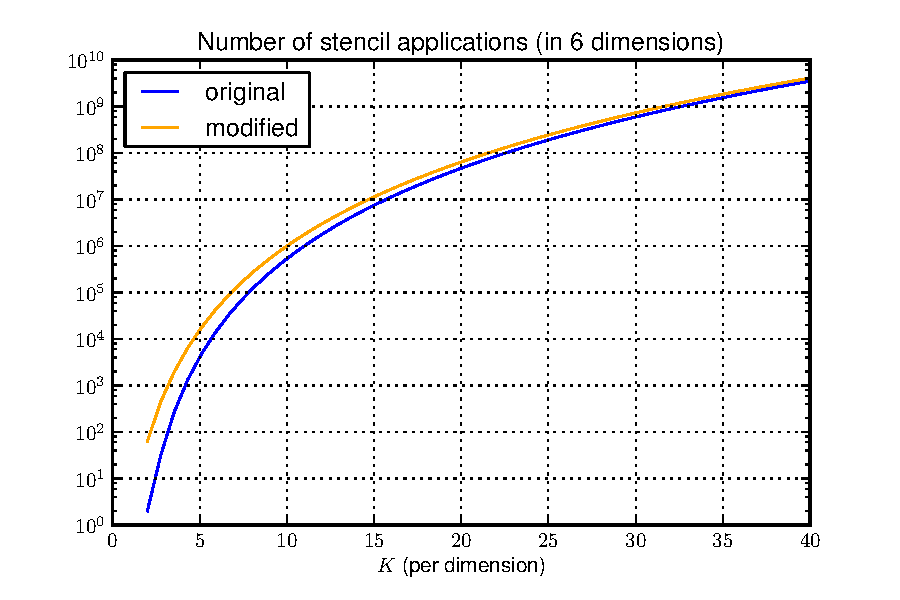
\includegraphics[scale=0.5]{./fig/number_stencil_applications.pdf}
  \caption{Total number of stencil applications for a hypercubic basis shape
           in $D=6$ dimensions and with $K$ nodes along each direction.}
  \label{fig:number_stencil_applications}
\end{figure}


\subsection{Cost of a stencil application}


We define the cost of a stencil application $\mathcal{S} \phi_{\vec{k}}$ as the
number of multiplications which involve a $\phi$. The reason is that we will
evaluate $\phi_{\vec{k}}$ on large grids with many nodes hence $\phi_{\vec{k}}$
is a very long vector.

During the application of the full stencil $\mathcal{S}^D$ we multiply a
$D$ vector by $\phi$ in the first term. In the second one we multiply
a $D \times D$ matrix by a vector of size $D$ containing a (different) $\phi$
in each element. Hence the application $\mathcal{S}^D \phi_k$ has a total cost
of $D^2+D$.

For the modified stencil we only evaluate the first element of the vector equation
and therefore we compute the product of a scalar with $\phi$ and form an inner
product between two vectors of length $D$, one containing a (different) $\phi$
in each element. The application of any modified stencil $\mathcal{S}^D_d$ has
therefore a total cost of $D+1$ which is linear in the number of dimensions.
Figure \ref{fig:cost_stencil_application} shows the cost of both stencils
as a function of dimension $D$.

\begin{figure}
  \centering
  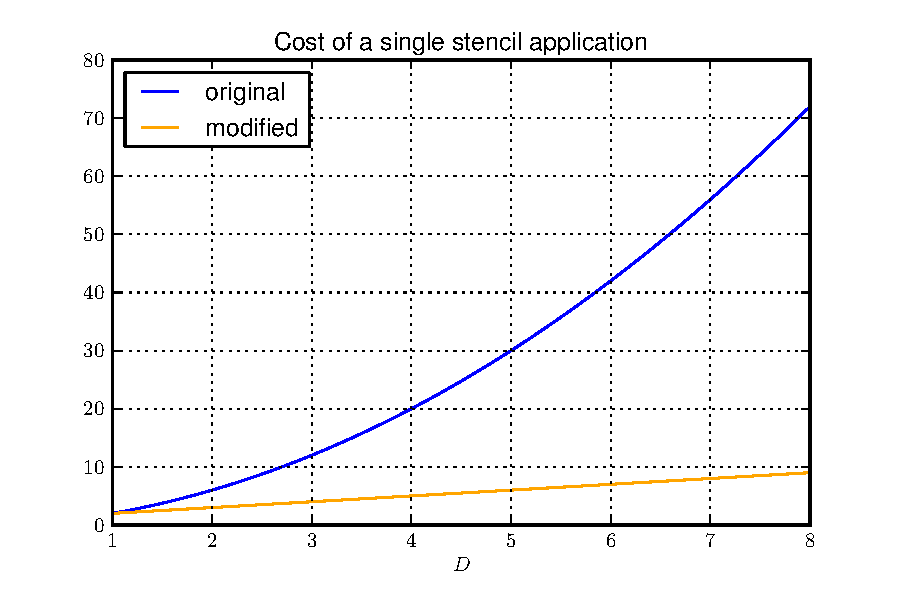
\includegraphics[scale=0.5]{./fig/cost_stencil_application.pdf}
  \caption{The costs of both stencil types in several dimensions.}
  \label{fig:cost_stencil_application}
\end{figure}

If we now compare both evaluation schemes by the number of stencil applications
and the costs of a single application it turns out that the scheme using modified
stencils is much more efficient! In formal notation we find:

\begin{equation*}
  \left(\prod_{d=0}^{D-1} (K_d -1) +1\right) (D^2+D) < \left(\prod_{d=0}^{D-1} K_d -1\right) (D+1)
\end{equation*}

for large enough $K$ where the cross over point depends on the dimension $D$.
For $D = 1$ both schemes are equivalent and have the same costs. Figure
\ref{fig:total_cost_evaluation} shows the overall costs for an hypercubic
basis shape in $D=6$ dimensions.

\begin{figure}
  \centering
  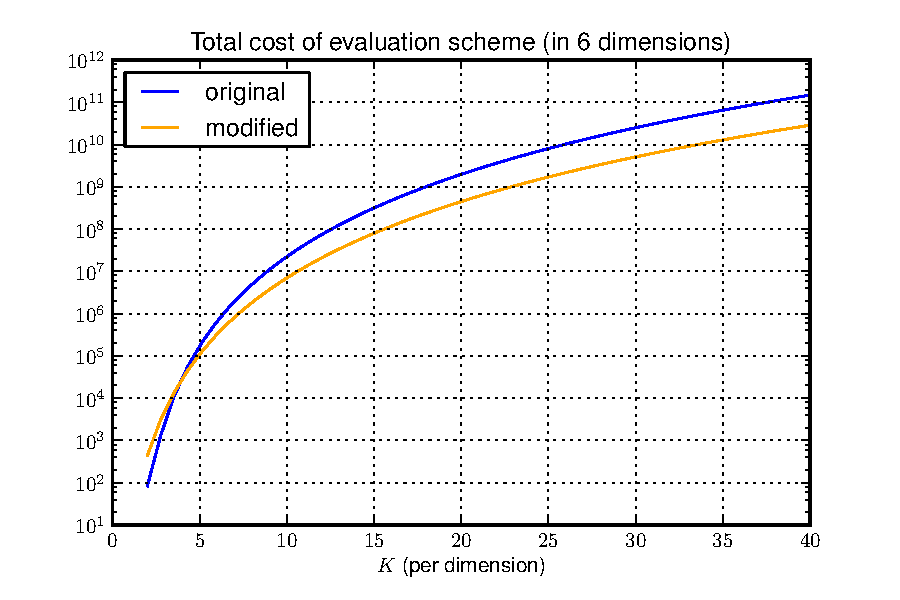
\includegraphics[scale=0.5]{./fig/total_cost_evaluation.pdf}
  \caption{Total cost of a basis evaluation for a hypercubic basis shape
           in $D=6$ dimensions and with $K$ nodes along each direction.}
  \label{fig:total_cost_evaluation}
\end{figure}


\section{Vector-valued wavepackets}


For the purpose of solving the time-dependent Schrödinger equation with non-adiabatic
potentials the scalar wavepackets are not enough. Recall that the potential has $N$
different energy levels. The wavefunction $\Ket{\varphi}$ needs therefore $N$ components
stacked into a vector. In the following we construct \emph{vectorial wavepackets}
where each component is given by a scalar wavepacket. Formally we are in this situation:

\begin{equation}
  \Psi(\vec{x}, t) \assign
  \begin{pmatrix}
    \Phi_0(\vec{x}, t) \\
    \vdots \\
    \Phi_{N-1}(\vec{x}, t)
  \end{pmatrix} \,.
\end{equation}

How many free input parameters does this object have? Each component $\Phi_i$ needs
a set $\Pi_i$ of Hagedorn parameters. (We should write $\Phi_i\left[\Pi_i\right]$
but this becomes lengthy so we drop this soon.) If we use the very same parameter
set $\Pi$ for each component we arrive at what we call a \emph{homogeneous wavepacket}.

\begin{definition}[Homogeneous vectorial wavepacket]
  \begin{equation} \label{eq:vectorial_wavepacket_hom}
    \Ket{\Psi} \assign
    \Psi\left[\Pi\right](\vec{x}, t)
    =
    \begin{pmatrix}
      \Phi_0\left[\Pi\right](\vec{x}, t) \\
      \vdots \\
      \Phi_{N-1}\left[\Pi\right](\vec{x}, t) \\
    \end{pmatrix}
  \end{equation}
  where $\Pi_i \equiv \Pi_j \equiv \Pi \,\forall\, i,j$
\end{definition}

However, at any fixed time each component is independent from all other ones. For
this reason we can choose possibly different sets $\Pi_i$ of parameters for all
$N$ components. By doing this we get an \emph{inhomogeneous wavepacket}, formally
defined as:

\begin{definition}[Inhomogeneous vectorial wavepacket]
  \begin{equation} \label{eq:vectorial_wavepacket_inhom}
    \Ket{\Psi} \assign
    \Psi\left[\Pi_0, \ldots, \Pi_{N-1}\right](\vec{x}, t)
    =
    \begin{pmatrix}
      \Phi_0\left[\Pi_0\right](\vec{x}, t) \\
      \vdots \\
      \Phi_{N-1}\left[\Pi_{N-1}\right](\vec{x}, t) \\
    \end{pmatrix}
  \end{equation}
  where $\Pi_i \neq \Pi_j$ is possible.
\end{definition}

In some applications, for example the spawning approach applied to tunneling
\cite{Gradinaru_semiclassical_tunneling} and the non-adiabatic case
\cite{B_spawning_thesis}, it perfectly makes sense to expand every component
into a different basis of $L^2\left(\mathbb{R}^D\right)$. And since each basis
$\phi_{\vec{k}}$ is essentially fully determined by the parameter set $\Pi$ of
its basis functions $\phi_{\vec{k}}$, this results in different parameter sets
$\Pi_i$ for each component $\Phi_i$.

For some computations we find a more explicit representation of $\Psi$ to be
of greater use. The above definitions can be trivially rewritten as follows by
introducing the unit vectors $\vec{e}^j$ of the canonical basis of $\mathbb{R}^N$.
In the homogeneous case we get:

\begin{equation}
  \Psi\left[\Pi\right](\vec{x}, t) = \sum_{n=0}^{N-1} \vec{e}^n \Phi_n\left[\Pi\right](\vec{x}, t)
\end{equation}

and in the inhomogeneous one:

\begin{equation}
  \Psi\left[\Pi_0,\ldots,\Pi_{N-1}\right](\vec{x}, t) = \sum_{n=0}^{N-1} \vec{e}^n \Phi_n\left[\Pi_n\right](\vec{x}, t) \,.
\end{equation}

We should also note that each component can have an individual basis shape $\mathfrak{K}_n$.
But from now on we will not mention this too often but implicitly assume that each
scalar wavepacket uses the currently best basis shape whatever that means.


\section{Gradient computation}
\label{sec:gradient_computation}


In this section we want to compute the gradient of a scalar wavepacket $\Phi$. More precisely
we find the result of the operator application $-i \varepsilon^2 \nabla \Phi$. From
now on we define the short hand notation $y \assign -i \varepsilon^2 \nabla$. We would
like to have an explicit representation of $y$. Of course it includes just the ordinary
gradient differential operator. But we need a more involved representation allowing us to
easily compute the application of $y$ to a wavepacket of the form given in \eqref{eq:scalar_wavepacket}.
Luckily there is a term of precisely the form of $y$ included in the definition of the
ladder operators in equation \eqref{eq:raising_ops_Dd_explicit}. We proceed by solving the
linear system consisting of the two operator definitions of $\mathcal{L}$ and $\mathcal{R}$
for $y$. We begin by transforming the definition of $\mathcal{R}$ as follows (with the usual
definition of $\theta$):

\begin{align*}
  \mathcal{R} & =  \frac{i}{\sqrt{2\varepsilon^2}} \left( \mat{P}\H (\vec{x}-\vec{q}) - \mat{Q}\H (\vec{y}-\vec{p}) \right) \\
  \mathcal{R} & = \theta \mat{P}\H (\vec{x}-\vec{q}) - \theta \mat{Q}\H (\vec{y}-\vec{p}) \\
  \theta \mat{Q}\H (\vec{y}-\vec{p}) & = -\mathcal{R} + \theta \mat{P}\H (\vec{x}-\vec{q}) \\
  \mat{Q}\H (\vec{y}-\vec{p}) & = -\frac{1}{\theta} \mathcal{R} + \mat{P}\H (\vec{x}-\vec{q}) \,.
\end{align*}

Before we proceed in solving this for $y$ we transform the definition of $\mathcal{L}$
such that we can replace the term $(\vec{x}-\vec{q})$:

\begin{align*}
  \mathcal{L} & = -\theta \mat{P}\T (\vec{x}-\vec{q}) + \theta \mat{Q}\T (\vec{y}-\vec{p}) \\
  \theta \mat{P}\T (\vec{x}-\vec{q}) & = -\mathcal{L} + \theta \mat{Q}\T (\vec{y}-\vec{p}) \\
  \mat{P}\T (\vec{x}-\vec{q}) & = -\frac{1}{\theta}\mathcal{L} + \mat{Q}\T (\vec{y}-\vec{p}) \\
  \vec{x}-\vec{q} & = -\frac{1}{\theta}\mat{P}\Tinv\mathcal{L} + \mat{P}\Tinv\mat{Q}\T (\vec{y}-\vec{p}) \,.
\end{align*}

Then we can plug this into the above equation:

\begin{align*}
  \mat{Q}\H (\vec{y}-\vec{p}) & = -\frac{1}{\theta} \mathcal{R} +
                                  \mat{P}\H \left(-\frac{1}{\theta}\mat{P}\Tinv\mathcal{L} + \mat{P}\Tinv\mat{Q}\T (\vec{y}-\vec{p}) \right) \\
  \mat{Q}\H (\vec{y}-\vec{p}) & = -\frac{1}{\theta} \mathcal{R} +
                                  -\frac{1}{\theta} \mat{P}\H\mat{P}\Tinv\mathcal{L}
                                  +\mat{P}\H\mat{P}\Tinv\mat{Q}\T (\vec{y}-\vec{p}) \\
  \mat{Q}\H \vec{y} - \mat{Q}\H\vec{p} & = -\frac{1}{\theta} \mathcal{R}
                                           -\frac{1}{\theta} \mat{P}\H\mat{P}\Tinv\mathcal{L}
                                           +\mat{P}\H\mat{P}\Tinv\mat{Q}\T \vec{y}
                                           -\mat{P}\H\mat{P}\Tinv\mat{Q}\T\vec{p} \\
  \mat{Q}\H \vec{y} - \mat{P}\H\mat{P}\Tinv\mat{Q}\T \vec{y}
   & = -\frac{1}{\theta} \mathcal{R}
       -\frac{1}{\theta} \mat{P}\H\mat{P}\Tinv\mathcal{L}
       +\mat{Q}\H\vec{p}
       -\mat{P}\H\mat{P}\Tinv\mat{Q}\T\vec{p} \\
  \underbrace{\left(\mat{Q}\H - \mat{P}\H\mat{P}\Tinv\mat{Q}\T\right)}_{**} \vec{y}
   & = -\frac{1}{\theta} \mathcal{R}
       -\frac{1}{\theta} \mat{P}\H\mat{P}\Tinv\mathcal{L}
       +\left(\mat{Q}\H - \mat{P}\H\mat{P}\Tinv\mat{Q}\T\right)\vec{p} \,.
\end{align*}

Our next task is the computation of the subexpression $**$. For this we start again
with the basis relations from \eqref{eq:PQcond_Dd}. For the first one we get:

\begin{align*}
  \mat{Q}\H \mat{P} - \mat{P}\H \mat{Q} & = 2i \id \\
  \mat{Q}\H - \mat{P}\H \mat{Q} \mat{P}\inv & = 2i \mat{P}\inv \\
\end{align*}

and from the second one:

\begin{align*}
  \mat{P}\T \mat{Q} - \mat{Q}\T \mat{P} & = 0 \\
  \mat{Q} - \mat{P}\Tinv \mat{Q}\T \mat{P} & = 0 \\
  \mat{Q} & = \mat{P}\Tinv \mat{Q}\T \mat{P} \,.
\end{align*}

Combining these two results (replacing the second $\mat{Q}$) we obtain:

\begin{align*}
  \mat{Q}\H - \mat{P}\H \mat{P}\Tinv \mat{Q}\T \mat{P} \mat{P}\inv & = 2i \mat{P}\inv \\
  \mat{Q}\H - \mat{P}\H \mat{P}\Tinv \mat{Q}\T & = 2i \mat{P}\inv \,.
\end{align*}

This last line can then be used as a substitution for $**$ above:

\begin{align*}
  2i \mat{P}\inv \vec{y} & = -\frac{1}{\theta} \mathcal{R}
                             -\frac{1}{\theta} \mat{P}\H\mat{P}\Tinv\mathcal{L}
                             +2i \mat{P}\inv \vec{p} \\
  \mat{P}\inv \vec{y} & = -\frac{1}{2i\theta} \mathcal{R}
                          -\frac{1}{2i\theta} \mat{P}\H \mat{P}\Tinv \mathcal{L}
                          +\mat{P}\inv \vec{p} \\
  \vec{y} & = -\frac{1}{2i\theta} \mat{P}\mathcal{R}
                          -\frac{1}{2i\theta} \mat{P} \mat{P}\H \mat{P}\Tinv \mathcal{L}
                          +\vec{p} \,.
\end{align*}

Finally cleaning up and undoing the introduction of $\theta$ we arrive at:

\begin{equation}
  \vec{y} = \sqrt{\frac{\varepsilon^2}{2}} \left( \mat{P}\mathcal{R} + \mat{\conj{P}} \mathcal{L} \right) + \vec{p} \,.
\end{equation}

If we had begun by using the operators $\mathcal{L}$ and $\mathcal{R}$ in the opposite order
we would have got the complex conjugate equation:

\begin{equation}
  \vec{y} = \sqrt{\frac{\varepsilon^2}{2}} \left( \conj{\mat{P}}\mathcal{L} + \mat{P} \mathcal{R} \right) + \vec{p} \,.
\end{equation}

We can simplify the matrix product $\mat{P} \mat{P}\H \mat{P}\Tinv$ to obtain $\mat{\conj{P}}$.
The reason is the conditions \eqref{eq:PQcond_Dd} which must be fulfilled by
$\mat{P}$ and $\mat{Q}$, see \cite{H_ladder_operators}.


\subsection{Applying the gradient operator}


With this explicit representation of the $y$ operator in terms of raising
and lowering operators we can now study its application to an arbitrary
basis function $\phi_{\vec{k}}$. In the end we then need to apply $y$ to the
whole scalar wavepacket $\Phi$ in order to find its kinetic energy.

What do we have to expect when applying $y$ to a basis function $\phi_{\vec{k}}$?
First, we know that the gradient is defined as usual as:

\begin{equation*}
  \nabla_{\vec{x}} \assign
  \begin{pmatrix}
    \pdiff{}{x_0} \\
    \vdots \\
    \pdiff{}{x_{D-1}} \\
  \end{pmatrix} \,.
\end{equation*}

Hence we have to expect that the gradient applied to $\phi_{\vec{k}}:\mathbb{R}^D\rightarrow\mathbb{C}$
is a vector with $D$ components. Next we conclude from \eqref{eq:raising_ops_Dd_vectorial} that the
ladder operators applied to a function give another vector of same shape. We wish to compute:

\begin{equation*}
  y \phi_{\vec{k}}(\vec{x}) = \sqrt{\frac{\varepsilon^2}{2}} \left( \mat{P}\mathcal{R} + \conj{\mat{P}} \mathcal{L} \right) \phi_{\vec{k}}(\vec{x})
                              + \vec{p} \phi_{\vec{k}}(\vec{x})
\end{equation*}

and if we carry out the application of the ladder operators we get step by step
the following relation for the gradient of a single basis function:

\begin{equation*}
  y \phi_{\vec{k}}(\vec{x}) =
  \sqrt{\frac{\varepsilon^2}{2}} \left(
  \mat{P}
    \begin{pmatrix}
      \mathcal{R}_0 \\
      \vdots \\
      \mathcal{R}_{D-1}
    \end{pmatrix}
  + \conj{\mat{P}}
    \begin{pmatrix}
      \mathcal{L}_0 \\
      \vdots \\
      \mathcal{L}_{D-1}
    \end{pmatrix}
  \right) \phi_{\vec{k}}(\vec{x})
  + \vec{p} \phi_{\vec{k}}(\vec{x})
\end{equation*}

where we apply the ladder operators now:

\begin{equation} \label{eq:grad_basis_function_DD}
  y \phi_{\vec{k}}(\vec{x})
  =
  \sqrt{\frac{\varepsilon^2}{2}}
  \left(
    \mat{P}
    \begin{pmatrix}
      \sqrt{k_0 + 1} \phi_{\vec{k}+\vec{e}^0} \\
      \vdots \\
      \sqrt{k_{D-1} + 1} \phi_{\vec{k}+\vec{e}^{D-1}}
    \end{pmatrix}
    +
    \conj{\mat{P}}
    \begin{pmatrix}
      \sqrt{k_0} \phi_{\vec{k}-\vec{e}^0} \\
      \vdots \\
      \sqrt{k_{D-1}} \phi_{\vec{k}-\vec{e}^{D-1}}
    \end{pmatrix}
  \right)
  + \vec{p} \phi_{\vec{k}} \,.
\end{equation}

This is just for one single basis function. But we need more.
Thus we compute the gradient of a whole scalar wavepacket
$\Phi = \sum_{\vec{k}\in\mathfrak{K}} c_{\vec{k}}\phi_{\vec{k}}$:

\begin{equation*}
  y \Phi
  = \sum_{\vec{k}\in\mathfrak{K}} y \, c_{\vec{k}}\phi_{\vec{k}}
  = \sum_{\vec{k}\in\mathfrak{K}} c_{\vec{k}} \, y \phi_{\vec{k}}
\end{equation*}

For a shorter notation we define the following variables:

\begin{align*}
  \theta & \assign \sqrt{\frac{\varepsilon^2}{2}} \\
  \vec{\alpha}(\phi_{\vec{k}}) & \assign
     \begin{pmatrix}
      \sqrt{k_0 + 1} \phi_{\vec{k}+\vec{e}^0} \\
      \vdots \\
      \sqrt{k_{D-1} + 1} \phi_{\vec{k}+\vec{e}^{D-1}}
    \end{pmatrix} \\
  \vec{\beta}(\phi_{\vec{k}}) & \assign
    \begin{pmatrix}
      \sqrt{k_0} \phi_{\vec{k}-\vec{e}^0} \\
      \vdots \\
      \sqrt{k_{D-1}} \phi_{\vec{k}-\vec{e}^{D-1}}
    \end{pmatrix} \,.
\end{align*}

Continuing we derive:

\begin{align*}
  & = \sum_{\vec{k}\in\mathfrak{K}}
        \left(
          c_{\vec{k}} \vec{p} \phi_{\vec{k}}
          + \theta c_{\vec{k}} \mat{P} \vec{\alpha}(\phi_{\vec{k}})
          + \theta c_{\vec{k}} \conj{\mat{P}} \vec{\beta}(\phi_{\vec{k}})
        \right) \nonumber\\
  & = \sum_{\vec{k}\in\mathfrak{K}} c_{\vec{k}} \vec{p} \phi_{\vec{k}}
    + \sum_{\vec{k}\in\mathfrak{K}} \theta c_{\vec{k}} \mat{P} \vec{\alpha}(\phi_{\vec{k}})
    + \sum_{\vec{k}\in\mathfrak{K}} \theta c_{\vec{k}} \conj{\mat{P}} \vec{\beta}(\phi_{\vec{k}}) \,.
\end{align*}

It becomes obvious that $y \phi_{\vec{k}}$ has contributions from all neighbours
$\phi_{\vec{k} + \vec{e}^d}$ and $\phi_{\vec{k} - \vec{e}^d}$ for all $d \in [0, \ldots, D-1]$
and from $\phi_{\vec{k}}$. This immediately raises the question of an efficient
computation. In the end we will need $y \phi_{\vec{k}}$ for all $\vec{k} \in \mathfrak{K}$.
Since there are ladder operators involved we have to be careful for all $\vec{k}$
on the border of $\mathfrak{K}$ who don't have a full set of neighbours in all
directions $d$. For each neighbour $\vec{k}\pm\vec{e}^d$ that is not part of the
basis shape $\mathfrak{K}$ we have to decide what to do. And the rules are as follows.

If the vector $\vec{k}-\vec{e}^d$ has negative components, then we can take the
corresponding basis function to be equivalent zero. We call this situation an
\emph{underflow} \footnote{ This has nothing to do with the usual arithmetic
over/underflow. It just serves as a notation of \emph{where} we access elements
outside of our basis shape $\mathfrak{K}$.}.

The other case is more involved. The functions $\phi_{\vec{k}}$ clearly never
vanish identically zero. However we only have finite linear combinations $\Phi$ of
basis functions $\phi_{\vec{k}}$. Hence all coefficients for sufficiently \emph{large}
$\vec{k}$ vanish. And finally we are only interested in the new coefficients
$c_{\vec{k}}^{\prime i}$ of each component $i$ of the gradient $y \phi_{\vec{k}}$. For
this reason we can also insert zeros in the case such an \emph{overflow} occurs.
For an example of the situation and the issues that may arise refer to figure
\ref{fig:grad_phi_kl_stencil}.

\begin{figure}
  \centering
  \begin{tikzpicture}[%
    func/.style={scale=0.8,color=gray},
    zero/.style={scale=0.8,color=gray}]

    \node[zero, color=black] (v0m1) at (1,0) {$0$};
    \node[zero] (v1m1) at (2,0) {$0$};
    \node[zero] (v2m1) at (3,0) {$0$};
    \node[zero] (v3m1) at (4,0) {$0$};
    \node[zero] (v4m1) at (5,0) {$0$};
    \node[zero] (v5m1) at (6,0) {$0$};
    %\node[zero] (v6m1) at (7,0) {$0$};

    \node[zero, color=black] (vm10) at (0,1) {$0$};
    \node[zero] (vm11) at (0,2) {$0$};
    \node[zero] (vm12) at (0,3) {$0$};
    \node[zero] (vm13) at (0,4) {$0$};
    \node[zero, color=black] (vm14) at (0,5) {$0$};
    %\node[zero] (vm15) at (0,6) {$0$};

    \node[func, color=black] (v00) at (1,1) {$\phi_{0,0}$};
    \node[func, color=black] (v01) at (1,2) {$\phi_{0,1}$};
    \node[func] (v02) at (1,3) {$\phi_{0,2}$};
    \node[func, color=black] (v03) at (1,4) {$\phi_{0,3}$};
    \node[func, color=black] (v04) at (1,5) {$\phi_{0,4}$};
    \node[func, color=black] (v05) at (1,6) {$\phi_{0,5}$};

    \node[func, color=black] (v10) at (2,1) {$\phi_{1,0}$};
    \node[func] (v11) at (2,2) {$\phi_{1,1}$};
    \node[func] (v12) at (2,3) {$\phi_{1,2}$};
    \node[func] (v13) at (2,4) {$\phi_{1,3}$};
    \node[func, color=black] (v14) at (2,5) {$\phi_{1,4}$};
    \node[func] (v15) at (2,6) {$\phi_{1,5}$};

    \node[func] (v20) at (3,1) {$\phi_{2,0}$};
    \node[func] (v21) at (3,2) {$\phi_{2,1}$};
    \node[func, color=black] (v22) at (3,3) {$\phi_{2,2}$};
    \node[func] (v23) at (3,4) {$\phi_{2,3}$};
    \node[func] (v24) at (3,5) {$\phi_{2,4}$};
    \node[func] (v25) at (3,6) {$\phi_{2,5}$};

    \node[func] (v30) at (4,1) {$\phi_{3,0}$};
    \node[func, color=black] (v31) at (4,2) {$\phi_{3,1}$};
    \node[func, color=black] (v32) at (4,3) {$\phi_{3,2}$};
    \node[func, color=black] (v33) at (4,4) {$\phi_{3,3}$};
    \node[func] (v34) at (4,5) {$\phi_{3,4}$};
    \node[func] (v35) at (4,6) {$\phi_{3,5}$};

    \node[func] (v40) at (5,1) {$\phi_{4,0}$};
    \node[func] (v41) at (5,2) {$\phi_{4,1}$};
    \node[func, color=black] (v42) at (5,3) {$\phi_{4,2}$};
    \node[func] (v43) at (5,4) {$\phi_{4,3}$};
    \node[func, color=black] (v44) at (5,5) {$\phi_{4,4}$};
    \node[func] (v45) at (5,6) {$\phi_{4,5}$};

    \node[func] (v50) at (6,1) {$\phi_{5,0}$};
    \node[func] (v51) at (6,2) {$\phi_{5,1}$};
    \node[func] (v52) at (6,3) {$\phi_{5,2}$};
    \node[func, color=black] (v53) at (6,4) {$\phi_{5,3}$};
    \node[func, color=black] (v54) at (6,5) {$\phi_{5,4}$};
    \node[func, color=black] (v55) at (6,6) {$\phi_{5,5}$};

    \node[func] (v60) at (7,1) {$\phi_{6,0}$};
    \node[func] (v61) at (7,2) {$\phi_{6,1}$};
    \node[func] (v62) at (7,3) {$\phi_{6,2}$};
    \node[func] (v63) at (7,4) {$\phi_{6,3}$};
    \node[func, color=black] (v64) at (7,5) {$\phi_{6,4}$};
    %\node[func] (v65) at (7,6) {$\phi_{6,5}$};

    \begin{scope}
    \draw[draw=black,line width=0.7pt] ($(v00)+(0.0,-0.5)$)
        to[out=0,in=180] ($(v50)+(0.0,-0.5)$)
        to[out=0,in=270] ($(v50)+(0.5,0.0)$)
        to[out=90,in=270] ($(v54)+(0.5,0.0)$)
        to[out=90,in=0] ($(v54)+(0.0,0.5)$)
        to[out=180,in=0] ($(v04)+(0.0,0.5)$)
        to[out=180,in=90] ($(v04)+(-0.5,0.0)$)
        to[out=270,in=90] ($(v00)+(-0.5,0.0)$)
        to[out=270,in=180] ($(v00)+(0.0,-0.5)$);
    \end{scope}

    % lower left
    \begin{scope}
    \draw[draw=blue!100,line width=0.8pt] ($(vm10)+(0.0,0.3)$)
        to[out=170,in=90] ($(vm10)+(-0.3,0.0)$)
        to[out=270,in=190] ($(vm10)+(0.0,-0.3)$)
        to[out=10,in=80] ($(v0m1)+(-0.3,0.0)$)
        to[out=260,in=180] ($(v0m1)+(0.0,-0.3)$)
        to[out=0,in=280] ($(v0m1)+(0.3,0.0)$)
        to[out=100,in=350] ($(vm10)+(0.0,0.3)$);
    \end{scope}
    \begin{scope}
    \draw[draw=orange!100,line width=0.8pt] ($(v10)-(0.0,0.3)$)
        to[out=10,in=170] ($(v10)-(0.0,0.3)$)
        to[out=0,in=270] ($(v10)-(-0.3,0.0)$)
        to[out=90,in=10] ($(v10)-(0.0,-0.3)$)
        to[out=190,in=260] ($(v01)-(-0.3,0.0)$)
        to[out=80,in=0] ($(v01)-(0.0,-0.3)$)
        to[out=180,in=100] ($(v01)-(0.3,0.0)$)
        to[out=280,in=170] ($(v10)-(0.0,0.3)$);
    \end{scope}
    \begin{scope}
    \draw[draw=gray!100,line width=0.8pt] ($(v00)-(0.0,0.3)$)
        to[out=180,in=270] ($(v00)-(0.3,0.0)$)
        to[out=90,in=180] ($(v00)+(0.0,0.3)$)
        to[out=0,in=90] ($(v00)+(0.3,0.0)$)
        to[out=270,in=0] ($(v00)-(0.0,0.3)$);
    \end{scope}

    % upper left
    \begin{scope}
    \draw[draw=blue!100,line width=0.8pt] ($(vm14)+(0.0,0.3)$)
        to[out=170,in=90] ($(vm14)+(-0.3,0.0)$)
        to[out=270,in=190] ($(vm14)+(0.0,-0.3)$)
        to[out=10,in=80] ($(v03)+(-0.3,0.0)$)
        to[out=260,in=180] ($(v03)+(0.0,-0.3)$)
        to[out=0,in=280] ($(v03)+(0.3,0.0)$)
        to[out=100,in=350] ($(vm14)+(0.0,0.3)$);
    \end{scope}
    \begin{scope}
    \draw[draw=orange!100,line width=0.8pt] ($(v14)-(0.0,0.3)$)
        to[out=10,in=170] ($(v14)-(0.0,0.3)$)
        to[out=0,in=270] ($(v14)-(-0.3,0.0)$)
        to[out=90,in=10] ($(v14)-(0.0,-0.3)$)
        to[out=190,in=260] ($(v05)-(-0.3,0.0)$)
        to[out=80,in=0] ($(v05)-(0.0,-0.3)$)
        to[out=180,in=100] ($(v05)-(0.3,0.0)$)
        to[out=280,in=170] ($(v14)-(0.0,0.3)$);
    \end{scope}
    \begin{scope}
    \draw[draw=gray!100,line width=0.8pt] ($(v04)-(0.0,0.3)$)
        to[out=180,in=270] ($(v04)-(0.3,0.0)$)
        to[out=90,in=180] ($(v04)+(0.0,0.3)$)
        to[out=0,in=90] ($(v04)+(0.3,0.0)$)
        to[out=270,in=0] ($(v04)-(0.0,0.3)$);
    \end{scope}

    % upper right
    \begin{scope}
    \draw[draw=blue!100,line width=0.8pt] ($(v44)+(0.0,0.3)$)
        to[out=170,in=90] ($(v44)+(-0.3,0.0)$)
        to[out=270,in=190] ($(v44)+(0.0,-0.3)$)
        to[out=10,in=80] ($(v53)+(-0.3,0.0)$)
        to[out=260,in=180] ($(v53)+(0.0,-0.3)$)
        to[out=0,in=280] ($(v53)+(0.3,0.0)$)
        to[out=100,in=350] ($(v44)+(0.0,0.3)$);
    \end{scope}
    \begin{scope}
    \draw[draw=orange!100,line width=0.8pt] ($(v64)-(0.0,0.3)$)
        to[out=10,in=170] ($(v64)-(0.0,0.3)$)
        to[out=0,in=270] ($(v64)-(-0.3,0.0)$)
        to[out=90,in=10] ($(v64)-(0.0,-0.3)$)
        to[out=190,in=260] ($(v55)-(-0.3,0.0)$)
        to[out=80,in=0] ($(v55)-(0.0,-0.3)$)
        to[out=180,in=100] ($(v55)-(0.3,0.0)$)
        to[out=280,in=170] ($(v64)-(0.0,0.3)$);
    \end{scope}
    \begin{scope}
    \draw[draw=gray!100,line width=0.8pt] ($(v54)-(0.0,0.3)$)
        to[out=180,in=270] ($(v54)-(0.3,0.0)$)
        to[out=90,in=180] ($(v54)+(0.0,0.3)$)
        to[out=0,in=90] ($(v54)+(0.3,0.0)$)
        to[out=270,in=0] ($(v54)-(0.0,0.3)$);
    \end{scope}

    % central
    \begin{scope}
    \draw[draw=blue!100,line width=0.8pt] ($(v22)+(0.0,0.3)$)
        to[out=170,in=90] ($(v22)+(-0.3,0.0)$)
        to[out=270,in=190] ($(v22)+(0.0,-0.3)$)
        to[out=10,in=80] ($(v31)+(-0.3,0.0)$)
        to[out=260,in=180] ($(v31)+(0.0,-0.3)$)
        to[out=0,in=280] ($(v31)+(0.3,0.0)$)
        to[out=100,in=350] ($(v22)+(0.0,0.3)$);
    \end{scope}
    \begin{scope}
    \draw[draw=orange!100,line width=0.8pt] ($(v42)-(0.0,0.3)$)
        to[out=10,in=170] ($(v42)-(0.0,0.3)$)
        to[out=0,in=270] ($(v42)-(-0.3,0.0)$)
        to[out=90,in=10] ($(v42)-(0.0,-0.3)$)
        to[out=190,in=260] ($(v33)-(-0.3,0.0)$)
        to[out=80,in=0] ($(v33)-(0.0,-0.3)$)
        to[out=180,in=100] ($(v33)-(0.3,0.0)$)
        to[out=280,in=170] ($(v42)-(0.0,0.3)$);
    \end{scope}
    \begin{scope}
    \draw[draw=gray!100,line width=0.8pt] ($(v32)-(0.0,0.3)$)
        to[out=180,in=270] ($(v32)-(0.3,0.0)$)
        to[out=90,in=180] ($(v32)+(0.0,0.3)$)
        to[out=0,in=90] ($(v32)+(0.3,0.0)$)
        to[out=270,in=0] ($(v32)-(0.0,0.3)$);
    \end{scope}
\end{tikzpicture}

  \caption[Computing the gradient in two dimensions] {Stencil application for
           computing the gradient $y \phi_{\vec{k}}$ for different $\vec{k}$ in
           two dimensions. For each computation we need the function itself
           (grey circles), the backward neighbours $\phi_{\vec{k}-\vec{e}^d}$
           (blue contours) and the forward neighbours $\phi_{\vec{k}+\vec{e}^d}$
           (orange contours). Clearly we need additional functions outside of
           the basis shape $\mathfrak{K}$ (black rectangle). In all corners
            and along all sides we under- and overflow respectively.}
  \label{fig:grad_phi_kl_stencil}
\end{figure}

Before we continue let's make a not so small but very simple example. Assume
the hypercubic basis shape in two dimensions is $\mathfrak{K} = \vec{K} = (3,3)$.
The wavepacket consists of the following linear combination:

\begin{align*}
  \Phi \assign \, & c_{0,0} \phi_{0,0} + c_{1,0} \phi_{1,0} + c_{2,0} \phi_{2,0} \\
             + \, & c_{0,1} \phi_{0,1} + c_{1,1} \phi_{1,1} + c_{2,1} \phi_{2,1} \\
             + \, & c_{0,2} \phi_{0,2} + c_{1,2} \phi_{1,2} + c_{2,2} \phi_{2,2} \,.
\end{align*}

Computing the gradients individually for some of the terms we get:

\begin{center}
\begin{tabular}{ll}
Multi-index node  & Gradient \\
\hline \\
$\vec{k} = (0,0)$ & $c_{0,0} \, \vec{p} \phi_{0,0} +
                     \theta c_{0,0} \, \mat{P} \begin{pmatrix} \sqrt{1} \, \phi_{1,0} \\
                                                               \sqrt{1} \, \phi_{0,1}
                                               \end{pmatrix} +
                     \theta c_{0,0} \, \conj{\mat{P}} \begin{pmatrix} \sqrt{0} \, \phi_{-1,0} \\
                                                                      \sqrt{0} \, \phi_{0,-1}
                                                      \end{pmatrix}$\\
$\vec{k} = (1,0)$ & $c_{1,0} \, \vec{p} \phi_{1,0} +
                     \theta c_{1,0} \, \mat{P} \begin{pmatrix} \sqrt{2} \, \phi_{2,0} \\
                                                               \sqrt{1} \, \phi_{1,1}
                                               \end{pmatrix} +
                     \theta c_{1,0} \, \conj{\mat{P}} \begin{pmatrix} \sqrt{1} \, \phi_{0,0} \\
                                                                      \sqrt{0} \, \phi_{1,-1}
                                                      \end{pmatrix}$\\
$\vec{k} = (0,1)$ & $c_{0,1} \, \vec{p} \phi_{0,1} +
                     \theta c_{0,1} \, \mat{P} \begin{pmatrix} \sqrt{1} \, \phi_{1,1} \\
                                                               \sqrt{2} \, \phi_{0,2}
                                               \end{pmatrix} +
                     \theta c_{0,1} \, \conj{\mat{P}} \begin{pmatrix} \sqrt{0} \, \phi_{-1,1} \\
                                                                      \sqrt{1} \, \phi_{0,0}
                                                      \end{pmatrix}$\\
$\vec{k} = (1,1)$ & $c_{1,1} \, \vec{p} \phi_{1,1} +
                     \theta c_{1,1} \, \mat{P} \begin{pmatrix} \sqrt{2} \, \phi_{2,1} \\
                                                               \sqrt{2} \, \phi_{1,2}
                                               \end{pmatrix} +
                     \theta c_{1,1} \, \conj{\mat{P}} \begin{pmatrix} \sqrt{1} \, \phi_{0,1} \\
                                                                      \sqrt{1} \, \phi_{1,0}
                                                      \end{pmatrix}$ \\
$\vec{k} = (2,1)$ & $c_{2,1} \, \vec{p} \phi_{2,1} +
                     \theta c_{2,1} \, \mat{P} \begin{pmatrix} \sqrt{3} \, \phi_{3,1} \\
                                                               \sqrt{2} \, \phi_{2,2}
                                               \end{pmatrix} +
                     \theta c_{2,1} \, \conj{\mat{P}} \begin{pmatrix} \sqrt{2} \, \phi_{1,1} \\
                                                                      \sqrt{1} \, \phi_{2,0}
                                                      \end{pmatrix}$ \\
$\vec{k} = (1,2)$ & $c_{1,2} \, \vec{p} \phi_{1,2} +
                     \theta c_{1,2} \, \mat{P} \begin{pmatrix} \sqrt{2} \, \phi_{2,2} \\
                                                               \sqrt{3} \, \phi_{1,3}
                                               \end{pmatrix} +
                     \theta c_{1,2} \, \conj{\mat{P}} \begin{pmatrix} \sqrt{1} \, \phi_{0,2} \\
                                                                      \sqrt{2} \, \phi_{1,1}
                                                      \end{pmatrix}$ \\
$\vdots$ & $\hdots$
\end{tabular}
\end{center}

and we would sum up all these terms to get the overall gradient of $\Phi$. In this form however
it is not of much use to us. We want to represent the gradient again as linear combinations
over the same set of basis functions:

\begin{equation} \label{eq:gradient_basis_expandion}
  y \Phi = \sum_{\vec{k} \in \overline{\mathfrak{K}}} \vec{c}^\prime_{\vec{k}} \phi_{\vec{k}}
\end{equation}

where $\vec{c}^\prime_{\vec{k}} \in \mathbb{C}^{D}$ and $\overline{\mathfrak{K}}$ is the
extended basis shape (in case of our example $\overline{\mathfrak{K}} = \vec{K}^\prime = (4,4)$).
This is indeed possible, expanding the fourth row from the table above in
instances of $\phi_{\vec{k}}$ and summing up we get:

\begin{equation*}
    c_{1,1} \, \vec{p} \phi_{1,1}
  + \theta c_{1,1} \, \sqrt{2} \, \mat{P}_{:,0} \phi_{2,1}
  + \theta c_{1,1} \, \sqrt{2} \, \mat{P}_{:,1} \phi_{1,2}
  + \theta c_{1,1} \, \conj{\mat{P}}_{:,0} \phi_{0,1}
  + \theta c_{1,1} \, \conj{\mat{P}}_{:,1} \phi_{1,0} \,.
\end{equation*}

In finding the coefficient $\vec{c}_{1,1}$ of $\phi_{1,1}$ we have to be very careful, because
there are further terms on up to 4 other rows that contribute to $\vec{c}_{1,1}$.
(Note that this coefficient is a good example as its lattice node has a full set
of 4 neighbours.) Summing up all relevant terms we find that:

\begin{equation*}
  \vec{c}^\prime_{1,1} = c_{1,1} \, \vec{p}
+ \theta c_{0,1} \, \mat{P}_{:,0} \,.
+ \theta c_{1,0} \, \mat{P}_{:,1}
+ \theta c_{2,1} \, \sqrt{2} \, \conj{\mat{P}}_{:,0}
+ \theta c_{1,2} \, \sqrt{2} \, \conj{\mat{P}}_{:,1} \,.
\end{equation*}

The last four terms can be recombined into one per pair and we end up with:

\begin{equation*}
  \vec{c}^\prime_{1,1} = c_{1,1} \, \vec{p}
+ \theta \mat{P}
  \begin{pmatrix}
    c_{0,1} \\ c_{1,0}
  \end{pmatrix}
+ \theta \conj{\mat{P}}
  \begin{pmatrix}
    \sqrt{2} \, c_{2,1} \\ \sqrt{2} \, c_{1,2}
  \end{pmatrix}
\end{equation*}

Doing these transformations in a systematic way is the major issue in computing the gradients.
With a bit of guessing we can find the following general rule for the coefficient vectors
$\vec{c}^\prime_{\vec{k}}$ for all $\vec{k} \in \overline{\mathfrak{K}}$:

\begin{equation*}
  \vec{c}^\prime_{\vec{k}} = c_{\vec{k}} \, \vec{p}
                             + \sqrt{\frac{\varepsilon^2}{2}} \sum_{d=0}^{D-1} c_{\vec{k}+\vec{e}^d} \, \sqrt{\vec{k}_{d}+1} \, \conj{\mat{P}}_{:,d}
                             + \sqrt{\frac{\varepsilon^2}{2}} \sum_{d=0}^{D-1} c_{\vec{k}-\vec{e}^d} \, \sqrt{\vec{k}_{d}} \, \mat{P}_{:,d}
\end{equation*}

which again can be cast in compact form:

\begin{equation} \label{eq:gradient_coefficients_DD}
  \vec{c}^\prime_{\vec{k}} = c_{\vec{k}} \, \vec{p}
                             + \sqrt{\frac{\varepsilon^2}{2}} \left(
                               \conj{\mat{P}}
                               \begin{pmatrix}
                                 c_{\vec{k}+\vec{e}^0} \, \sqrt{\vec{k}_{0}+1} \\
                                 \vdots \\
                                 c_{\vec{k}+\vec{e}^{D-1}} \, \sqrt{\vec{k}_{D-1}+1}
                               \end{pmatrix}
                             + \mat{P}
                               \begin{pmatrix}
                                 c_{\vec{k}-\vec{e}^0} \, \sqrt{\vec{k}_{0}} \\
                                 \vdots \\
                                 c_{\vec{k}-\vec{e}^{D-1}} \, \sqrt{\vec{k}_{D-1}}
                               \end{pmatrix}
                               \right) \,.
\end{equation}


\subsection{Gather-type algorithm}


The most simple algorithm to compute $y \phi_{\vec{k}}$ for all $\vec{k} \in \mathfrak{K}$
has to iterate over all $\vec{k} \in \overline{\mathfrak{K}}$ and apply the
two stencils to get the data from backward and forward neighbours of $\vec{k}$
and to compute $y \phi_{\vec{k}}$ by the formula \eqref{eq:gradient_coefficients_DD}.
This is simple to understand and works reasonably efficient. We call this algorithm the
\emph{gather-type} stencil application.

The only not so easy point here is that we can not iterate just over $\mathfrak{K}$
but have to extend the basis shape due to the nature of the neighbourhood stencil.
In more detail, this is necessary as there are $\vec{k}^\prime \notin \mathfrak{K}$
for which the above formula \eqref{eq:gradient_coefficients_DD} still yields a non-zero result since
the stencil centred at $\vec{k}^\prime$ still overlaps with the basis shape $\mathfrak{K}$.
And we do not want to loose these contributions. Therefore we extend the basis shape
$\mathfrak{K}$ by one node in all directions and get what we denote by $\overline{\mathfrak{K}}$.
This should be clear by looking at figure \ref{fig:grad_phi_kl_stencil}.

In one single space dimension $x$ the gradient equals the derivative and the result
is not a vector of functions but just a function too. Therefore it is easier to
understand the gradient computation for one-dimensional wavepackets $\Phi(x)$ first.
The whole process of the gather-type algorithm is shown in figure
\ref{fig:grad_phi_kl_gather_stencil_1D} in considerable detail.

\begin{figure}
  \centering
  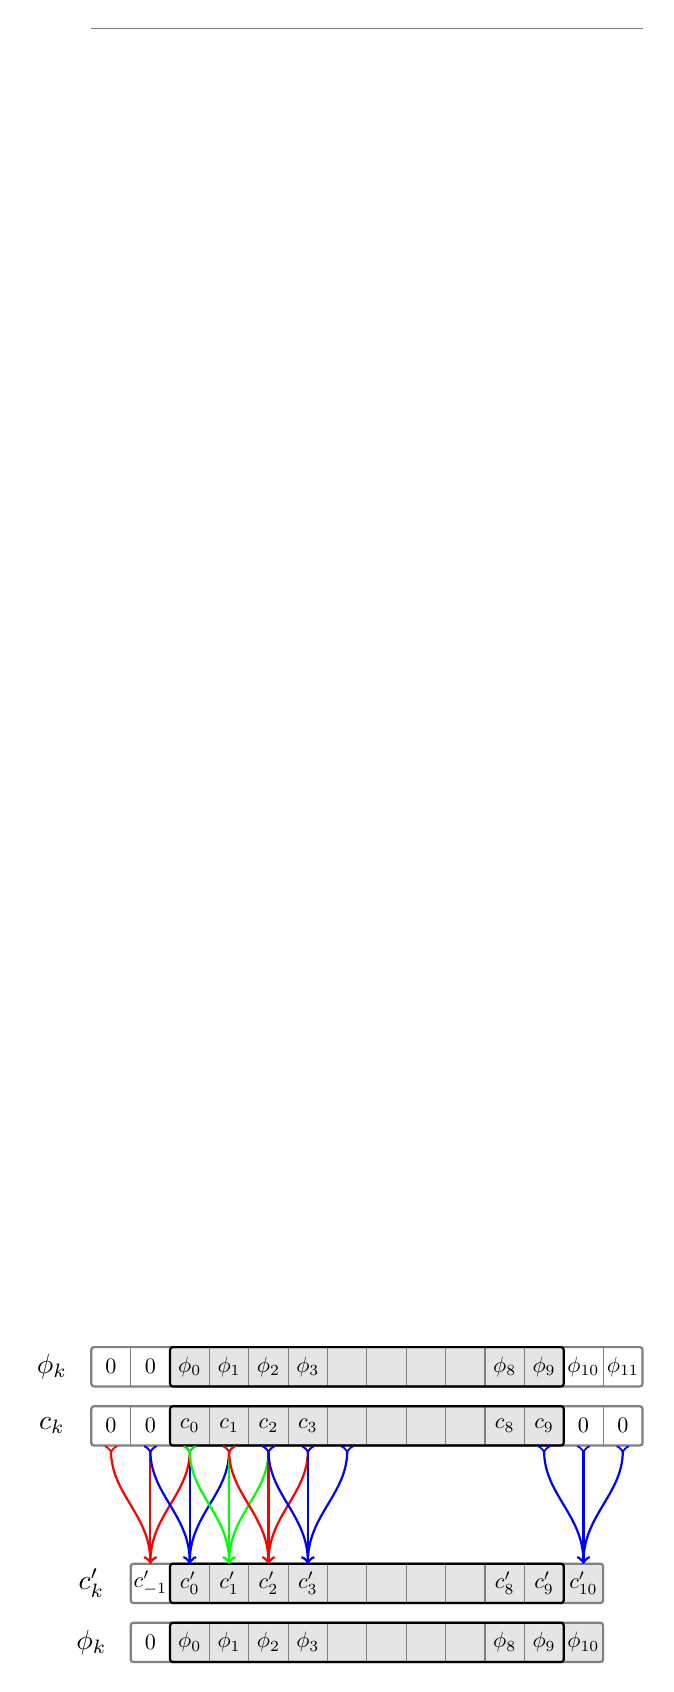
\begin{tikzpicture}
  \coordinate (com2) at (-0.75, 2.0);
  \coordinate (com1) at (-0.25, 2.0);
  \coordinate (co0) at (0.25, 2.0);
  \coordinate (co1) at (0.75, 2.0);
  \coordinate (co2) at (1.25, 2.0);
  \coordinate (co3) at (1.75, 2.0);
  \coordinate (co4) at (2.25, 2.0);
  \coordinate (co5) at (2.75, 2.0);
  \coordinate (co6) at (3.25, 2.0);
  \coordinate (co9) at (4.75, 2.0);
  \coordinate (co10) at (5.25, 2.0);
  \coordinate (co11) at (5.75, 2.0);

  \coordinate (cpm1) at (-0.25, 0.5);
  \coordinate (cp0) at (0.25, 0.5);
  \coordinate (cp1) at (0.75, 0.5);
  \coordinate (cp2) at (1.25, 0.5);
  \coordinate (cp3) at (1.75, 0.5);
  \coordinate (cp4) at (2.25, 0.5);
  \coordinate (cp5) at (2.75, 0.5);
  \coordinate (cp6) at (3.25, 0.5);
  \coordinate (cp8) at (4.25, 0.5);
  \coordinate (cp9) at (4.75, 0.5);
  \coordinate (cp10) at (5.25, 0.5);

  % upper
  \fill[gray!20, rounded corners=1] (0.0,2.75) rectangle (5.0,3.25);
  \draw[step=5mm, ystep=20cm, gray] (-1.0,2.75) grid (6.0,3.25);
  \draw[gray, thick, rounded corners=1] (-1.0,2.75) rectangle (6.0,3.25);
  \draw[black, thick, rounded corners=1] (0.0,2.75) rectangle (5.0,3.25);

  \fill[gray!20, rounded corners=1] (0.0,2.0) rectangle (5.0,2.5);
  \draw[step=5mm, gray] (-1.0,2.0) grid (6.0,2.5);
  \draw[gray, thick, rounded corners=1] (-1.0,2.0) rectangle (6.0,2.5);
  \draw[black, thick, rounded corners=1] (0.0,2.0) rectangle (5.0,2.5);

  % lower
  \fill[gray!20, rounded corners=1] (0.0,-0.75) rectangle (5.5,-0.25);
  \draw[step=5mm, ystep=20cm, gray] (0.0,-0.75) grid (5.0,-0.25);
  \draw[gray, thick, rounded corners=1] (-0.5,-0.75) rectangle (5.5,-0.25);
  \draw[black, thick, rounded corners=1] (0.0,-0.75) rectangle (5.0,-0.25);

  \fill[gray!20, rounded corners=1] (0.0,0.0) rectangle (5.5,0.5);
  \draw[step=5mm, gray] (0.0,0.0) grid (5.0,0.5);
  \draw[gray, thick, rounded corners=1] (-0.5,0.0) rectangle (5.5,0.5);
  \draw[black, thick, rounded corners=1] (0.0,0.0) rectangle (5.0,0.5);

  \draw[>->, thick, color=red] (com2) to[out=270,in=90] (cpm1);
  \draw[>->, thick, color=red] (com1) to[out=270,in=90] (cpm1);
  \draw[>->, thick, color=red] (co0) to[out=270,in=90] (cpm1);

  \draw[>->, thick, color=blue] (com1) to[out=270,in=90] (cp0);
  \draw[>->, thick, color=blue] (co0) to[out=270,in=90] (cp0);
  \draw[>->, thick, color=blue] (co1) to[out=270,in=90] (cp0);

  \draw[>->, thick, color=green] (co0) to[out=270,in=90] (cp1);
  \draw[>->, thick, color=green] (co1) to[out=270,in=90] (cp1);
  \draw[>->, thick, color=green] (co2) to[out=270,in=90] (cp1);

  \draw[>->, thick, color=red] (co1) to[out=270,in=90] (cp2);
  \draw[>->, thick, color=red] (co2) to[out=270,in=90] (cp2);
  \draw[>->, thick, color=red] (co3) to[out=270,in=90] (cp2);

  \draw[>->, thick, color=blue] (co2) to[out=270,in=90] (cp3);
  \draw[>->, thick, color=blue] (co3) to[out=270,in=90] (cp3);
  \draw[>->, thick, color=blue] (co4) to[out=270,in=90] (cp3);

  \draw[>->, thick, color=blue] (co9) to[out=270,in=90] (cp10);
  \draw[>->, thick, color=blue] (co10) to[out=270,in=90] (cp10);
  \draw[>->, thick, color=blue] (co11) to[out=270,in=90] (cp10);

  \node[scale=0.8] at (-0.75,2.25) [black] {$0$};
  \node[scale=0.8] at (-0.25,2.25) [black] {$0$};
  \node[scale=0.8] at (0.25,2.25) [black] {$c_0$};
  \node[scale=0.8] at (0.75,2.25) [black] {$c_1$};
  \node[scale=0.8] at (1.25,2.25) [black] {$c_2$};
  \node[scale=0.8] at (1.75,2.25) [black] {$c_3$};
  \node[scale=0.8] at (4.25,2.25) [black] {$c_8$};
  \node[scale=0.8] at (4.75,2.25) [black] {$c_9$};
  \node[scale=0.8] at (5.25,2.25) [black] {$0$};
  \node[scale=0.8] at (5.75,2.25) [black] {$0$};

  \node[scale=0.8] at (-0.25,0.25) [black] {$c^\prime_{-1}$};
  \node[scale=0.8] at (0.25,0.25) [black] {$c^\prime_0$};
  \node[scale=0.8] at (0.75,0.25) [black] {$c^\prime_1$};
  \node[scale=0.8] at (1.25,0.25) [black] {$c^\prime_2$};
  \node[scale=0.8] at (1.75,0.25) [black] {$c^\prime_3$};
  \node[scale=0.8] at (4.25,0.25) [black] {$c^\prime_8$};
  \node[scale=0.8] at (4.75,0.25) [black] {$c^\prime_9$};
  \node[scale=0.8] at (5.25,0.25) [black] {$c^\prime_{10}$};

  \node[scale=0.8] at (-0.75,3.0) [black] {$0$};
  \node[scale=0.8] at (-0.25,3.0) [black] {$0$};
  \node[scale=0.8] at (0.25,3.0) [black] {$\phi_0$};
  \node[scale=0.8] at (0.75,3.0) [black] {$\phi_1$};
  \node[scale=0.8] at (1.25,3.0) [black] {$\phi_2$};
  \node[scale=0.8] at (1.75,3.0) [black] {$\phi_3$};
  \node[scale=0.8] at (4.25,3.0) [black] {$\phi_8$};
  \node[scale=0.8] at (4.75,3.0) [black] {$\phi_9$};
  \node[scale=0.8] at (5.25,3.0) [black] {$\phi_{10}$};
  \node[scale=0.8] at (5.75,3.0) [black] {$\phi_{11}$};

  \node[scale=0.8] at (-0.25,-0.5) [black] {$0$};
  \node[scale=0.8] at (0.25,-0.5) [black] {$\phi_0$};
  \node[scale=0.8] at (0.75,-0.5) [black] {$\phi_1$};
  \node[scale=0.8] at (1.25,-0.5) [black] {$\phi_2$};
  \node[scale=0.8] at (1.75,-0.5) [black] {$\phi_3$};
  \node[scale=0.8] at (4.25,-0.5) [black] {$\phi_8$};
  \node[scale=0.8] at (4.75,-0.5) [black] {$\phi_9$};
  \node[scale=0.8] at (5.25,-0.5) [black] {$\phi_{10}$};

  \node at (-1.5,3.0) [black] {$\phi_{k}$};
  \node at (-1.0,-0.5) [black] {$\phi_{k}$};
  \node at (-1.5,2.25) [black] {$c_{k}$};
  \node at (-1.0,0.25) [black] {$c^\prime_{k}$};
\end{tikzpicture}

  \caption[Gather-type stencil in 1D] {The gather-type stencil application for
           computing the gradient $y\Phi$. The upper two arrays show the initial linear
           combination $\Phi$ consisting of basis functions $\phi_k$ and coefficients $c_k$.
           The lower two arrays show the linear combination of $\diff{\Phi}{x}$ consisting
           of the same basis functions $\phi_k$ and new coefficients $c_k^\prime$.
           Each of the triple arrows is one single stencil application (formula
           \eqref{eq:gradient_coefficients_DD}), not all applications are shown.
           We see that the basis shape $\overline{\mathfrak{K}}$ for the gradient
           is larger. And also that we access several elements not part of the original
           basis shape $\mathfrak{K}$. During the computation we insert the zeros
           on the fly and we drop the coefficient $c_{-1}^\prime$ (because $\phi_{-1} \equiv 0$).
           The original basis shape $\mathfrak{K}$ is represented by the black rectangle
           and the actual basis shapes are shown shaded grey.}
  \label{fig:grad_phi_kl_gather_stencil_1D}
\end{figure}

The next figure \ref{fig:grad_phi_kl_gather_stencil_2D} shows the same
algorithm but this time for a two-dimensional wavepacket. It should now be
clear what happens. The principle is the same for an arbitrary number
$D$ of space dimensions and arbitrary basis shapes $\mathfrak{K}$.

\begin{figure}
  \centering
  \begin{tikzpicture}[scale=1,every node/.style={minimum size=0.5cm},on grid]

  \begin{scope}[
      yshift=-100,
      every node/.append style={yslant=0.5, xslant=-1.3},
      yslant=0.5,
      xslant=-1.3
    ]
    \coordinate (c42) at (2.25, 1.25);
    \coordinate (c32) at (1.75, 1.25);
    \coordinate (c22) at (1.25, 1.25);
    \coordinate (c33) at (1.75, 1.75);
    \coordinate (c31) at (1.75, 0.75);

    \coordinate (co15) at (0.75, 2.75);
    \coordinate (co25) at (1.25, 2.75);
    \coordinate (co35) at (1.75, 2.75);
    \coordinate (co24) at (1.25, 2.25);
    \coordinate (co26) at (1.25, 3.25);

    \coordinate (co51) at (2.75, 0.75);
    \coordinate (co61) at (3.25, 0.75);
    \coordinate (co71) at (3.75, 0.75);
    \coordinate (co60) at (3.25, 0.25);
    \coordinate (co62) at (3.25, 1.25);
  \end{scope}

  \begin{scope}[
      yshift=-180,
      every node/.append style={yslant=0.5, xslant=-1.3},
      yslant=0.5,
      xslant=-1.3
    ]
    \coordinate (cp32) at (1.75, 1.25);
    \coordinate (cop25) at (1.25, 2.75);
    \coordinate (cop61) at (3.25, 0.75);
  \end{scope}

  % lower plane
  \begin{scope}[
      yshift=-180,
      every node/.append style={yslant=0.5, xslant=-1.3},
      yslant=0.5,
      xslant=-1.3
    ]
    \draw[step=5mm, thin, gray] (-0.5,-0.5) grid (3.5,3.5);

    \fill[blue!60] (1.5,1) rectangle (2.0,1.5);
    \node at (cp32) [draw, color=blue] {};%{$c^\prime_{3,2}$};

    \fill[orange!60] (1.0,2.5) rectangle (1.5,3.0);
    \node at (cop25) [draw, color=orange] {};%{$c^\prime_{2,5}$};

    \fill[green!80] (3.0,0.5) rectangle (3.5,1.0);
    \node at (cop61) [draw, color=green] {};%{$c^\prime_{6,1}$};

    \draw[black,thick, rounded corners=1] (0,0) rectangle (3,3);
    \draw[gray,thick, rounded corners=1] (-0.5,-0.5) rectangle (3.5,3.5);
  \end{scope}

  % arrows
  \begin{scope}
    \draw[>->, thick] (c31) node[left,scale=1.3] {} to[out=270,in=90] (cp32);
    \draw[>->, thick] (c32) node[left,scale=1.3] {} to[out=270,in=90] (cp32);
    \draw[>->, thick] (c33) node[left,scale=1.3] {} to[out=270,in=90] (cp32);
    \draw[>->, thick] (c22) node[left,scale=1.3] {} to[out=270,in=90] (cp32);
    \draw[>->, thick] (c42) node[left,scale=1.3] {} to[out=270,in=90] (cp32);

    \draw[>->, thick] (co24) node[left,scale=1.3] {} to[out=270,in=90] (cop25);
    \draw[>->, thick] (co25) node[left,scale=1.3] {} to[out=270,in=90] (cop25);
    \draw[>->, thick] (co26) node[left,scale=1.3] {} to[out=270,in=90] (cop25);
    \draw[>->, thick] (co15) node[left,scale=1.3] {} to[out=270,in=90] (cop25);
    \draw[>->, thick] (co35) node[left,scale=1.3] {} to[out=270,in=90] (cop25);

    \draw[>->, thick] (co51) node[left,scale=1.3] {} to[out=270,in=90] (cop61);
    \draw[>->, thick] (co61) node[left,scale=1.3] {} to[out=270,in=90] (cop61);
    \draw[>->, thick] (co71) node[left,scale=1.3] {} to[out=270,in=90] (cop61);
    \draw[>->, thick] (co62) node[left,scale=1.3] {} to[out=270,in=90] (cop61);
    \draw[>->, thick] (co60) node[left,scale=1.3] {} to[out=270,in=90] (cop61);
  \end{scope}

  % upper plane
  \begin{scope}[
      yshift=-100,
      every node/.append style={yslant=0.5, xslant=-1.3},
      yslant=0.5,
      xslant=-1.3
    ]
    \fill[white,fill opacity=0.8] (-1.0,-1.0) rectangle (4.0,4.0);
    \draw[step=5mm, thin, gray] (-1.0,-1.0) grid (4.0,4.0);

    \fill[blue!60] (2,1) rectangle (2.5,1.5);
    \node at (c42) [draw, color=blue] {};%{$c_{4,2}$};

    \fill[blue!60] (1.5,1) rectangle (2.0,1.5);
    \node at (c32) [draw, color=blue] {};%{$c_{3,2}$};

    \fill[blue!60] (1,1) rectangle (1.5,1.5);
    \node at (c22) [draw, color=blue] {};%{$c_{2,2}$};

    \fill[blue!60] (1.5,1.5) rectangle (2.0,2.0);
    \node at (c33) [draw, color=blue] {};%{$c_{3,3}$};

    \fill[blue!60] (1.5,0.5) rectangle (2.0,1.0);
    \node at (c31) [draw, color=blue] {};%{$c_{3,1}$};

    \fill[orange!60] (0.5,2.5) rectangle (1.0,3.0);
    \node at (co15) [draw, color=orange] {};%{$c_{1,5}$};

    \fill[orange!60] (1.0,2.5) rectangle (1.5,3.0);
    \node at (co25) [draw, color=orange] {};%{$c_{2,5}$};

    \fill[orange!60] (1.5,2.5) rectangle (2.0,3.0);
    \node at (co35) [draw, color=orange] {};%{$c_{3,5}$};

    \fill[orange!60] (1.0,2.0) rectangle (1.5,2.5);
    \node at (co24) [draw, color=orange] {};%{$c_{2,4}$};

    \fill[orange!30] (1.0,3.0) rectangle (1.5,3.5);
    \node at (co26) [draw, color=orange] {};%{$c_{2,6}$};

    \fill[green!80] (2.5,0.5) rectangle (3.0,1.0);
    \node at (co51) [draw, color=green] {};%{$c_{5,1}$};

    \fill[green!40] (3.0,0.5) rectangle (3.5,1.0);
    \node at (co61) [draw, color=green] {};%{$c_{6,1}$};

    \fill[green!40] (3.5,0.5) rectangle (4.0,1.0);
    \node at (co71) [draw, color=green] {};%{$c_{7,1}$};

    \fill[green!40] (3.0,0.0) rectangle (3.5,0.5);
    \node at (co60) [draw, color=green] {};%{$c_{6,0}$};

    \fill[green!40] (3.0,1.0) rectangle (3.5,1.5);
    \node at (co62) [draw, color=green] {};%{$c_{6,2}$};

    \draw[black,thick, rounded corners=1] (0,0) rectangle (3,3);
    \draw[gray,thick, rounded corners=1] (-1.0,-1.0) rectangle (4.0,4.0);
  \end{scope}

  \node at (-5cm,-1.5cm) [black] {$c_{k,l}$};
  \node at (-5cm,-6cm) [black] {$\vec{c}^\prime_{k,l}$};
\end{tikzpicture}

  \caption[Gather-type stencil in 2D] {The gather-type stencil application for
           computing the gradient $y\Phi$. The upper array (plane) shows the
           coefficients $c_{\vec{k}}$ of the initial linear combination $\Phi(\vec{x})$.
           The lower array (plane) shows the coefficients $\vec{c}^\prime_{\vec{k}}$ of the
           linear combination of $\nabla\Phi(\vec{x})$ where each square is not a single
           number but stands for a whole vector. Each arrow bundle is one single
           stencil application (formula \eqref{eq:gradient_coefficients_DD}), not all
           applications are shown.
           The original basis shape $\mathfrak{K}$ is given by the black rectangle.
           We then see that the basis shape $\overline{\mathfrak{K}}$ for the gradient
           is larger by one square on each side. (But we again drop all coefficients
           with negative indices.)
           The orange stencil shows that we sometimes have to access elements (coefficients)
           that are not part of the original linear combination. We can safely insert
           zeros there. The green stencil application shows that formula
           \eqref{eq:gradient_coefficients_DD} produces (in general) non-zero values
           for indices $\vec{k} \notin \mathfrak{K}$. Therefore we need to extend
           the basis shape where the whole lower plane stands for $\overline{\mathfrak{K}}$.
  }
  \label{fig:grad_phi_kl_gather_stencil_2D}
\end{figure}

The general procedure for $D$ dimensions is shown in listing \eqref{al:grad_phi_gather_type}.

\begin{algorithm}
\caption{Compute the gradient $y \Phi$ by gather-type stencil application}
\label{al:grad_phi_gather_type}
\begin{algorithmic}
  \REQUIRE Scalar wavepacket $\Phi$ in $D$ space dimensions
  \REQUIRE Basis shape $\mathfrak{K}$ (including linearisation mapping $\mu_{\mathfrak{K}}$) of $\Phi$
  \REQUIRE Parameters $\Pi$ and coefficients $\{c_{\vec{k}}\}$ of $\Phi$

  \STATE // Extend the basis shape $\mathfrak{K}$
  \STATE $\overline{\mathfrak{K}} \assign \text{\bf{extend\_basis\_shape}}(\mathfrak{K})$

  \STATE // Storage space for the result
  \STATE $\mat{c}^\prime = \mat{0} \in \mathbb{C}^{D \times |\overline{\mathfrak{K}}|}$

  \STATE // Iterate over extended basis
  \FOR{$\vec{k} \in \overline{\mathfrak{K}}$}

    \STATE // Central node
    \IF{$\vec{k} \in \mathfrak{K}$}
      \STATE $c_\text{c} = c_{\vec{k}}$
    \ELSE
      \STATE $c_\text{c} = 0$
    \ENDIF

    \STATE // Backward neighbours
    \STATE $\vec{c_{\text{b}}} = \vec{0} \in \mathbb{C}^{D}$
    \FOR{$d = 0$ \TO $d = D-1$}
      \STATE $\vec{k}^\prime = \vec{k} - \vec{e}^d$
      \IF{$\vec{k}^\prime \in \mathfrak{K}$}
        \STATE $\vec{c_\text{b}}[d] = \sqrt{\vec{k}[d]} \, c_{\vec{k}^\prime}$
      \ENDIF
    \ENDFOR

    \STATE // Forward neighbours
    \STATE $\vec{c_{\text{f}}} = \vec{0} \in \mathbb{C}^{D}$
    \FOR{$d = 0$ \TO $d = D-1$}
      \STATE $\vec{k}^\prime = \vec{k} + \vec{e}^d$
      \IF{$\vec{k}^\prime \in \mathfrak{K}$}
        \STATE $\vec{c_\text{f}}[d] = \sqrt{\vec{k}[d]+1} \, c_{\vec{k}^\prime}$
      \ENDIF
    \ENDFOR

    \STATE // Compute \eqref{eq:gradient_coefficients_DD}
    \STATE $\mat{c}^\prime[:,\mu_{\overline{\mathfrak{K}}}(\vec{k})] = \sqrt{\frac{\varepsilon^2}{2}}
                                             \left( \conj{\mat{P}} \vec{c_{\text{f}}} + \mat{P} \vec{c_{\text{b}}} \right)
                                             + c_{\text{c}} \vec{p}$
  \ENDFOR
  \RETURN $\overline{\mathfrak{K}}$ and $\mat{c}^\prime$
\end{algorithmic}
\end{algorithm}


\subsection{Scatter-type algorithm}


An improved version of the algorithm for computing gradient coefficients $\vec{c}_{\vec{k}}$
can be obtained if we use formula \eqref{eq:grad_basis_function_DD}. And instead
of iteration over the extended basis shape $\overline{\mathfrak{K}}$ we iterate
over the original shape $\mathfrak{K}$. We use the formula mentioned and split it
into its three parts. Each part is then used independently inside the algorithm.
The main point is that we do not compute $\vec{c}_{\vec{k}}$ at once but assemble
it from these three pieces. For each $\vec{k} \in \mathfrak{K}$ we compute the
contributions to the coefficients $\vec{c}_{\vec{k}\pm \vec{e}^d}$ of
\eqref{eq:gradient_basis_expandion} for all $d \in [0, \ldots, D-1]$ independently.

The scatter-type algorithm is shown in figure \ref{fig:grad_phi_kl_scatter_stencil_1D}
for $D=1$ and in figure \ref{fig:grad_phi_kl_scatter_stencil_2D} for $D=2$.
The generic procedure is shown in algorithm \ref{al:grad_phi_scatter_type}.

Maybe we should make a little test run of this algorithm by hand to show how it works.
The best way to understand it is to set up a little table. We work in $D=1$ dimension
to make things easier but the principle exactly applies also to any higher
dimensional case.

Each row results from the application of formula \eqref{eq:grad_basis_function_DD}
to a single function $\phi_k$. We then arrange the terms depending on which $c^\prime_{k^\prime}$
they belong to and write the result into the correct column $k^\prime$. After we
finished all the rows we can sum along the column $k^\prime$ to get the full coefficient $c^\prime_{k^\prime}$.

In the following three tables we strip the common factor of $\sqrt{\frac{\varepsilon^2}{2}}$
from all off-diagonal entries. Additionally each row $k$ should be multiplied by $c_k$.

Note that the two extra columns with captions $k=-1$ and $k=|\mathcal{K}|$ are not part of
the original basis set anymore.

\begin{table}
\begin{center}
\begin{tabular}[]{|l|c|cccccc|}
\hline
           & $-1$ & $0$ & $1$ & $2$ & $3$ & $4$ & $\hdots$ \\
\hline
$y \phi_0$ & $\conj{P} \sqrt{0}$ & $p$ & $P \sqrt{1}$ & & & & \\
$y \phi_1$ & & $\conj{P} \sqrt{1}$ & $p$ & $P \sqrt{2}$ & & & \\
$y \phi_2$ & & & $\conj{P} \sqrt{2}$ & $p$ & $P \sqrt{3}$ & & \\
$y \phi_3$ & & & & $\conj{P} \sqrt{3}$ & $p$ & $P \sqrt{4}$ & \\
$\vdots$   & & & & & $\ddots$ & $\ddots$ & $\ddots$ \\
\hline
\end{tabular}
\caption{First few functions $y \phi_0$, $y \phi_1$ and so on.}
\end{center}
\end{table}


\begin{table}
\begin{center}
\begin{tabular}[]{|l|ccccc|}
\hline
           & $\hdots$ & $k-1$ & $k$ & $k+1$ & $\hdots$ \\
\hline
$\vdots$   & $\ddots$ & $\ddots$ & $\ddots$ & & \\
$y \phi_k$ &          & $\conj{P} \sqrt{k}$ & $p$ & $P \sqrt{k+1}$ & \\
$\vdots$   &          & & $\ddots$ & $\ddots$ & $\ddots$ \\
\hline
\end{tabular}
\caption{General case $y \phi_k$.}
\end{center}
\end{table}


\begin{table}
\begin{center}
\begin{tabular}[]{|l|ccccc|c|}
\hline
& $\hdots$ & $|\mathfrak{K}|-3$ & $|\mathfrak{K}|-3$ & $|\mathfrak{K}|-2$ & $|\mathfrak{K}|-1$ & $|\mathfrak{K}|$\\
\hline
$\vdots$                    & $\ddots$ & $\ddots$ & $\ddots$ & & & \\
$y \phi_{|\mathfrak{K}|-3}$ & & $\conj{P} \sqrt{|\mathfrak{K}|-3}$ & $p$ & $P \sqrt{|\mathfrak{K}|-2}$ & &\\
$y \phi_{|\mathfrak{K}|-2}$ & & & $\conj{P} \sqrt{|\mathfrak{K}|-2}$ & $p$ & $P \sqrt{|\mathfrak{K}|-1}$ &\\
$y \phi_{|\mathfrak{K}|-1}$ & & & & $\conj{P} \sqrt{|\mathfrak{K}|-1}$ & $p$ & $P \sqrt{|\mathfrak{K}|}$\\
\hline
\end{tabular}
\caption{Highest order functions.}
\end{center}
\end{table}


\begin{figure}
  \centering
  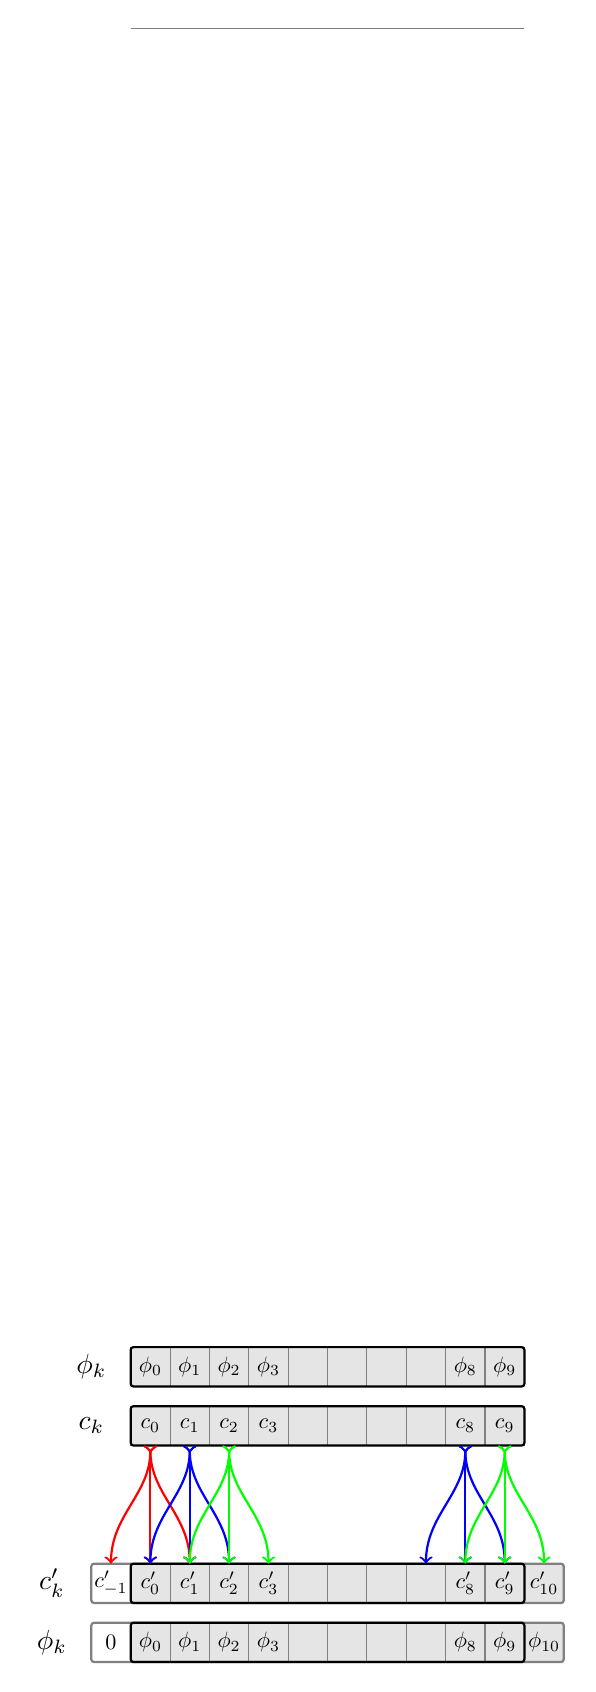
\begin{tikzpicture}
  \coordinate (co0) at (0.25, 2.0);
  \coordinate (co1) at (0.75, 2.0);
  \coordinate (co2) at (1.25, 2.0);
  \coordinate (co3) at (1.75, 2.0);
  \coordinate (co8) at (4.25, 2.0);
  \coordinate (co9) at (4.75, 2.0);

  \coordinate (cpm1) at (-0.25, 0.5);
  \coordinate (cp0) at (0.25, 0.5);
  \coordinate (cp1) at (0.75, 0.5);
  \coordinate (cp2) at (1.25, 0.5);
  \coordinate (cp3) at (1.75, 0.5);
  \coordinate (cp7) at (3.75, 0.5);
  \coordinate (cp8) at (4.25, 0.5);
  \coordinate (cp9) at (4.75, 0.5);
  \coordinate (cp10) at (5.25, 0.5);

  % upper
  \fill[gray!20, rounded corners=1] (0.0,2.0) rectangle (5.0,2.5);
  \draw[step=5mm, gray] (0,2.0) grid (5,2.5);
  \draw[black, thick, rounded corners=1] (0.0,2.0) rectangle (5.0,2.5);

  \fill[gray!20, rounded corners=1] (0.0,2.75) rectangle (5.0,3.25);
  \draw[step=5mm, ystep=20cm, gray] (0.0,2.75) grid (5.0,3.25);
  \draw[black, thick, rounded corners=1] (0.0,2.75) rectangle (5.0,3.25);

  % lower
  \fill[gray!20, rounded corners=1] (0.0,-0.75) rectangle (5.5,-0.25);
  \draw[step=5mm, ystep=20cm, gray] (0.0,-0.75) grid (5.0,-0.25);
  \draw[gray, thick, rounded corners=1] (-0.5,-0.75) rectangle (5.5,-0.25);
  \draw[black, thick, rounded corners=1] (0.0,-0.75) rectangle (5.0,-0.25);

  \fill[gray!20, rounded corners=1] (0.0,0.0) rectangle (5.5,0.5);
  \draw[step=5mm, gray] (0.0,0.0) grid (5.0,0.5);
  \draw[gray, thick, rounded corners=1] (-0.5,0.0) rectangle (5.5,0.5);
  \draw[black, thick, rounded corners=1] (0.0,0.0) rectangle (5.0,0.5);

  \draw[>->, thick, color=red] (co0) to[out=270,in=90] (cpm1);
  \draw[>->, thick, color=red] (co0) to[out=270,in=90] (cp0);
  \draw[>->, thick, color=red] (co0) to[out=270,in=90] (cp1);

  \draw[>->, thick, color=blue] (co1) to[out=270,in=90] (cp0);
  \draw[>->, thick, color=blue] (co1) to[out=270,in=90] (cp1);
  \draw[>->, thick, color=blue] (co1) to[out=270,in=90] (cp2);

  \draw[>->, thick, color=green] (co2) to[out=270,in=90] (cp1);
  \draw[>->, thick, color=green] (co2) to[out=270,in=90] (cp2);
  \draw[>->, thick, color=green] (co2) to[out=270,in=90] (cp3);

  \draw[>->, thick, color=blue] (co8) to[out=270,in=90] (cp7);
  \draw[>->, thick, color=blue] (co8) to[out=270,in=90] (cp8);
  \draw[>->, thick, color=blue] (co8) to[out=270,in=90] (cp9);

  \draw[>->, thick, color=green] (co9) to[out=270,in=90] (cp8);
  \draw[>->, thick, color=green] (co9) to[out=270,in=90] (cp9);
  \draw[>->, thick, color=green] (co9) to[out=270,in=90] (cp10);

  \node[scale=0.8] at (0.25,2.25) [black] {$c_0$};
  \node[scale=0.8] at (0.75,2.25) [black] {$c_1$};
  \node[scale=0.8] at (1.25,2.25) [black] {$c_2$};
  \node[scale=0.8] at (1.75,2.25) [black] {$c_3$};
  \node[scale=0.8] at (4.25,2.25) [black] {$c_8$};
  \node[scale=0.8] at (4.75,2.25) [black] {$c_9$};

  \node[scale=0.8] at (-0.25,0.25) [black] {$c^\prime_{-1}$};
  \node[scale=0.8] at (0.25,0.25) [black] {$c^\prime_0$};
  \node[scale=0.8] at (0.75,0.25) [black] {$c^\prime_1$};
  \node[scale=0.8] at (1.25,0.25) [black] {$c^\prime_2$};
  \node[scale=0.8] at (1.75,0.25) [black] {$c^\prime_3$};
  \node[scale=0.8] at (4.25,0.25) [black] {$c^\prime_8$};
  \node[scale=0.8] at (4.75,0.25) [black] {$c^\prime_9$};
  \node[scale=0.8] at (5.25,0.25) [black] {$c^\prime_{10}$};

  \node[scale=0.8] at (0.25,3.0) [black] {$\phi_0$};
  \node[scale=0.8] at (0.75,3.0) [black] {$\phi_1$};
  \node[scale=0.8] at (1.25,3.0) [black] {$\phi_2$};
  \node[scale=0.8] at (1.75,3.0) [black] {$\phi_3$};
  \node[scale=0.8] at (4.25,3.0) [black] {$\phi_8$};
  \node[scale=0.8] at (4.75,3.0) [black] {$\phi_9$};

  \node[scale=0.8] at (-0.25,-0.5) [black] {$0$};
  \node[scale=0.8] at (0.25,-0.5) [black] {$\phi_0$};
  \node[scale=0.8] at (0.75,-0.5) [black] {$\phi_1$};
  \node[scale=0.8] at (1.25,-0.5) [black] {$\phi_2$};
  \node[scale=0.8] at (1.75,-0.5) [black] {$\phi_3$};
  \node[scale=0.8] at (4.25,-0.5) [black] {$\phi_8$};
  \node[scale=0.8] at (4.75,-0.5) [black] {$\phi_9$};
  \node[scale=0.8] at (5.25,-0.5) [black] {$\phi_{10}$};

  \node at (-0.5,3.0) [black] {$\phi_{k}$};
  \node at (-1.0,-0.5) [black] {$\phi_{k}$};
  \node at (-0.5,2.25) [black] {$c_{k}$};
  \node at (-1.0,0.25) [black] {$c^\prime_{k}$};
\end{tikzpicture}

  \caption[Scatter-type stencil in 1D] {The scatter-type stencil application for
           computing the gradient $y\Phi$. The upper two arrays show the initial linear
           combination $\Phi$ consisting of basis functions $\phi_k$ and coefficients $c_k$.
           The lower two arrays show the linear combination of $\diff{\Phi}{x}$ consisting
           of the same basis functions $\phi_k$ and new coefficients $c_k^\prime$.
           Each of the triple arrows represents the computation for a fixed $\vec{k} \in \mathfrak{K}$
           (formula \eqref{eq:grad_basis_function_DD}), not all computations are shown.
           We see that the basis shape $\overline{\mathfrak{K}}$ for the gradient
           has to be larger. And also that we write to several elements not part
           of the original basis shape $\mathfrak{K}$. We drop the coefficient
           $c_{-1}^\prime$ (because $\phi_{-1} \equiv 0$).
           The original basis shape $\mathfrak{K}$ is represented by the black rectangle
           and the actual basis shapes are shown shaded grey.}
  \label{fig:grad_phi_kl_scatter_stencil_1D}
\end{figure}

\begin{figure}
  \centering
  \begin{tikzpicture}[scale=1,every node/.style={minimum size=0.5cm},on grid]

  \begin{scope}[
      yshift=-100,
      every node/.append style={yslant=0.5, xslant=-1.3},
      yslant=0.5,
      xslant=-1.3
    ]
    \coordinate (c32) at (1.75, 1.25);
    \coordinate (co25) at (1.25, 2.75);
  \end{scope}

  \begin{scope}[
      yshift=-160,
      every node/.append style={yslant=0.5, xslant=-1.3},
      yslant=0.5,
      xslant=-1.3
    ]
    \coordinate (cp42) at (2.25, 1.25);
    \coordinate (cp32) at (1.75, 1.25);
    \coordinate (cp22) at (1.25, 1.25);
    \coordinate (cp33) at (1.75, 1.75);
    \coordinate (cp31) at (1.75, 0.75);

    \coordinate (cop15) at (0.75, 2.75);
    \coordinate (cop25) at (1.25, 2.75);
    \coordinate (cop35) at (1.75, 2.75);
    \coordinate (cop24) at (1.25, 2.25);
    \coordinate (cop26) at (1.25, 3.25);
  \end{scope}

  % lower plane
  \begin{scope}[
      yshift=-160,
      every node/.append style={yslant=0.5, xslant=-1.3},
      yslant=0.5,
      xslant=-1.3
    ]
    \draw[step=5mm, thin, gray] (-0.5,-0.5) grid (3.5,3.5);

    \fill[blue!60] (2,1) rectangle (2.5,1.5);
    \node at (cp42) [draw, color=blue] {};%{$c^\prime_{4,2}$};

    \fill[blue!60] (1.5,1) rectangle (2.0,1.5);
    \node at (cp32) [draw, color=blue] {};%{$c^\prime_{3,2}$};

    \fill[blue!60] (1,1) rectangle (1.5,1.5);
    \node at (cp22) [draw, color=blue] {};%{$c^\prime_{2,2}$};

    \fill[blue!60] (1.5,1.5) rectangle (2.0,2.0);
    \node at (cp33) [draw, color=blue] {};%{$c^\prime_{3,3}$};

    \fill[blue!60] (1.5,0.5) rectangle (2.0,1.0);
    \node at (cp31) [draw, color=blue] {};%{$c^\prime_{3,1}$};

    \fill[orange!60] (0.5,2.5) rectangle (1.0,3.0);
    \node at (cop15) [draw, color=orange] {};%{$c^\prime_{1,5}$};

    \fill[orange!60] (1.0,2.5) rectangle (1.5,3.0);
    \node at (cop25) [draw, color=orange] {};%{$c^\prime_{2,5}$};

    \fill[orange!60] (1.5,2.5) rectangle (2.0,3.0);
    \node at (cop35) [draw, color=orange] {};%{$c^\prime_{3,5}$};

    \fill[orange!60] (1.0,2.0) rectangle (1.5,2.5);
    \node at (cop24) [draw, color=orange] {};%{$c^\prime_{2,4}$};

    \fill[orange!60] (1.0,3.0) rectangle (1.5,3.5);
    \node at (cop26) [draw, color=orange] {};%{$c^\prime_{2,6}$};

    \draw[black,thick, rounded corners=1] (0,0) rectangle (3,3);
    \draw[gray,thick, rounded corners=1] (-0.5,-0.5) rectangle (3.5,3.5);
  \end{scope}

  % arrows
  \begin{scope}
    \draw[>->, thick] (c32) node[left,scale=1.3] {} to[out=270,in=90] (cp42);
    \draw[>->, thick] (c32) node[left,scale=1.3] {} to[out=270,in=90] (cp32);
    \draw[>->, thick] (c32) node[left,scale=1.3] {} to[out=270,in=90] (cp22);
    \draw[>->, thick] (c32) node[left,scale=1.3] {} to[out=270,in=90] (cp33);
    \draw[>->, thick] (c32) node[left,scale=1.3] {} to[out=270,in=90] (cp31);

    \draw[>->, thick] (co25) node[left,scale=1.3] {} to[out=270,in=90] (cop24);
    \draw[>->, thick] (co25) node[left,scale=1.3] {} to[out=270,in=90] (cop25);
    \draw[>->, thick] (co25) node[left,scale=1.3] {} to[out=270,in=90] (cop26);
    \draw[>->, thick] (co25) node[left,scale=1.3] {} to[out=270,in=90] (cop15);
    \draw[>->, thick] (co25) node[left,scale=1.3] {} to[out=270,in=90] (cop35);
  \end{scope}

  % upper plane
  \begin{scope}[
      yshift=-100,
      every node/.append style={yslant=0.5, xslant=-1.3},
      yslant=0.5,
      xslant=-1.3
    ]
    \fill[white,fill opacity=0.8] (0,0) rectangle (3,3);
    \draw[step=5mm, thin, gray] (0,0) grid (3,3);

    \fill[blue!60] (1.5,1) rectangle (2.0,1.5);
    \node at (c32) [draw, color=blue] {};%{$c_{3,2}$};

    \fill[orange!60] (1.0,2.5) rectangle (1.5,3.0);
    \node at (co25) [draw, color=orange] {};%{$c_{2,5}$};

    \draw[black,thick, rounded corners=1] (0,0) rectangle (3,3);
  \end{scope}

  \node at (-3.25cm,-1.5cm) [black] {$c_{k,l}$};
  \node at (-4cm,-5.5cm) [black] {$\vec{c}^\prime_{k,l}$};
\end{tikzpicture}

  \caption[Scatter-type stencil in 2D] {The scatter-type stencil application for
           computing the gradient $y\Phi$. The upper array (plane) shows the
           coefficients $c_{\vec{k}}$ of the initial linear combination $\Phi(\vec{x})$.
           The lower array (plane) shows the coefficients $\vec{c}^\prime_{\vec{k}}$ of the
           linear combination of $\nabla\Phi(\vec{x})$ where each square is not a single
           number but stands for a whole vector. Each arrow bundle represents the
           computation for a fixed $\vec{k} \in \mathfrak{K}$ (formula
           \eqref{eq:grad_basis_function_DD}), not all computations are shown.
           The original basis shape $\mathfrak{K}$ is given by the black rectangle.
           We then see that the basis shape $\overline{\mathfrak{K}}$ for the gradient
           is larger by one square on each side. (But we again drop all coefficients
           with negative index.)
           The orange stencil shows that we sometimes have to write to elements
           (coefficients) that are not part of the original basis shape. Therefore
           we need to extend the basis shape where the whole lower plane stands
           for $\overline{\mathfrak{K}}$.
}
  \label{fig:grad_phi_kl_scatter_stencil_2D}
\end{figure}

\begin{algorithm}
\caption{Compute the gradient $y \Phi$ by scatter-type stencil application}
\label{al:grad_phi_scatter_type}
\begin{algorithmic}
  \REQUIRE Scalar wavepacket $\Phi$ in $D$ space dimensions
  \REQUIRE Basis shape $\mathfrak{K}$ (including linearisation mapping $\mu_{\mathfrak{K}}$) of $\Phi$
  \REQUIRE Parameters $\Pi$ and coefficients $\{c_{\vec{k}}\}$ of $\Phi$

  \STATE // Extend the basis shape $\mathfrak{K}$
  \STATE $\overline{\mathfrak{K}} \assign \text{\bf{extend\_basis\_shape}}(\mathfrak{K})$

  \STATE // Storage space for the result
  \STATE $\mat{c}^\prime = \mat{0} \in \mathbb{C}^{D \times |\overline{\mathfrak{K}}|}$

  \STATE // Iterate over original basis shape
  \FOR{$\vec{k} \in \mathfrak{K}$}

    \STATE // Central node
    \STATE $\mat{c}^\prime[:,\mu_{\overline{\mathfrak{K}}}(\vec{k})] =
            \mat{c}^\prime[:,\mu_{\overline{\mathfrak{K}}}(\vec{k})] +
            c_{\vec{k}} \, \vec{p}$

    \STATE // Backward neighbours
    \FOR{$d = 0$ \TO $d = D-1$}
      \STATE $\vec{k}^\prime = \vec{k} - \vec{e}^d$
      \IF{$\vec{k}^\prime \in \overline{\mathfrak{K}}$}
        \STATE $\mat{c}^\prime[:,\mu_{\overline{\mathfrak{K}}}(\vec{k}^\prime)] =
                \mat{c}^\prime[:,\mu_{\overline{\mathfrak{K}}}(\vec{k}^\prime)] +
                \sqrt{\frac{\varepsilon^2}{2}} \sqrt{\vec{k}[d]} \, c_{\vec{k}} \, \conj{\mat{P}}[:,d]$
      \ENDIF
    \ENDFOR

    \STATE // Forward neighbours
    \FOR{$d = 0$ \TO $d = D-1$}
      \STATE $\vec{k}^\prime = \vec{k} + \vec{e}^d$
      \IF{$\vec{k}^\prime \in \overline{\mathfrak{K}}$}
        \STATE $\mat{c}^\prime[:,\mu_{\overline{\mathfrak{K}}}(\vec{k}^\prime)] =
                \mat{c}^\prime[:,\mu_{\overline{\mathfrak{K}}}(\vec{k}^\prime)] +
                \sqrt{\frac{\varepsilon^2}{2}} \sqrt{\vec{k}[d]+1} \, c_{\vec{k}} \, \mat{P}[:,d]$
      \ENDIF
    \ENDFOR

  \ENDFOR
  \RETURN $\overline{\mathfrak{K}}$ and $\mat{c}^\prime$
\end{algorithmic}
\end{algorithm}


\subsection{An example}


As an example we take a wavepacket $\Ket{\Psi}$ in two space dimensions with the
following parameter set $\Pi = \{\vec{0}, \vec{0}, \id, i \id \}$ and $\varepsilon = 0.6$.
The coefficients are set to the values printed in the next table.

\begin{center}
\begin{tabular}{l r}
$\vec{k}$ & $c_{\vec{k}}$ \\
\hline
$(0,0)$ & $0.5$ \\
$(0,1)$ & $0.5$ \\
$(1,1)$ & $0.5$ \\
$(2,1)$ & $0.5$
\end{tabular}
\end{center}

A plot of the wavepacket evaluated on a small region of position space is shown
in figure \ref{fig:wavepacket_original}.

\begin{figure}
  \centering
  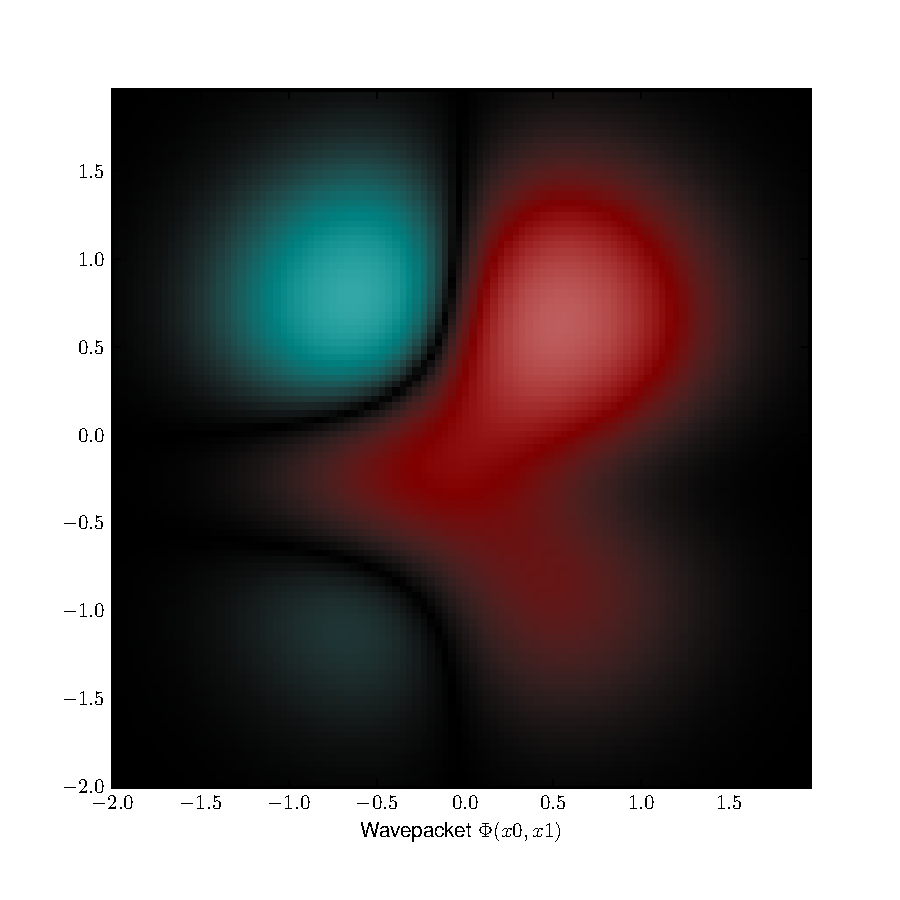
\includegraphics[scale=0.3]{./fig/wavepacket_original.pdf}
  \caption[Wavepacket of the gradient example]{The wavepacket $\Ket{\Psi}$.}
  \label{fig:wavepacket_original}
\end{figure}

Next we compute the gradient $-i \varepsilon \nabla \Psi$ by one of the above
methods. For the new coefficients $\vec{c}_{\vec{k}}$ we get the values (only
non-zero ones) shown in the next table. The two components of the gradient
are plotted in figure \ref{fig:wavepacket_gradient}.

\begin{center}
\begin{tabular}{l r r}
$\vec{k}$ & $x_0$ component of $\vec{c}_{\vec{k}}$ &  $x_1$ component of $\vec{c}_{\vec{k}}$ \\
\hline
$(0,0)$ &$0$                            & $- 0.21213203 \mathbf{\imath}$ \\
$(0,1)$ &$- 0.21213203 \mathbf{\imath}$ & $0.21213203 \mathbf{\imath}$ \\
$(1,0)$ &$0.21213203 \mathbf{\imath}$   & $- 0.21213203 \mathbf{\imath}$ \\
$(1,1)$ &$- 0.08786797 \mathbf{\imath}$ & $0$  \\
$(2,0)$ &$0$                            & $- 0.21213203 \mathbf{\imath}$ \\
$(2,1)$ &$0.3 \mathbf{\imath}$          & $0$  \\
$(3,1)$ &$0.36742346 \mathbf{\imath}$   & $0$  \\
$(0,2)$ &$0$                            & $0.3 \mathbf{\imath}$ \\
$(1,2)$ &$0$                            & $0.3 \mathbf{\imath}$ \\
$(2,2)$ &$0$                            & $0.3 \mathbf{\imath}$ \\
\end{tabular}

\end{center}\begin{figure}
  \centering
  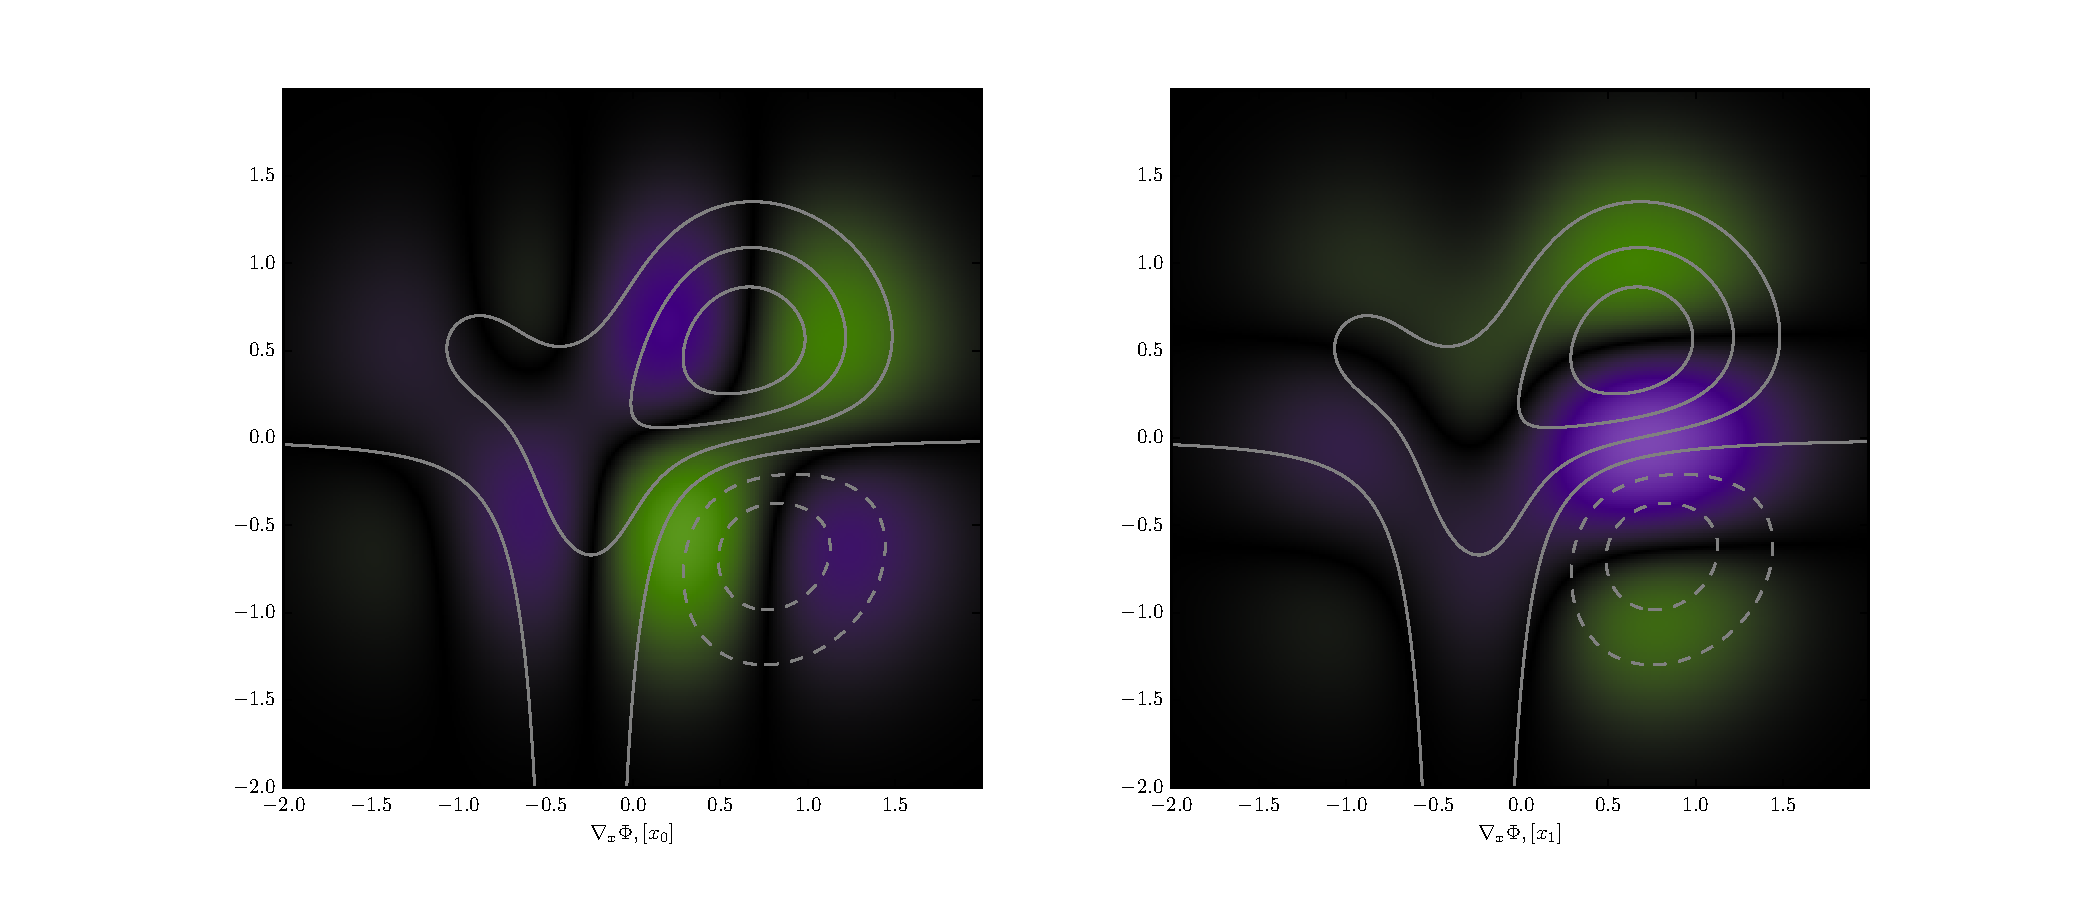
\includegraphics[scale=0.32]{./fig/wavepacket_gradient.pdf}
  \caption[Plots of the gradient example]
          {The $x_0$ (left) and $x_1$ (right) components of the gradient
           $-i \varepsilon \nabla \Psi$. The wavepacket $\Psi$ is indicated
           by some contour levels just for reference.}
  \label{fig:wavepacket_gradient}
\end{figure}

Finally, figure \ref{fig:wavepacket_coefficients} shows again the coefficients
of both, the original wavepacket and the two components of its gradient.

\begin{figure}
  \centering
  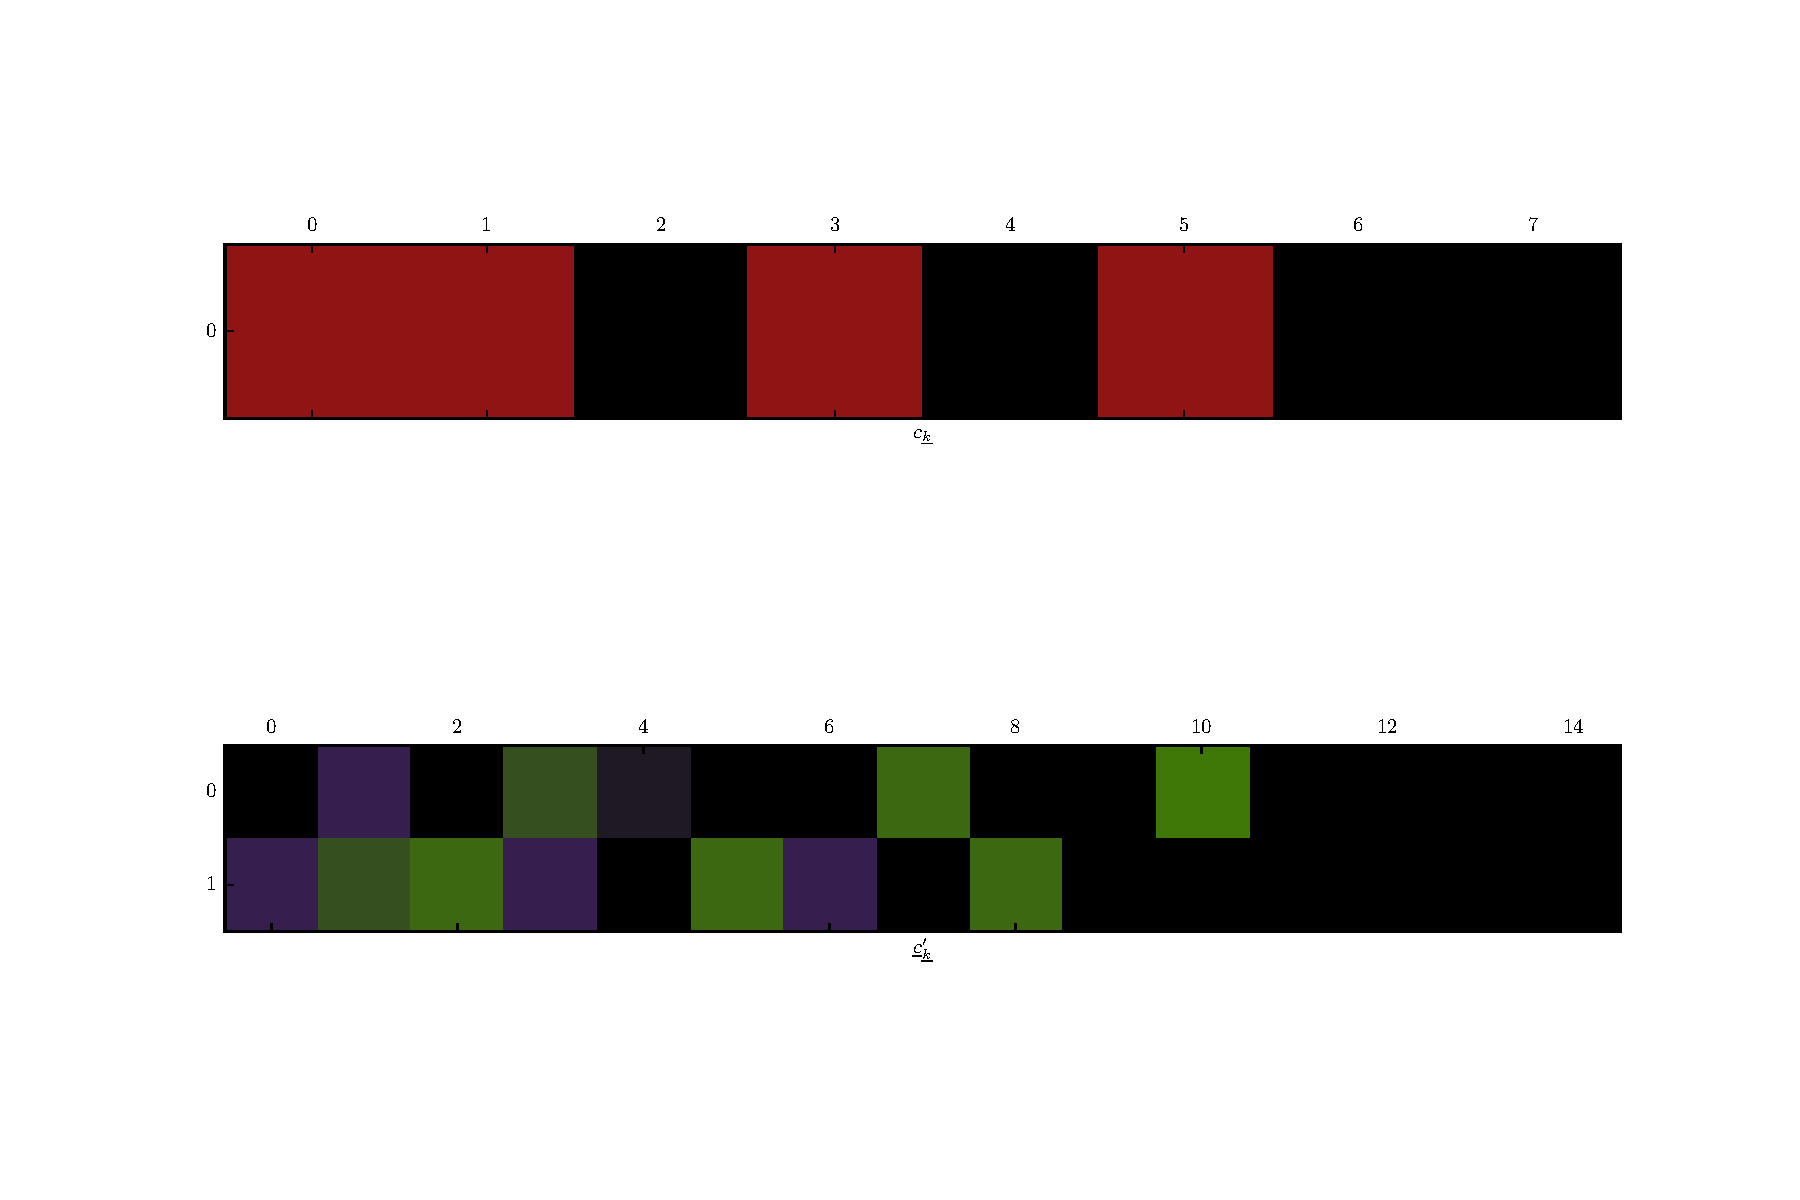
\includegraphics[scale=0.6]{./fig/wavepacket_coefficients.pdf}
  \caption[Coefficients of the gradient example]
         {Coefficients $c_{\vec{k}}$ of $\Psi$ (left) and $\vec{c}_{\vec{k}}$ of
          $-i \varepsilon \nabla \Psi$ (right). Notice also the different basis
          sizes $|\mathfrak{K}|$ of 8 and 15.}
  \label{fig:wavepacket_coefficients}
\end{figure}
